\documentclass[twoside]{book}

% Packages required by doxygen
\usepackage{fixltx2e}
\usepackage{calc}
\usepackage{doxygen}
\usepackage{graphicx}
\usepackage[utf8]{inputenc}
\usepackage{makeidx}
\usepackage{multicol}
\usepackage{multirow}
\PassOptionsToPackage{warn}{textcomp}
\usepackage{textcomp}
\usepackage[nointegrals]{wasysym}
\usepackage[table]{xcolor}

% Font selection
\usepackage[T1]{fontenc}
\usepackage{mathptmx}
\usepackage[scaled=.90]{helvet}
\usepackage{courier}
\usepackage{amssymb}
\usepackage{sectsty}
\renewcommand{\familydefault}{\sfdefault}
\allsectionsfont{%
  \fontseries{bc}\selectfont%
  \color{darkgray}%
}
\renewcommand{\DoxyLabelFont}{%
  \fontseries{bc}\selectfont%
  \color{darkgray}%
}
\newcommand{\+}{\discretionary{\mbox{\scriptsize$\hookleftarrow$}}{}{}}

% Page & text layout
\usepackage{geometry}
\geometry{%
  a4paper,%
  top=2.5cm,%
  bottom=2.5cm,%
  left=2.5cm,%
  right=2.5cm%
}
\tolerance=750
\hfuzz=15pt
\hbadness=750
\setlength{\emergencystretch}{15pt}
\setlength{\parindent}{0cm}
\setlength{\parskip}{0.2cm}
\makeatletter
\renewcommand{\paragraph}{%
  \@startsection{paragraph}{4}{0ex}{-1.0ex}{1.0ex}{%
    \normalfont\normalsize\bfseries\SS@parafont%
  }%
}
\renewcommand{\subparagraph}{%
  \@startsection{subparagraph}{5}{0ex}{-1.0ex}{1.0ex}{%
    \normalfont\normalsize\bfseries\SS@subparafont%
  }%
}
\makeatother

% Headers & footers
\usepackage{fancyhdr}
\pagestyle{fancyplain}
\fancyhead[LE]{\fancyplain{}{\bfseries\thepage}}
\fancyhead[CE]{\fancyplain{}{}}
\fancyhead[RE]{\fancyplain{}{\bfseries\leftmark}}
\fancyhead[LO]{\fancyplain{}{\bfseries\rightmark}}
\fancyhead[CO]{\fancyplain{}{}}
\fancyhead[RO]{\fancyplain{}{\bfseries\thepage}}
\fancyfoot[LE]{\fancyplain{}{}}
\fancyfoot[CE]{\fancyplain{}{}}
\fancyfoot[RE]{\fancyplain{}{\bfseries\scriptsize Generated on Fri Jan 15 2016 21\+:26\+:47 for Open\+Securiy\+S\+M\+S by Doxygen }}
\fancyfoot[LO]{\fancyplain{}{\bfseries\scriptsize Generated on Fri Jan 15 2016 21\+:26\+:47 for Open\+Securiy\+S\+M\+S by Doxygen }}
\fancyfoot[CO]{\fancyplain{}{}}
\fancyfoot[RO]{\fancyplain{}{}}
\renewcommand{\footrulewidth}{0.4pt}
\renewcommand{\chaptermark}[1]{%
  \markboth{#1}{}%
}
\renewcommand{\sectionmark}[1]{%
  \markright{\thesection\ #1}%
}

% Indices & bibliography
\usepackage{natbib}
\usepackage[titles]{tocloft}
\setcounter{tocdepth}{3}
\setcounter{secnumdepth}{5}
\makeindex

% Hyperlinks (required, but should be loaded last)
\usepackage{ifpdf}
\ifpdf
  \usepackage[pdftex,pagebackref=true]{hyperref}
\else
  \usepackage[ps2pdf,pagebackref=true]{hyperref}
\fi
\hypersetup{%
  colorlinks=true,%
  linkcolor=blue,%
  citecolor=blue,%
  unicode%
}

% Custom commands
\newcommand{\clearemptydoublepage}{%
  \newpage{\pagestyle{empty}\cleardoublepage}%
}


%===== C O N T E N T S =====

\begin{document}

% Titlepage & ToC
\hypersetup{pageanchor=false,
             bookmarks=true,
             bookmarksnumbered=true,
             pdfencoding=unicode
            }
\pagenumbering{roman}
\begin{titlepage}
\vspace*{7cm}
\begin{center}%
{\Large Open\+Securiy\+S\+M\+S }\\
\vspace*{1cm}
{\large Generated by Doxygen 1.8.7}\\
\vspace*{0.5cm}
{\small Fri Jan 15 2016 21:26:47}\\
\end{center}
\end{titlepage}
\clearemptydoublepage
\tableofcontents
\clearemptydoublepage
\pagenumbering{arabic}
\hypersetup{pageanchor=true}

%--- Begin generated contents ---
\chapter{Namespace Index}
\section{Packages}
Here are the packages with brief descriptions (if available)\+:\begin{DoxyCompactList}
\item\contentsline{section}{\hyperlink{a00031}{org} }{\pageref{a00031}}{}
\item\contentsline{section}{\hyperlink{a00032}{org.\+opensecurity} }{\pageref{a00032}}{}
\item\contentsline{section}{\hyperlink{a00033}{org.\+opensecurity.\+sms} }{\pageref{a00033}}{}
\item\contentsline{section}{\hyperlink{a00034}{org.\+opensecurity.\+sms.\+controller} }{\pageref{a00034}}{}
\item\contentsline{section}{\hyperlink{a00035}{org.\+opensecurity.\+sms.\+model} }{\pageref{a00035}}{}
\item\contentsline{section}{\hyperlink{a00036}{org.\+opensecurity.\+sms.\+model.\+model\+View} }{\pageref{a00036}}{}
\item\contentsline{section}{\hyperlink{a00037}{org.\+opensecurity.\+sms.\+model.\+model\+View.\+conversation} }{\pageref{a00037}}{}
\item\contentsline{section}{\hyperlink{a00038}{org.\+opensecurity.\+sms.\+model.\+model\+View.\+list\+Conversation} }{\pageref{a00038}}{}
\item\contentsline{section}{\hyperlink{a00039}{org.\+opensecurity.\+sms.\+model.\+security} }{\pageref{a00039}}{}
\item\contentsline{section}{\hyperlink{a00040}{org.\+opensecurity.\+sms.\+view} }{\pageref{a00040}}{}
\end{DoxyCompactList}

\chapter{Hierarchical Index}
\section{Class Hierarchy}
This inheritance list is sorted roughly, but not completely, alphabetically\+:\begin{DoxyCompactList}
\item \contentsline{section}{A\+E\+S}{\pageref{a00001}}{}
\item \contentsline{section}{Conversation\+Item}{\pageref{a00007}}{}
\begin{DoxyCompactList}
\item \contentsline{section}{Bubble}{\pageref{a00004}}{}
\end{DoxyCompactList}
\item \contentsline{section}{D\+A\+O}{\pageref{a00009}}{}
\item On\+Gesture\+Listener\begin{DoxyCompactList}
\item \contentsline{section}{Popup\+Conversation\+Activity}{\pageref{a00013}}{}
\end{DoxyCompactList}
\item \contentsline{section}{R\+S\+A}{\pageref{a00014}}{}
\item \contentsline{section}{Serializer}{\pageref{a00015}}{}
\item Activity\begin{DoxyCompactList}
\item \contentsline{section}{Popup\+Conversation\+Activity}{\pageref{a00013}}{}
\end{DoxyCompactList}
\item App\+Compat\+Activity\begin{DoxyCompactList}
\item \contentsline{section}{Conversation\+Activity}{\pageref{a00006}}{}
\item \contentsline{section}{Open\+Security\+S\+M\+S}{\pageref{a00011}}{}
\end{DoxyCompactList}
\item Array\+Adapter\begin{DoxyCompactList}
\item \contentsline{section}{Array\+Bubble\+Adapter}{\pageref{a00002}}{}
\item \contentsline{section}{Array\+Convers\+Adapter}{\pageref{a00003}}{}
\end{DoxyCompactList}
\item Broadcast\+Receiver\begin{DoxyCompactList}
\item \contentsline{section}{S\+M\+S\+Receiver}{\pageref{a00016}}{}
\end{DoxyCompactList}
\item Serializable\begin{DoxyCompactList}
\item \contentsline{section}{Contact}{\pageref{a00005}}{}
\item \contentsline{section}{Conversation\+Line}{\pageref{a00008}}{}
\end{DoxyCompactList}
\item S\+Q\+Lite\+Open\+Helper\begin{DoxyCompactList}
\item \contentsline{section}{Database\+Handler}{\pageref{a00010}}{}
\item \contentsline{section}{Password\+Db\+Helper}{\pageref{a00012}}{}
\end{DoxyCompactList}
\end{DoxyCompactList}

\chapter{Class Index}
\section{Class List}
Here are the classes, structs, unions and interfaces with brief descriptions\+:\begin{DoxyCompactList}
\item\contentsline{section}{\hyperlink{a00001}{A\+E\+S} }{\pageref{a00001}}{}
\item\contentsline{section}{\hyperlink{a00002}{Array\+Bubble\+Adapter} }{\pageref{a00002}}{}
\item\contentsline{section}{\hyperlink{a00003}{Array\+Convers\+Adapter} }{\pageref{a00003}}{}
\item\contentsline{section}{\hyperlink{a00004}{Bubble} }{\pageref{a00004}}{}
\item\contentsline{section}{\hyperlink{a00005}{Contact} }{\pageref{a00005}}{}
\item\contentsline{section}{\hyperlink{a00006}{Controller} }{\pageref{a00006}}{}
\item\contentsline{section}{\hyperlink{a00007}{Conversation\+Activity} }{\pageref{a00007}}{}
\item\contentsline{section}{\hyperlink{a00008}{Conversation\+Item} }{\pageref{a00008}}{}
\item\contentsline{section}{\hyperlink{a00009}{Conversation\+Line} }{\pageref{a00009}}{}
\item\contentsline{section}{\hyperlink{a00010}{Open\+Security\+S\+M\+S} }{\pageref{a00010}}{}
\item\contentsline{section}{\hyperlink{a00011}{Password\+Db\+Helper} }{\pageref{a00011}}{}
\item\contentsline{section}{\hyperlink{a00012}{Popup\+Conversation\+Activity} }{\pageref{a00012}}{}
\item\contentsline{section}{\hyperlink{a00013}{R\+S\+A} }{\pageref{a00013}}{}
\item\contentsline{section}{\hyperlink{a00014}{Serializer} }{\pageref{a00014}}{}
\item\contentsline{section}{\hyperlink{a00015}{S\+M\+S\+Receiver} }{\pageref{a00015}}{}
\end{DoxyCompactList}

\chapter{File Index}
\section{File List}
Here is a list of all files with brief descriptions\+:\begin{DoxyCompactList}
\item\contentsline{section}{app/src/main/java/org/opensecurity/sms/model/\hyperlink{a00017}{Contact.\+java} }{\pageref{a00017}}{}
\item\contentsline{section}{app/src/main/java/org/opensecurity/sms/model/\hyperlink{a00018}{D\+A\+O.\+java} }{\pageref{a00018}}{}
\item\contentsline{section}{app/src/main/java/org/opensecurity/sms/model/\hyperlink{a00019}{Database\+Handler.\+java} }{\pageref{a00019}}{}
\item\contentsline{section}{app/src/main/java/org/opensecurity/sms/model/\hyperlink{a00028}{Serializer.\+java} }{\pageref{a00028}}{}
\item\contentsline{section}{app/src/main/java/org/opensecurity/sms/model/\hyperlink{a00029}{S\+M\+S\+Receiver.\+java} }{\pageref{a00029}}{}
\item\contentsline{section}{app/src/main/java/org/opensecurity/sms/model/model\+View/conversation/\hyperlink{a00020}{Array\+Bubble\+Adapter.\+java} }{\pageref{a00020}}{}
\item\contentsline{section}{app/src/main/java/org/opensecurity/sms/model/model\+View/conversation/\hyperlink{a00021}{Bubble.\+java} }{\pageref{a00021}}{}
\item\contentsline{section}{app/src/main/java/org/opensecurity/sms/model/model\+View/conversation/\hyperlink{a00022}{Conversation\+Item.\+java} }{\pageref{a00022}}{}
\item\contentsline{section}{app/src/main/java/org/opensecurity/sms/model/model\+View/list\+Conversation/\hyperlink{a00023}{Array\+Convers\+Adapter.\+java} }{\pageref{a00023}}{}
\item\contentsline{section}{app/src/main/java/org/opensecurity/sms/model/model\+View/list\+Conversation/\hyperlink{a00024}{Conversation\+Line.\+java} }{\pageref{a00024}}{}
\item\contentsline{section}{app/src/main/java/org/opensecurity/sms/model/security/\hyperlink{a00025}{A\+E\+S.\+java} }{\pageref{a00025}}{}
\item\contentsline{section}{app/src/main/java/org/opensecurity/sms/model/security/\hyperlink{a00026}{Password\+Db\+Helper.\+java} }{\pageref{a00026}}{}
\item\contentsline{section}{app/src/main/java/org/opensecurity/sms/model/security/\hyperlink{a00027}{R\+S\+A.\+java} }{\pageref{a00027}}{}
\item\contentsline{section}{app/src/main/java/org/opensecurity/sms/view/\hyperlink{a00030}{Conversation\+Activity.\+java} }{\pageref{a00030}}{}
\item\contentsline{section}{app/src/main/java/org/opensecurity/sms/view/\hyperlink{a00031}{Open\+Security\+S\+M\+S.\+java} }{\pageref{a00031}}{}
\item\contentsline{section}{app/src/main/java/org/opensecurity/sms/view/\hyperlink{a00032}{Popup\+Conversation\+Activity.\+java} }{\pageref{a00032}}{}
\end{DoxyCompactList}

\chapter{Namespace Documentation}
\hypertarget{a00033}{\section{Package org.\+opensecurity.\+sms}
\label{a00033}\index{org.\+opensecurity.\+sms@{org.\+opensecurity.\+sms}}
}
\subsection*{Packages}
\begin{DoxyCompactItemize}
\item 
package \hyperlink{a00034}{controller}
\item 
package \hyperlink{a00035}{model}
\item 
package \hyperlink{a00040}{view}
\end{DoxyCompactItemize}

\hypertarget{a00034}{\section{Package org.\+opensecurity.\+sms.\+controller}
\label{a00034}\index{org.\+opensecurity.\+sms.\+controller@{org.\+opensecurity.\+sms.\+controller}}
}
\subsection*{Classes}
\begin{DoxyCompactItemize}
\item 
class \hyperlink{a00006}{Controller}
\end{DoxyCompactItemize}

\hypertarget{a00035}{\section{Package org.\+opensecurity.\+sms.\+model}
\label{a00035}\index{org.\+opensecurity.\+sms.\+model@{org.\+opensecurity.\+sms.\+model}}
}
\subsection*{Packages}
\begin{DoxyCompactItemize}
\item 
package \hyperlink{a00036}{model\+View}
\item 
package \hyperlink{a00039}{security}
\end{DoxyCompactItemize}
\subsection*{Classes}
\begin{DoxyCompactItemize}
\item 
class \hyperlink{a00005}{Contact}
\item 
class \hyperlink{a00014}{Serializer}
\item 
class \hyperlink{a00015}{S\+M\+S\+Receiver}
\end{DoxyCompactItemize}

\hypertarget{a00036}{\section{Package org.\+opensecurity.\+sms.\+model}
\label{a00036}\index{org.\+opensecurity.\+sms.\+model@{org.\+opensecurity.\+sms.\+model}}
}
\subsection*{Packages}
\begin{DoxyCompactItemize}
\item 
package \hyperlink{a00037}{model\+View}
\item 
package \hyperlink{a00040}{security}
\end{DoxyCompactItemize}
\subsection*{Classes}
\begin{DoxyCompactItemize}
\item 
class \hyperlink{a00005}{Contact}
\item 
class \hyperlink{a00009}{D\+A\+O}
\item 
class \hyperlink{a00010}{Database\+Handler}
\item 
class \hyperlink{a00015}{Serializer}
\item 
class \hyperlink{a00016}{S\+M\+S\+Receiver}
\end{DoxyCompactItemize}

\hypertarget{a00037}{\section{Package org.\+opensecurity.\+sms.\+model.\+model\+View}
\label{a00037}\index{org.\+opensecurity.\+sms.\+model.\+model\+View@{org.\+opensecurity.\+sms.\+model.\+model\+View}}
}
\subsection*{Packages}
\begin{DoxyCompactItemize}
\item 
package \hyperlink{a00038}{conversation}
\item 
package \hyperlink{a00039}{list\+Conversation}
\end{DoxyCompactItemize}

\hypertarget{a00038}{\section{Package org.\+opensecurity.\+sms.\+model.\+model\+View.\+conversation}
\label{a00038}\index{org.\+opensecurity.\+sms.\+model.\+model\+View.\+conversation@{org.\+opensecurity.\+sms.\+model.\+model\+View.\+conversation}}
}
\subsection*{Classes}
\begin{DoxyCompactItemize}
\item 
class \hyperlink{a00002}{Array\+Bubble\+Adapter}
\item 
class \hyperlink{a00004}{Bubble}
\item 
class \hyperlink{a00007}{Conversation\+Item}
\end{DoxyCompactItemize}

\hypertarget{a00039}{\section{Package org.\+opensecurity.\+sms.\+model.\+model\+View.\+list\+Conversation}
\label{a00039}\index{org.\+opensecurity.\+sms.\+model.\+model\+View.\+list\+Conversation@{org.\+opensecurity.\+sms.\+model.\+model\+View.\+list\+Conversation}}
}
\subsection*{Classes}
\begin{DoxyCompactItemize}
\item 
class \hyperlink{a00003}{Array\+Convers\+Adapter}
\item 
class \hyperlink{a00008}{Conversation\+Line}
\end{DoxyCompactItemize}

\hypertarget{a00040}{\section{Package org.\+opensecurity.\+sms.\+view}
\label{a00040}\index{org.\+opensecurity.\+sms.\+view@{org.\+opensecurity.\+sms.\+view}}
}
\subsection*{Classes}
\begin{DoxyCompactItemize}
\item 
class \hyperlink{a00007}{Conversation\+Activity}
\item 
class \hyperlink{a00010}{Open\+Security\+S\+M\+S}
\item 
class \hyperlink{a00012}{Popup\+Conversation\+Activity}
\end{DoxyCompactItemize}

\hypertarget{a00041}{\section{Package org.\+opensecurity.\+sms.\+view}
\label{a00041}\index{org.\+opensecurity.\+sms.\+view@{org.\+opensecurity.\+sms.\+view}}
}
\subsection*{Classes}
\begin{DoxyCompactItemize}
\item 
class \hyperlink{a00006}{Conversation\+Activity}
\item 
class \hyperlink{a00011}{Open\+Security\+S\+M\+S}
\item 
class \hyperlink{a00013}{Popup\+Conversation\+Activity}
\end{DoxyCompactItemize}

\chapter{Class Documentation}
\hypertarget{a00001}{\section{A\+E\+S Class Reference}
\label{a00001}\index{A\+E\+S@{A\+E\+S}}
}


Collaboration diagram for A\+E\+S\+:
\nopagebreak
\begin{figure}[H]
\begin{center}
\leavevmode
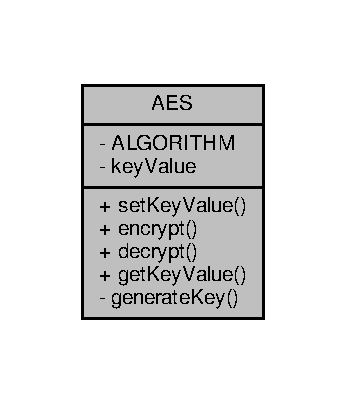
\includegraphics[width=166pt]{a00071}
\end{center}
\end{figure}
\subsection*{Public Member Functions}
\begin{DoxyCompactItemize}
\item 
void \hyperlink{a00001_adac98388bd7c0bf94c3ac2c1987e3f14}{set\+Key\+Value} (byte\mbox{[}$\,$\mbox{]} \hyperlink{a00001_a1a9da325d5376125b139a98e7ff9d2e2}{key\+Value})
\end{DoxyCompactItemize}
\subsection*{Static Public Member Functions}
\begin{DoxyCompactItemize}
\item 
static String \hyperlink{a00001_a4961b27ef3efa77d9ed11ebadffe2c9b}{encrypt} (String data)  throws Exception 
\item 
static String \hyperlink{a00001_a3b7b86cb0a160857d40bd2145364f194}{decrypt} (String encrypted\+Data)  throws Exception 
\item 
static byte\mbox{[}$\,$\mbox{]} \hyperlink{a00001_a2ac0845b551e7ebd2bf47e1beac6df48}{get\+Key\+Value} ()
\end{DoxyCompactItemize}
\subsection*{Static Private Member Functions}
\begin{DoxyCompactItemize}
\item 
static Key \hyperlink{a00001_af920b587f8fd1c20d19b40c110444838}{generate\+Key} ()  throws Exception 
\end{DoxyCompactItemize}
\subsection*{Static Private Attributes}
\begin{DoxyCompactItemize}
\item 
static final String \hyperlink{a00001_a6e0d720a4420fd9bfd6749e43727e4cf}{A\+L\+G\+O\+R\+I\+T\+H\+M} = \char`\"{}A\+E\+S\char`\"{}
\item 
static byte\mbox{[}$\,$\mbox{]} \hyperlink{a00001_a1a9da325d5376125b139a98e7ff9d2e2}{key\+Value}
\end{DoxyCompactItemize}


\subsection{Member Function Documentation}
\hypertarget{a00001_a3b7b86cb0a160857d40bd2145364f194}{\index{org\+::opensecurity\+::sms\+::model\+::security\+::\+A\+E\+S@{org\+::opensecurity\+::sms\+::model\+::security\+::\+A\+E\+S}!decrypt@{decrypt}}
\index{decrypt@{decrypt}!org\+::opensecurity\+::sms\+::model\+::security\+::\+A\+E\+S@{org\+::opensecurity\+::sms\+::model\+::security\+::\+A\+E\+S}}
\subsubsection[{decrypt}]{\setlength{\rightskip}{0pt plus 5cm}static String decrypt (
\begin{DoxyParamCaption}
\item[{String}]{encrypted\+Data}
\end{DoxyParamCaption}
) throws Exception\hspace{0.3cm}{\ttfamily [static]}}}\label{a00001_a3b7b86cb0a160857d40bd2145364f194}
This method decrypts data with \hyperlink{a00001}{A\+E\+S} algorithm using the key of the class


\begin{DoxyParams}{Parameters}
{\em encrypted\+Data} & Data to decrypt \\
\hline
\end{DoxyParams}
\begin{DoxyReturn}{Returns}
Decrypted data 
\end{DoxyReturn}

\begin{DoxyExceptions}{Exceptions}
{\em Exception} & \\
\hline
\end{DoxyExceptions}


Here is the call graph for this function\+:
\nopagebreak
\begin{figure}[H]
\begin{center}
\leavevmode
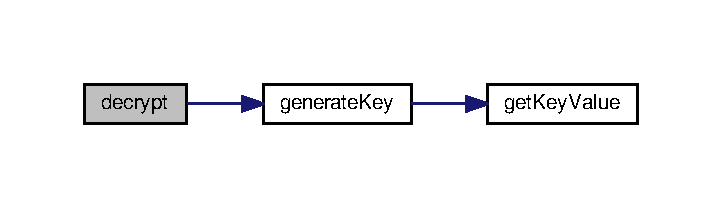
\includegraphics[width=346pt]{a00001_a3b7b86cb0a160857d40bd2145364f194_cgraph}
\end{center}
\end{figure}


\hypertarget{a00001_a4961b27ef3efa77d9ed11ebadffe2c9b}{\index{org\+::opensecurity\+::sms\+::model\+::security\+::\+A\+E\+S@{org\+::opensecurity\+::sms\+::model\+::security\+::\+A\+E\+S}!encrypt@{encrypt}}
\index{encrypt@{encrypt}!org\+::opensecurity\+::sms\+::model\+::security\+::\+A\+E\+S@{org\+::opensecurity\+::sms\+::model\+::security\+::\+A\+E\+S}}
\subsubsection[{encrypt}]{\setlength{\rightskip}{0pt plus 5cm}static String encrypt (
\begin{DoxyParamCaption}
\item[{String}]{data}
\end{DoxyParamCaption}
) throws Exception\hspace{0.3cm}{\ttfamily [static]}}}\label{a00001_a4961b27ef3efa77d9ed11ebadffe2c9b}
This method encrypts data with \hyperlink{a00001}{A\+E\+S} algorithm using the key of the class


\begin{DoxyParams}{Parameters}
{\em data} & Data to encrypt \\
\hline
\end{DoxyParams}
\begin{DoxyReturn}{Returns}
Encrypted data 
\end{DoxyReturn}

\begin{DoxyExceptions}{Exceptions}
{\em Exception} & \\
\hline
\end{DoxyExceptions}


Here is the call graph for this function\+:
\nopagebreak
\begin{figure}[H]
\begin{center}
\leavevmode
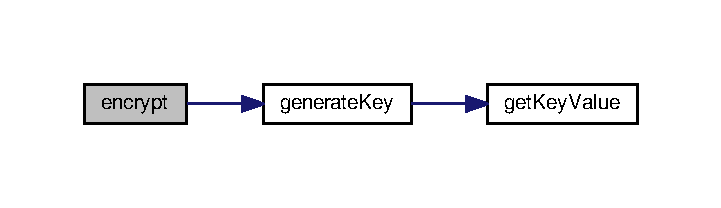
\includegraphics[width=346pt]{a00001_a4961b27ef3efa77d9ed11ebadffe2c9b_cgraph}
\end{center}
\end{figure}


\hypertarget{a00001_af920b587f8fd1c20d19b40c110444838}{\index{org\+::opensecurity\+::sms\+::model\+::security\+::\+A\+E\+S@{org\+::opensecurity\+::sms\+::model\+::security\+::\+A\+E\+S}!generate\+Key@{generate\+Key}}
\index{generate\+Key@{generate\+Key}!org\+::opensecurity\+::sms\+::model\+::security\+::\+A\+E\+S@{org\+::opensecurity\+::sms\+::model\+::security\+::\+A\+E\+S}}
\subsubsection[{generate\+Key}]{\setlength{\rightskip}{0pt plus 5cm}static Key generate\+Key (
\begin{DoxyParamCaption}
{}
\end{DoxyParamCaption}
) throws Exception\hspace{0.3cm}{\ttfamily [static]}, {\ttfamily [private]}}}\label{a00001_af920b587f8fd1c20d19b40c110444838}
This method generates a key with the key value that can be computed with javax.\+crypto method

\begin{DoxyReturn}{Returns}
The key object 
\end{DoxyReturn}

\begin{DoxyExceptions}{Exceptions}
{\em Exception} & \\
\hline
\end{DoxyExceptions}


Here is the call graph for this function\+:
\nopagebreak
\begin{figure}[H]
\begin{center}
\leavevmode
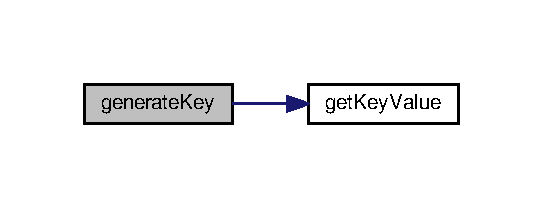
\includegraphics[width=260pt]{a00001_af920b587f8fd1c20d19b40c110444838_cgraph}
\end{center}
\end{figure}




Here is the caller graph for this function\+:
\nopagebreak
\begin{figure}[H]
\begin{center}
\leavevmode
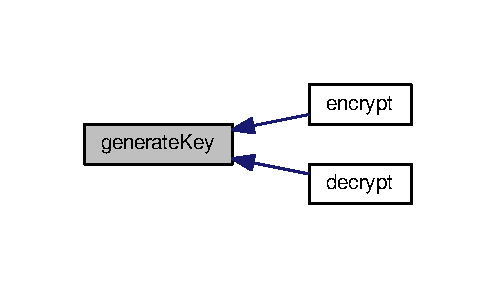
\includegraphics[width=238pt]{a00001_af920b587f8fd1c20d19b40c110444838_icgraph}
\end{center}
\end{figure}


\hypertarget{a00001_a2ac0845b551e7ebd2bf47e1beac6df48}{\index{org\+::opensecurity\+::sms\+::model\+::security\+::\+A\+E\+S@{org\+::opensecurity\+::sms\+::model\+::security\+::\+A\+E\+S}!get\+Key\+Value@{get\+Key\+Value}}
\index{get\+Key\+Value@{get\+Key\+Value}!org\+::opensecurity\+::sms\+::model\+::security\+::\+A\+E\+S@{org\+::opensecurity\+::sms\+::model\+::security\+::\+A\+E\+S}}
\subsubsection[{get\+Key\+Value}]{\setlength{\rightskip}{0pt plus 5cm}static byte \mbox{[}$\,$\mbox{]} get\+Key\+Value (
\begin{DoxyParamCaption}
{}
\end{DoxyParamCaption}
)\hspace{0.3cm}{\ttfamily [static]}}}\label{a00001_a2ac0845b551e7ebd2bf47e1beac6df48}
This method return the key value

\begin{DoxyReturn}{Returns}
The key value 
\end{DoxyReturn}


Here is the caller graph for this function\+:
\nopagebreak
\begin{figure}[H]
\begin{center}
\leavevmode
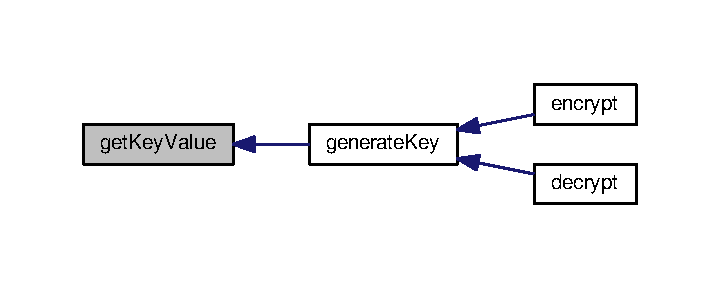
\includegraphics[width=346pt]{a00001_a2ac0845b551e7ebd2bf47e1beac6df48_icgraph}
\end{center}
\end{figure}


\hypertarget{a00001_adac98388bd7c0bf94c3ac2c1987e3f14}{\index{org\+::opensecurity\+::sms\+::model\+::security\+::\+A\+E\+S@{org\+::opensecurity\+::sms\+::model\+::security\+::\+A\+E\+S}!set\+Key\+Value@{set\+Key\+Value}}
\index{set\+Key\+Value@{set\+Key\+Value}!org\+::opensecurity\+::sms\+::model\+::security\+::\+A\+E\+S@{org\+::opensecurity\+::sms\+::model\+::security\+::\+A\+E\+S}}
\subsubsection[{set\+Key\+Value}]{\setlength{\rightskip}{0pt plus 5cm}void set\+Key\+Value (
\begin{DoxyParamCaption}
\item[{byte\mbox{[}$\,$\mbox{]}}]{key\+Value}
\end{DoxyParamCaption}
)}}\label{a00001_adac98388bd7c0bf94c3ac2c1987e3f14}
This method set the key value


\begin{DoxyParams}{Parameters}
{\em key\+Value} & The key value \\
\hline
\end{DoxyParams}


\subsection{Member Data Documentation}
\hypertarget{a00001_a6e0d720a4420fd9bfd6749e43727e4cf}{\index{org\+::opensecurity\+::sms\+::model\+::security\+::\+A\+E\+S@{org\+::opensecurity\+::sms\+::model\+::security\+::\+A\+E\+S}!A\+L\+G\+O\+R\+I\+T\+H\+M@{A\+L\+G\+O\+R\+I\+T\+H\+M}}
\index{A\+L\+G\+O\+R\+I\+T\+H\+M@{A\+L\+G\+O\+R\+I\+T\+H\+M}!org\+::opensecurity\+::sms\+::model\+::security\+::\+A\+E\+S@{org\+::opensecurity\+::sms\+::model\+::security\+::\+A\+E\+S}}
\subsubsection[{A\+L\+G\+O\+R\+I\+T\+H\+M}]{\setlength{\rightskip}{0pt plus 5cm}final String A\+L\+G\+O\+R\+I\+T\+H\+M = \char`\"{}A\+E\+S\char`\"{}\hspace{0.3cm}{\ttfamily [static]}, {\ttfamily [private]}}}\label{a00001_a6e0d720a4420fd9bfd6749e43727e4cf}
\hypertarget{a00001_a1a9da325d5376125b139a98e7ff9d2e2}{\index{org\+::opensecurity\+::sms\+::model\+::security\+::\+A\+E\+S@{org\+::opensecurity\+::sms\+::model\+::security\+::\+A\+E\+S}!key\+Value@{key\+Value}}
\index{key\+Value@{key\+Value}!org\+::opensecurity\+::sms\+::model\+::security\+::\+A\+E\+S@{org\+::opensecurity\+::sms\+::model\+::security\+::\+A\+E\+S}}
\subsubsection[{key\+Value}]{\setlength{\rightskip}{0pt plus 5cm}byte \mbox{[}$\,$\mbox{]} key\+Value\hspace{0.3cm}{\ttfamily [static]}, {\ttfamily [private]}}}\label{a00001_a1a9da325d5376125b139a98e7ff9d2e2}


The documentation for this class was generated from the following file\+:\begin{DoxyCompactItemize}
\item 
app/src/main/java/org/opensecurity/sms/model/security/\hyperlink{a00025}{A\+E\+S.\+java}\end{DoxyCompactItemize}

\hypertarget{a00002}{\section{Array\+Bubble\+Adapter Class Reference}
\label{a00002}\index{Array\+Bubble\+Adapter@{Array\+Bubble\+Adapter}}
}


Inheritance diagram for Array\+Bubble\+Adapter\+:
\nopagebreak
\begin{figure}[H]
\begin{center}
\leavevmode
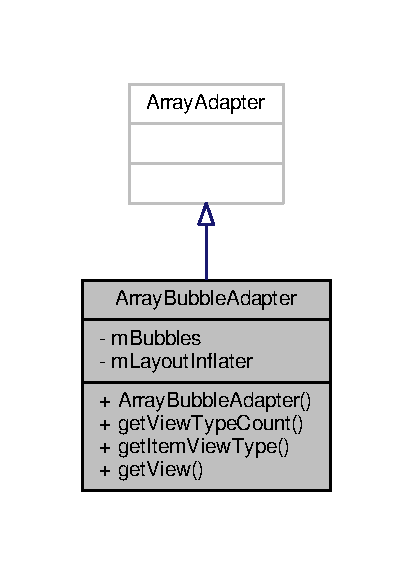
\includegraphics[width=198pt]{a00052}
\end{center}
\end{figure}


Collaboration diagram for Array\+Bubble\+Adapter\+:
\nopagebreak
\begin{figure}[H]
\begin{center}
\leavevmode
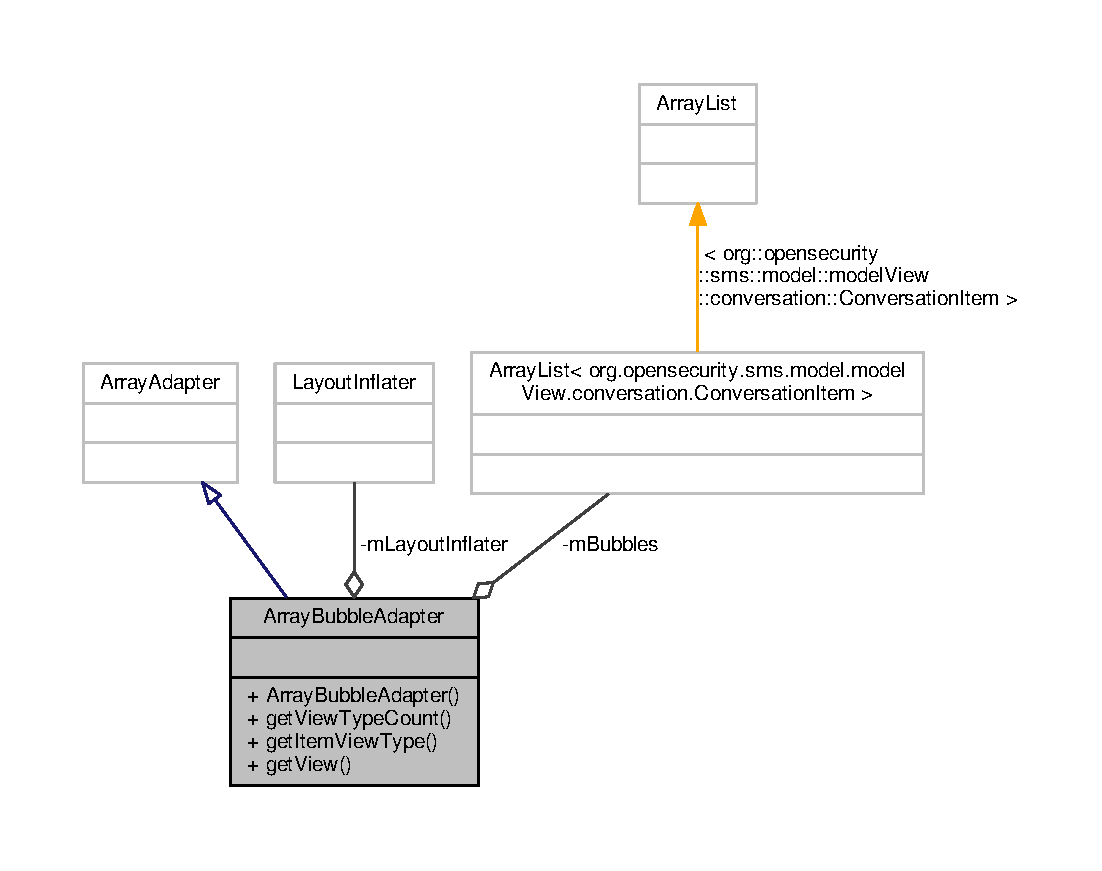
\includegraphics[width=350pt]{a00053}
\end{center}
\end{figure}
\subsection*{Classes}
\begin{DoxyCompactItemize}
\item 
class {\bfseries View\+Holder}
\end{DoxyCompactItemize}
\subsection*{Public Member Functions}
\begin{DoxyCompactItemize}
\item 
\hyperlink{a00002_adbd2cc40c8a00dabffd7b33ef3c7d247}{Array\+Bubble\+Adapter} (Context c, Array\+List$<$ \hyperlink{a00008}{Conversation\+Item} $>$ mb)
\item 
int \hyperlink{a00002_a8085b7d181222b03ef9547a4833ce997}{get\+View\+Type\+Count} ()
\item 
int \hyperlink{a00002_a6d3ccfe62c0e893718ad6266b6207e53}{get\+Item\+View\+Type} (int position)
\item 
View \hyperlink{a00002_af6292d542d7937de5b4044234a2db905}{get\+View} (int position, View convert\+View, View\+Group parent)
\end{DoxyCompactItemize}
\subsection*{Private Attributes}
\begin{DoxyCompactItemize}
\item 
Array\+List$<$ \hyperlink{a00008}{Conversation\+Item} $>$ \hyperlink{a00002_a347536a1eb8525c224f457613e34a80f}{m\+Bubbles}
\item 
Layout\+Inflater \hyperlink{a00002_a4e02ab86d39fcfd990b8dd2f36ccc3c9}{m\+Layout\+Inflater}
\end{DoxyCompactItemize}


\subsection{Detailed Description}
the adapter for displaing the listview of bubbles in a conversation activity 

\subsection{Constructor \& Destructor Documentation}
\hypertarget{a00002_adbd2cc40c8a00dabffd7b33ef3c7d247}{\index{org\+::opensecurity\+::sms\+::model\+::model\+View\+::conversation\+::\+Array\+Bubble\+Adapter@{org\+::opensecurity\+::sms\+::model\+::model\+View\+::conversation\+::\+Array\+Bubble\+Adapter}!Array\+Bubble\+Adapter@{Array\+Bubble\+Adapter}}
\index{Array\+Bubble\+Adapter@{Array\+Bubble\+Adapter}!org\+::opensecurity\+::sms\+::model\+::model\+View\+::conversation\+::\+Array\+Bubble\+Adapter@{org\+::opensecurity\+::sms\+::model\+::model\+View\+::conversation\+::\+Array\+Bubble\+Adapter}}
\subsubsection[{Array\+Bubble\+Adapter}]{\setlength{\rightskip}{0pt plus 5cm}{\bf Array\+Bubble\+Adapter} (
\begin{DoxyParamCaption}
\item[{Context}]{c, }
\item[{Array\+List$<$ {\bf Conversation\+Item} $>$}]{mb}
\end{DoxyParamCaption}
)}}\label{a00002_adbd2cc40c8a00dabffd7b33ef3c7d247}
constructor. 
\begin{DoxyParams}{Parameters}
{\em c} & context interface to global information about an application environment. \\
\hline
{\em mb} & array\+List of bubbles \\
\hline
\end{DoxyParams}


\subsection{Member Function Documentation}
\hypertarget{a00002_a6d3ccfe62c0e893718ad6266b6207e53}{\index{org\+::opensecurity\+::sms\+::model\+::model\+View\+::conversation\+::\+Array\+Bubble\+Adapter@{org\+::opensecurity\+::sms\+::model\+::model\+View\+::conversation\+::\+Array\+Bubble\+Adapter}!get\+Item\+View\+Type@{get\+Item\+View\+Type}}
\index{get\+Item\+View\+Type@{get\+Item\+View\+Type}!org\+::opensecurity\+::sms\+::model\+::model\+View\+::conversation\+::\+Array\+Bubble\+Adapter@{org\+::opensecurity\+::sms\+::model\+::model\+View\+::conversation\+::\+Array\+Bubble\+Adapter}}
\subsubsection[{get\+Item\+View\+Type}]{\setlength{\rightskip}{0pt plus 5cm}int get\+Item\+View\+Type (
\begin{DoxyParamCaption}
\item[{int}]{position}
\end{DoxyParamCaption}
)}}\label{a00002_a6d3ccfe62c0e893718ad6266b6207e53}
to get the current menu type 
\begin{DoxyParams}{Parameters}
{\em position} & the position of selected item \\
\hline
\end{DoxyParams}
\begin{DoxyReturn}{Returns}
the position of selected item 
\end{DoxyReturn}
\hypertarget{a00002_af6292d542d7937de5b4044234a2db905}{\index{org\+::opensecurity\+::sms\+::model\+::model\+View\+::conversation\+::\+Array\+Bubble\+Adapter@{org\+::opensecurity\+::sms\+::model\+::model\+View\+::conversation\+::\+Array\+Bubble\+Adapter}!get\+View@{get\+View}}
\index{get\+View@{get\+View}!org\+::opensecurity\+::sms\+::model\+::model\+View\+::conversation\+::\+Array\+Bubble\+Adapter@{org\+::opensecurity\+::sms\+::model\+::model\+View\+::conversation\+::\+Array\+Bubble\+Adapter}}
\subsubsection[{get\+View}]{\setlength{\rightskip}{0pt plus 5cm}View get\+View (
\begin{DoxyParamCaption}
\item[{int}]{position, }
\item[{View}]{convert\+View, }
\item[{View\+Group}]{parent}
\end{DoxyParamCaption}
)}}\label{a00002_af6292d542d7937de5b4044234a2db905}
get a view that displays the data at the specified position in the data set. This function is called for each rows a bubble contains information loaded thanks to the controller


\begin{DoxyParams}{Parameters}
{\em position} & the position of the item in the listview \\
\hline
{\em convert\+View} & the old view to rescue \\
\hline
{\em parent} & the parent that this view will eventually be attached to (conversation\+Activity) \\
\hline
\end{DoxyParams}
\begin{DoxyReturn}{Returns}
the view of a bubble. Created view by us 
\end{DoxyReturn}
if it's an instance of \hyperlink{a00004}{Bubble}, we create an item with a message\+Body, image\+Bubble etc... Else, We write the date.

Here is the call graph for this function\+:
\nopagebreak
\begin{figure}[H]
\begin{center}
\leavevmode
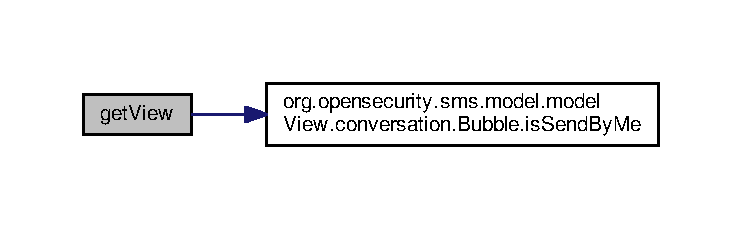
\includegraphics[width=350pt]{a00002_af6292d542d7937de5b4044234a2db905_cgraph}
\end{center}
\end{figure}


\hypertarget{a00002_a8085b7d181222b03ef9547a4833ce997}{\index{org\+::opensecurity\+::sms\+::model\+::model\+View\+::conversation\+::\+Array\+Bubble\+Adapter@{org\+::opensecurity\+::sms\+::model\+::model\+View\+::conversation\+::\+Array\+Bubble\+Adapter}!get\+View\+Type\+Count@{get\+View\+Type\+Count}}
\index{get\+View\+Type\+Count@{get\+View\+Type\+Count}!org\+::opensecurity\+::sms\+::model\+::model\+View\+::conversation\+::\+Array\+Bubble\+Adapter@{org\+::opensecurity\+::sms\+::model\+::model\+View\+::conversation\+::\+Array\+Bubble\+Adapter}}
\subsubsection[{get\+View\+Type\+Count}]{\setlength{\rightskip}{0pt plus 5cm}int get\+View\+Type\+Count (
\begin{DoxyParamCaption}
{}
\end{DoxyParamCaption}
)}}\label{a00002_a8085b7d181222b03ef9547a4833ce997}
to get the number of bubbles in our conversation activity \begin{DoxyReturn}{Returns}
the number of bubbles 
\end{DoxyReturn}


\subsection{Member Data Documentation}
\hypertarget{a00002_a347536a1eb8525c224f457613e34a80f}{\index{org\+::opensecurity\+::sms\+::model\+::model\+View\+::conversation\+::\+Array\+Bubble\+Adapter@{org\+::opensecurity\+::sms\+::model\+::model\+View\+::conversation\+::\+Array\+Bubble\+Adapter}!m\+Bubbles@{m\+Bubbles}}
\index{m\+Bubbles@{m\+Bubbles}!org\+::opensecurity\+::sms\+::model\+::model\+View\+::conversation\+::\+Array\+Bubble\+Adapter@{org\+::opensecurity\+::sms\+::model\+::model\+View\+::conversation\+::\+Array\+Bubble\+Adapter}}
\subsubsection[{m\+Bubbles}]{\setlength{\rightskip}{0pt plus 5cm}Array\+List$<${\bf Conversation\+Item}$>$ m\+Bubbles\hspace{0.3cm}{\ttfamily [private]}}}\label{a00002_a347536a1eb8525c224f457613e34a80f}
the bubbles of our conversation in a array\+List \hypertarget{a00002_a4e02ab86d39fcfd990b8dd2f36ccc3c9}{\index{org\+::opensecurity\+::sms\+::model\+::model\+View\+::conversation\+::\+Array\+Bubble\+Adapter@{org\+::opensecurity\+::sms\+::model\+::model\+View\+::conversation\+::\+Array\+Bubble\+Adapter}!m\+Layout\+Inflater@{m\+Layout\+Inflater}}
\index{m\+Layout\+Inflater@{m\+Layout\+Inflater}!org\+::opensecurity\+::sms\+::model\+::model\+View\+::conversation\+::\+Array\+Bubble\+Adapter@{org\+::opensecurity\+::sms\+::model\+::model\+View\+::conversation\+::\+Array\+Bubble\+Adapter}}
\subsubsection[{m\+Layout\+Inflater}]{\setlength{\rightskip}{0pt plus 5cm}Layout\+Inflater m\+Layout\+Inflater\hspace{0.3cm}{\ttfamily [private]}}}\label{a00002_a4e02ab86d39fcfd990b8dd2f36ccc3c9}
to instantiates a layout X\+M\+L file into its corresponding view objects 

The documentation for this class was generated from the following file\+:\begin{DoxyCompactItemize}
\item 
app/src/main/java/org/opensecurity/sms/model/model\+View/conversation/\hyperlink{a00018}{Array\+Bubble\+Adapter.\+java}\end{DoxyCompactItemize}

\hypertarget{a00003}{\section{Array\+Convers\+Adapter Class Reference}
\label{a00003}\index{Array\+Convers\+Adapter@{Array\+Convers\+Adapter}}
}


Inheritance diagram for Array\+Convers\+Adapter\+:
\nopagebreak
\begin{figure}[H]
\begin{center}
\leavevmode
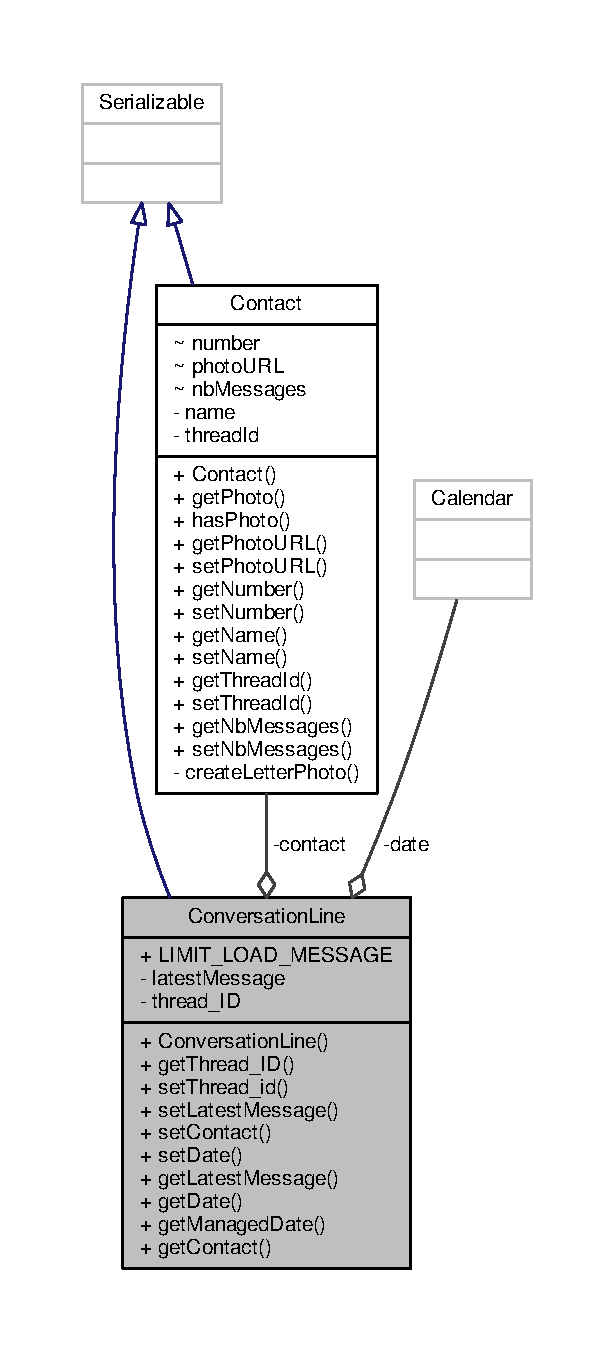
\includegraphics[width=204pt]{a00065}
\end{center}
\end{figure}


Collaboration diagram for Array\+Convers\+Adapter\+:
\nopagebreak
\begin{figure}[H]
\begin{center}
\leavevmode
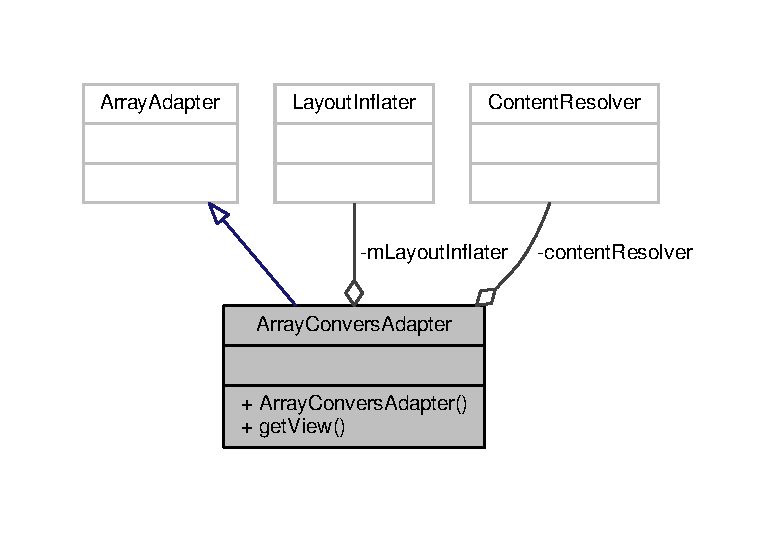
\includegraphics[width=350pt]{a00066}
\end{center}
\end{figure}
\subsection*{Classes}
\begin{DoxyCompactItemize}
\item 
class {\bfseries View\+Holder}
\end{DoxyCompactItemize}
\subsection*{Public Member Functions}
\begin{DoxyCompactItemize}
\item 
\hyperlink{a00003_a6c4aeef04be96ad661e6cb67f4f192cf}{Array\+Convers\+Adapter} (Context context, List$<$ \hyperlink{a00008}{Conversation\+Line} $>$ rep)
\item 
View \hyperlink{a00003_af6292d542d7937de5b4044234a2db905}{get\+View} (int position, View convert\+View, View\+Group parent)
\end{DoxyCompactItemize}
\subsection*{Private Attributes}
\begin{DoxyCompactItemize}
\item 
Layout\+Inflater \hyperlink{a00003_a4e02ab86d39fcfd990b8dd2f36ccc3c9}{m\+Layout\+Inflater}
\item 
Content\+Resolver \hyperlink{a00003_a261822b570bfffa0c90ead212414c9b6}{content\+Resolver}
\end{DoxyCompactItemize}


\subsection{Detailed Description}
This class is used to set an adapter of a list of conversation (in the main activity) it's a child of Array\+Adapter. 

\subsection{Constructor \& Destructor Documentation}
\hypertarget{a00003_a6c4aeef04be96ad661e6cb67f4f192cf}{\index{org\+::opensecurity\+::sms\+::model\+::model\+View\+::list\+Conversation\+::\+Array\+Convers\+Adapter@{org\+::opensecurity\+::sms\+::model\+::model\+View\+::list\+Conversation\+::\+Array\+Convers\+Adapter}!Array\+Convers\+Adapter@{Array\+Convers\+Adapter}}
\index{Array\+Convers\+Adapter@{Array\+Convers\+Adapter}!org\+::opensecurity\+::sms\+::model\+::model\+View\+::list\+Conversation\+::\+Array\+Convers\+Adapter@{org\+::opensecurity\+::sms\+::model\+::model\+View\+::list\+Conversation\+::\+Array\+Convers\+Adapter}}
\subsubsection[{Array\+Convers\+Adapter}]{\setlength{\rightskip}{0pt plus 5cm}{\bf Array\+Convers\+Adapter} (
\begin{DoxyParamCaption}
\item[{Context}]{context, }
\item[{List$<$ {\bf Conversation\+Line} $>$}]{rep}
\end{DoxyParamCaption}
)}}\label{a00003_a6c4aeef04be96ad661e6cb67f4f192cf}

\begin{DoxyParams}{Parameters}
{\em context} & \\
\hline
{\em rep} & \\
\hline
\end{DoxyParams}


\subsection{Member Function Documentation}
\hypertarget{a00003_af6292d542d7937de5b4044234a2db905}{\index{org\+::opensecurity\+::sms\+::model\+::model\+View\+::list\+Conversation\+::\+Array\+Convers\+Adapter@{org\+::opensecurity\+::sms\+::model\+::model\+View\+::list\+Conversation\+::\+Array\+Convers\+Adapter}!get\+View@{get\+View}}
\index{get\+View@{get\+View}!org\+::opensecurity\+::sms\+::model\+::model\+View\+::list\+Conversation\+::\+Array\+Convers\+Adapter@{org\+::opensecurity\+::sms\+::model\+::model\+View\+::list\+Conversation\+::\+Array\+Convers\+Adapter}}
\subsubsection[{get\+View}]{\setlength{\rightskip}{0pt plus 5cm}View get\+View (
\begin{DoxyParamCaption}
\item[{int}]{position, }
\item[{View}]{convert\+View, }
\item[{View\+Group}]{parent}
\end{DoxyParamCaption}
)}}\label{a00003_af6292d542d7937de5b4044234a2db905}
position \+: position in the list of conversations.. convert\+View \+: given by the system to recycle or recalculate row\+View wich has just appeared (by scrolling for example)

permet la récupération de la vue personnalisée d'une ligne (row\+View) qui contiendra, grâce au X\+M\+L, nos deux élements de textes que nous pourront exploiter afin de pouvoir y personnaliser. La méthode get\+View est appelée pour générer chaque lignes de l'écran.

This method is a redefinition of get\+View in class Array\+Adapter witch is used for calculate one element of our list of widget row\+View created by us. permit the recycling (or calculate) and return the personalized view of a line (row\+View) witch will be composed of, thanks to X\+M\+L, tow entities of the Text\+View. (ref to R.\+layout.\+listofconvers.\+xml) this method is called every time the program need to generate a rowview.

If you want to improve the design of the list\+Of\+Convers activity (main activity) refer to R.\+layout.\+listofconvers.\+xml and R.\+layout.\+opensecuritysms.\+xml get a view that displays the data at the specified position in the data set. This function is called for each rows a row contains information loaded thanks to the controller


\begin{DoxyParams}{Parameters}
{\em position} & the position of the item in the listview \\
\hline
{\em convert\+View} & the old view to rescue \\
\hline
{\em parent} & the parent that this view will eventually be attached to (main\+Activity) \\
\hline
\end{DoxyParams}
\begin{DoxyReturn}{Returns}
the view of a row. Created view by us 
\end{DoxyReturn}


\subsection{Member Data Documentation}
\hypertarget{a00003_a261822b570bfffa0c90ead212414c9b6}{\index{org\+::opensecurity\+::sms\+::model\+::model\+View\+::list\+Conversation\+::\+Array\+Convers\+Adapter@{org\+::opensecurity\+::sms\+::model\+::model\+View\+::list\+Conversation\+::\+Array\+Convers\+Adapter}!content\+Resolver@{content\+Resolver}}
\index{content\+Resolver@{content\+Resolver}!org\+::opensecurity\+::sms\+::model\+::model\+View\+::list\+Conversation\+::\+Array\+Convers\+Adapter@{org\+::opensecurity\+::sms\+::model\+::model\+View\+::list\+Conversation\+::\+Array\+Convers\+Adapter}}
\subsubsection[{content\+Resolver}]{\setlength{\rightskip}{0pt plus 5cm}Content\+Resolver content\+Resolver\hspace{0.3cm}{\ttfamily [private]}}}\label{a00003_a261822b570bfffa0c90ead212414c9b6}
\hypertarget{a00003_a4e02ab86d39fcfd990b8dd2f36ccc3c9}{\index{org\+::opensecurity\+::sms\+::model\+::model\+View\+::list\+Conversation\+::\+Array\+Convers\+Adapter@{org\+::opensecurity\+::sms\+::model\+::model\+View\+::list\+Conversation\+::\+Array\+Convers\+Adapter}!m\+Layout\+Inflater@{m\+Layout\+Inflater}}
\index{m\+Layout\+Inflater@{m\+Layout\+Inflater}!org\+::opensecurity\+::sms\+::model\+::model\+View\+::list\+Conversation\+::\+Array\+Convers\+Adapter@{org\+::opensecurity\+::sms\+::model\+::model\+View\+::list\+Conversation\+::\+Array\+Convers\+Adapter}}
\subsubsection[{m\+Layout\+Inflater}]{\setlength{\rightskip}{0pt plus 5cm}Layout\+Inflater m\+Layout\+Inflater\hspace{0.3cm}{\ttfamily [private]}}}\label{a00003_a4e02ab86d39fcfd990b8dd2f36ccc3c9}


The documentation for this class was generated from the following file\+:\begin{DoxyCompactItemize}
\item 
app/src/main/java/org/opensecurity/sms/model/model\+View/list\+Conversation/\hyperlink{a00023}{Array\+Convers\+Adapter.\+java}\end{DoxyCompactItemize}

\hypertarget{a00004}{\section{Bubble Class Reference}
\label{a00004}\index{Bubble@{Bubble}}
}


Inheritance diagram for Bubble\+:
\nopagebreak
\begin{figure}[H]
\begin{center}
\leavevmode
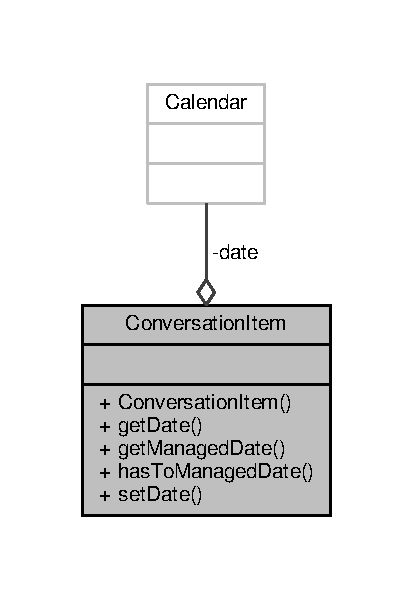
\includegraphics[width=198pt]{a00059}
\end{center}
\end{figure}


Collaboration diagram for Bubble\+:
\nopagebreak
\begin{figure}[H]
\begin{center}
\leavevmode
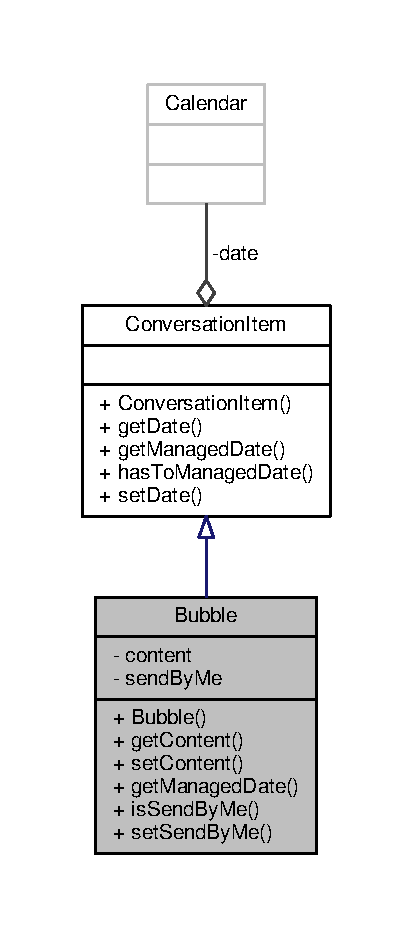
\includegraphics[width=198pt]{a00060}
\end{center}
\end{figure}
\subsection*{Public Member Functions}
\begin{DoxyCompactItemize}
\item 
\hyperlink{a00004_a3c1c7b516864bb50a824afc262da30ce}{Bubble} (String \hyperlink{a00004_a5afce1c98d73512f8ffcb0482df23708}{content}, Calendar \hyperlink{a00007_aa713d1025d73543bd4eae313a1868570}{date}, boolean \hyperlink{a00004_a87564ae3e1ae394e9b16de538dbf8067}{send\+By\+Me})
\item 
String \hyperlink{a00004_ab19dc9b592b32a2db1af785e9083d0e5}{get\+Content} ()
\item 
void \hyperlink{a00004_a31abdf74d2b9d2afe2db6c12c6451501}{set\+Content} (String \hyperlink{a00004_a5afce1c98d73512f8ffcb0482df23708}{content})
\item 
String \hyperlink{a00004_aa53441954dd0352c8b8964194365c688}{get\+Managed\+Date} ()
\item 
boolean \hyperlink{a00004_a0506f5775946d7c4db49b611d57fa3da}{is\+Send\+By\+Me} ()
\item 
void \hyperlink{a00004_a10871b9b5592dcf11e26eaed8e407682}{set\+Send\+By\+Me} (boolean \hyperlink{a00004_a87564ae3e1ae394e9b16de538dbf8067}{send\+By\+Me})
\end{DoxyCompactItemize}
\subsection*{Private Attributes}
\begin{DoxyCompactItemize}
\item 
String \hyperlink{a00004_a5afce1c98d73512f8ffcb0482df23708}{content}
\item 
boolean \hyperlink{a00004_a87564ae3e1ae394e9b16de538dbf8067}{send\+By\+Me}
\end{DoxyCompactItemize}


\subsection{Detailed Description}
class bubble. On of conversation\+Item. Possible row in a conversation\+Activity. 

\subsection{Constructor \& Destructor Documentation}
\hypertarget{a00004_a3c1c7b516864bb50a824afc262da30ce}{\index{org\+::opensecurity\+::sms\+::model\+::model\+View\+::conversation\+::\+Bubble@{org\+::opensecurity\+::sms\+::model\+::model\+View\+::conversation\+::\+Bubble}!Bubble@{Bubble}}
\index{Bubble@{Bubble}!org\+::opensecurity\+::sms\+::model\+::model\+View\+::conversation\+::\+Bubble@{org\+::opensecurity\+::sms\+::model\+::model\+View\+::conversation\+::\+Bubble}}
\subsubsection[{Bubble}]{\setlength{\rightskip}{0pt plus 5cm}{\bf Bubble} (
\begin{DoxyParamCaption}
\item[{String}]{content, }
\item[{Calendar}]{date, }
\item[{boolean}]{send\+By\+Me}
\end{DoxyParamCaption}
)}}\label{a00004_a3c1c7b516864bb50a824afc262da30ce}
Constructor


\begin{DoxyParams}{Parameters}
{\em content} & The content of the bubble \\
\hline
{\em date} & The date of reception of the message \\
\hline
{\em send\+By\+Me} & True if send by the phone, False if not \\
\hline
\end{DoxyParams}


Here is the call graph for this function\+:\nopagebreak
\begin{figure}[H]
\begin{center}
\leavevmode
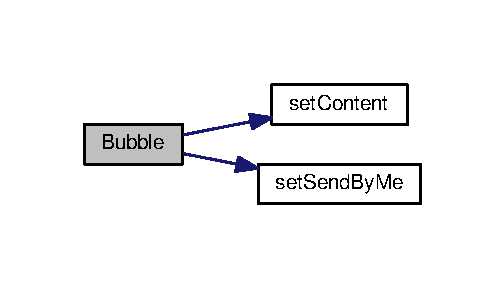
\includegraphics[width=242pt]{a00004_a3c1c7b516864bb50a824afc262da30ce_cgraph}
\end{center}
\end{figure}




\subsection{Member Function Documentation}
\hypertarget{a00004_ab19dc9b592b32a2db1af785e9083d0e5}{\index{org\+::opensecurity\+::sms\+::model\+::model\+View\+::conversation\+::\+Bubble@{org\+::opensecurity\+::sms\+::model\+::model\+View\+::conversation\+::\+Bubble}!get\+Content@{get\+Content}}
\index{get\+Content@{get\+Content}!org\+::opensecurity\+::sms\+::model\+::model\+View\+::conversation\+::\+Bubble@{org\+::opensecurity\+::sms\+::model\+::model\+View\+::conversation\+::\+Bubble}}
\subsubsection[{get\+Content}]{\setlength{\rightskip}{0pt plus 5cm}String get\+Content (
\begin{DoxyParamCaption}
{}
\end{DoxyParamCaption}
)}}\label{a00004_ab19dc9b592b32a2db1af785e9083d0e5}
This method returns the content of the bubble

\begin{DoxyReturn}{Returns}
The content of the bubble 
\end{DoxyReturn}
\hypertarget{a00004_aa53441954dd0352c8b8964194365c688}{\index{org\+::opensecurity\+::sms\+::model\+::model\+View\+::conversation\+::\+Bubble@{org\+::opensecurity\+::sms\+::model\+::model\+View\+::conversation\+::\+Bubble}!get\+Managed\+Date@{get\+Managed\+Date}}
\index{get\+Managed\+Date@{get\+Managed\+Date}!org\+::opensecurity\+::sms\+::model\+::model\+View\+::conversation\+::\+Bubble@{org\+::opensecurity\+::sms\+::model\+::model\+View\+::conversation\+::\+Bubble}}
\subsubsection[{get\+Managed\+Date}]{\setlength{\rightskip}{0pt plus 5cm}String get\+Managed\+Date (
\begin{DoxyParamCaption}
{}
\end{DoxyParamCaption}
)}}\label{a00004_aa53441954dd0352c8b8964194365c688}
This method computes the date in a human readable format using hours and minutes.

\begin{DoxyReturn}{Returns}
The human readable date 
\end{DoxyReturn}


Here is the call graph for this function\+:
\nopagebreak
\begin{figure}[H]
\begin{center}
\leavevmode
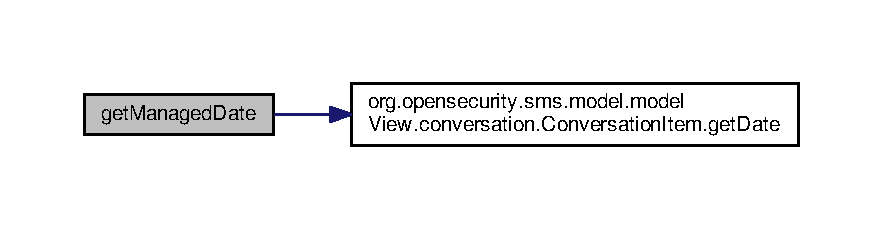
\includegraphics[width=350pt]{a00004_aa53441954dd0352c8b8964194365c688_cgraph}
\end{center}
\end{figure}


\hypertarget{a00004_a0506f5775946d7c4db49b611d57fa3da}{\index{org\+::opensecurity\+::sms\+::model\+::model\+View\+::conversation\+::\+Bubble@{org\+::opensecurity\+::sms\+::model\+::model\+View\+::conversation\+::\+Bubble}!is\+Send\+By\+Me@{is\+Send\+By\+Me}}
\index{is\+Send\+By\+Me@{is\+Send\+By\+Me}!org\+::opensecurity\+::sms\+::model\+::model\+View\+::conversation\+::\+Bubble@{org\+::opensecurity\+::sms\+::model\+::model\+View\+::conversation\+::\+Bubble}}
\subsubsection[{is\+Send\+By\+Me}]{\setlength{\rightskip}{0pt plus 5cm}boolean is\+Send\+By\+Me (
\begin{DoxyParamCaption}
{}
\end{DoxyParamCaption}
)}}\label{a00004_a0506f5775946d7c4db49b611d57fa3da}
This method returns True if the message was sent by the phone, False if not

\begin{DoxyReturn}{Returns}
True if the message was sent by the phone, False if not 
\end{DoxyReturn}


Here is the caller graph for this function\+:\nopagebreak
\begin{figure}[H]
\begin{center}
\leavevmode
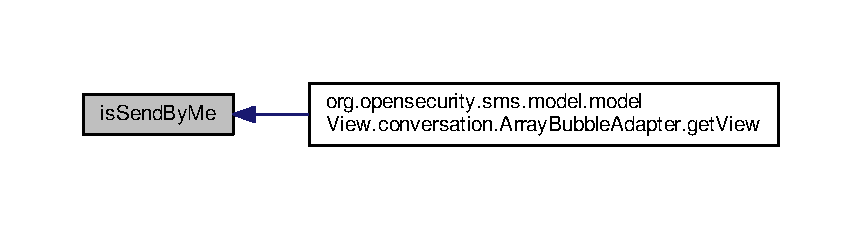
\includegraphics[width=350pt]{a00004_a0506f5775946d7c4db49b611d57fa3da_icgraph}
\end{center}
\end{figure}


\hypertarget{a00004_a31abdf74d2b9d2afe2db6c12c6451501}{\index{org\+::opensecurity\+::sms\+::model\+::model\+View\+::conversation\+::\+Bubble@{org\+::opensecurity\+::sms\+::model\+::model\+View\+::conversation\+::\+Bubble}!set\+Content@{set\+Content}}
\index{set\+Content@{set\+Content}!org\+::opensecurity\+::sms\+::model\+::model\+View\+::conversation\+::\+Bubble@{org\+::opensecurity\+::sms\+::model\+::model\+View\+::conversation\+::\+Bubble}}
\subsubsection[{set\+Content}]{\setlength{\rightskip}{0pt plus 5cm}void set\+Content (
\begin{DoxyParamCaption}
\item[{String}]{content}
\end{DoxyParamCaption}
)}}\label{a00004_a31abdf74d2b9d2afe2db6c12c6451501}
This method set the content of the bubble


\begin{DoxyParams}{Parameters}
{\em content} & The content of the bubble \\
\hline
\end{DoxyParams}


Here is the caller graph for this function\+:\nopagebreak
\begin{figure}[H]
\begin{center}
\leavevmode
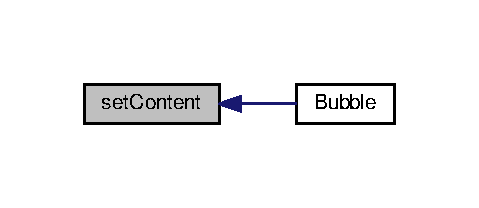
\includegraphics[width=230pt]{a00004_a31abdf74d2b9d2afe2db6c12c6451501_icgraph}
\end{center}
\end{figure}


\hypertarget{a00004_a10871b9b5592dcf11e26eaed8e407682}{\index{org\+::opensecurity\+::sms\+::model\+::model\+View\+::conversation\+::\+Bubble@{org\+::opensecurity\+::sms\+::model\+::model\+View\+::conversation\+::\+Bubble}!set\+Send\+By\+Me@{set\+Send\+By\+Me}}
\index{set\+Send\+By\+Me@{set\+Send\+By\+Me}!org\+::opensecurity\+::sms\+::model\+::model\+View\+::conversation\+::\+Bubble@{org\+::opensecurity\+::sms\+::model\+::model\+View\+::conversation\+::\+Bubble}}
\subsubsection[{set\+Send\+By\+Me}]{\setlength{\rightskip}{0pt plus 5cm}void set\+Send\+By\+Me (
\begin{DoxyParamCaption}
\item[{boolean}]{send\+By\+Me}
\end{DoxyParamCaption}
)}}\label{a00004_a10871b9b5592dcf11e26eaed8e407682}
This method sets the boolean send\+By\+Me


\begin{DoxyParams}{Parameters}
{\em send\+By\+Me} & The message status \\
\hline
\end{DoxyParams}


Here is the caller graph for this function\+:\nopagebreak
\begin{figure}[H]
\begin{center}
\leavevmode
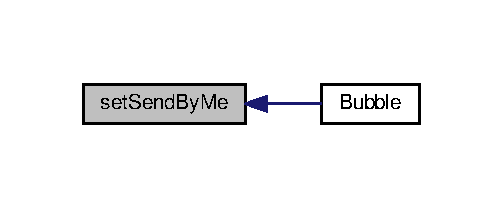
\includegraphics[width=242pt]{a00004_a10871b9b5592dcf11e26eaed8e407682_icgraph}
\end{center}
\end{figure}




\subsection{Member Data Documentation}
\hypertarget{a00004_a5afce1c98d73512f8ffcb0482df23708}{\index{org\+::opensecurity\+::sms\+::model\+::model\+View\+::conversation\+::\+Bubble@{org\+::opensecurity\+::sms\+::model\+::model\+View\+::conversation\+::\+Bubble}!content@{content}}
\index{content@{content}!org\+::opensecurity\+::sms\+::model\+::model\+View\+::conversation\+::\+Bubble@{org\+::opensecurity\+::sms\+::model\+::model\+View\+::conversation\+::\+Bubble}}
\subsubsection[{content}]{\setlength{\rightskip}{0pt plus 5cm}String content\hspace{0.3cm}{\ttfamily [private]}}}\label{a00004_a5afce1c98d73512f8ffcb0482df23708}
the text into a conversation\+Item \hypertarget{a00004_a87564ae3e1ae394e9b16de538dbf8067}{\index{org\+::opensecurity\+::sms\+::model\+::model\+View\+::conversation\+::\+Bubble@{org\+::opensecurity\+::sms\+::model\+::model\+View\+::conversation\+::\+Bubble}!send\+By\+Me@{send\+By\+Me}}
\index{send\+By\+Me@{send\+By\+Me}!org\+::opensecurity\+::sms\+::model\+::model\+View\+::conversation\+::\+Bubble@{org\+::opensecurity\+::sms\+::model\+::model\+View\+::conversation\+::\+Bubble}}
\subsubsection[{send\+By\+Me}]{\setlength{\rightskip}{0pt plus 5cm}boolean send\+By\+Me\hspace{0.3cm}{\ttfamily [private]}}}\label{a00004_a87564ae3e1ae394e9b16de538dbf8067}
true if it's a message send by me. False if not 

The documentation for this class was generated from the following file\+:\begin{DoxyCompactItemize}
\item 
app/src/main/java/org/opensecurity/sms/model/model\+View/conversation/\hyperlink{a00021}{Bubble.\+java}\end{DoxyCompactItemize}

\hypertarget{a00005}{\section{Contact Class Reference}
\label{a00005}\index{Contact@{Contact}}
}


Inheritance diagram for Contact\+:
\nopagebreak
\begin{figure}[H]
\begin{center}
\leavevmode
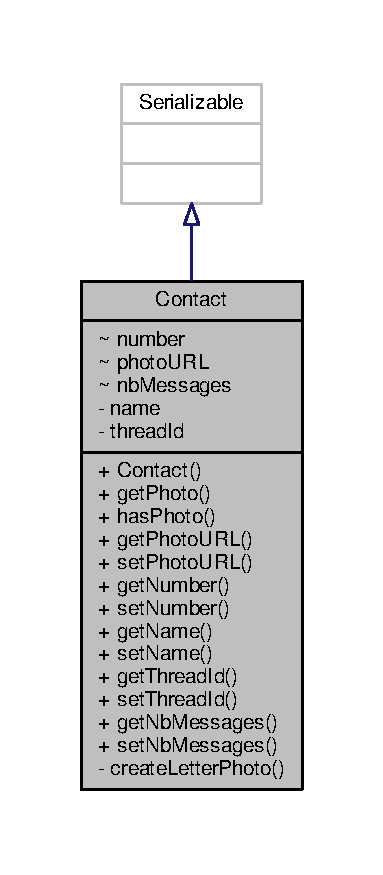
\includegraphics[width=184pt]{a00043}
\end{center}
\end{figure}


Collaboration diagram for Contact\+:
\nopagebreak
\begin{figure}[H]
\begin{center}
\leavevmode
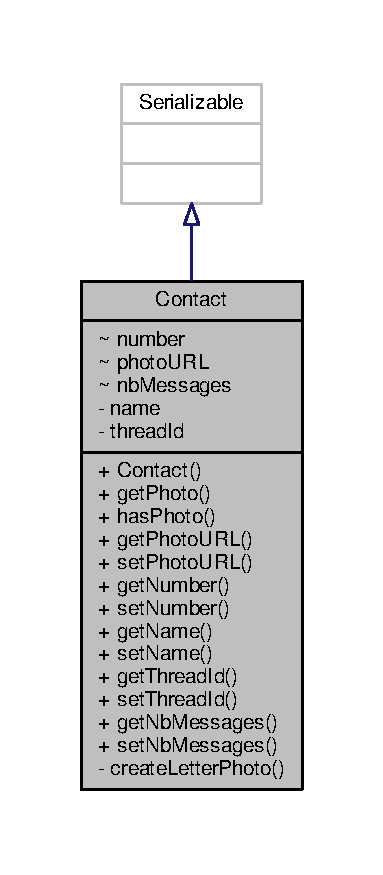
\includegraphics[width=184pt]{a00044}
\end{center}
\end{figure}
\subsection*{Public Member Functions}
\begin{DoxyCompactItemize}
\item 
\hyperlink{a00005_a338f8ea370a08d4566739c2950bf1bd7}{Contact} (String \hyperlink{a00005_a59be7928addfd6c2307fa665d9d0eb3a}{number})
\item 
final Bitmap \hyperlink{a00005_a589071d4450e576bcf705b147a5d8dfc}{get\+Photo} (Content\+Resolver content\+Resolver)
\item 
boolean \hyperlink{a00005_a6f861ae47c26fefab4e8e0cea9a1c979}{has\+Photo} ()
\item 
String \hyperlink{a00005_acb254f588afdb1371b7fcf708e8e665d}{get\+Photo\+U\+R\+L} ()
\item 
void \hyperlink{a00005_a26188abec636b2754749851d108157c9}{set\+Photo\+U\+R\+L} (String \hyperlink{a00005_a6300d0c52298ebf7049df45c04ca1879}{photo\+U\+R\+L})
\item 
String \hyperlink{a00005_ae03bcf255a5fc2f7d29438a9a310144e}{get\+Number} ()
\item 
void \hyperlink{a00005_a5248a434af8755dc41918e83e8cbe2cc}{set\+Number} (String \hyperlink{a00005_a59be7928addfd6c2307fa665d9d0eb3a}{number})
\item 
String \hyperlink{a00005_a78ee178b6a73658d65ca60da4d1e6683}{get\+Name} ()
\item 
void \hyperlink{a00005_ad737b36b74be994e0d8420797ed72f78}{set\+Name} (String \hyperlink{a00005_a9a2326f35466e54c36c070829245c557}{name})
\item 
int \hyperlink{a00005_ad0e00784944089a9ece0934817c8976b}{get\+Thread\+Id} ()
\item 
void \hyperlink{a00005_a0d24ce5a0d8f054366321a58db5d4d0a}{set\+Thread\+Id} (int \hyperlink{a00005_afdf9018750ccb340d2173b2a3da1e755}{thread\+Id})
\item 
int \hyperlink{a00005_ab2e6122640650f7b784fabadd00f823a}{get\+Nb\+Messages} ()
\item 
void \hyperlink{a00005_a5bad44419074a927bf68c94245f36890}{set\+Nb\+Messages} (int \hyperlink{a00005_a88c965ed9f3385173d81f6bd02caac09}{nb\+Messages})
\end{DoxyCompactItemize}
\subsection*{Package Attributes}
\begin{DoxyCompactItemize}
\item 
String \hyperlink{a00005_a59be7928addfd6c2307fa665d9d0eb3a}{number}
\item 
String \hyperlink{a00005_a6300d0c52298ebf7049df45c04ca1879}{photo\+U\+R\+L}
\item 
int \hyperlink{a00005_a88c965ed9f3385173d81f6bd02caac09}{nb\+Messages}
\end{DoxyCompactItemize}
\subsection*{Private Member Functions}
\begin{DoxyCompactItemize}
\item 
final Bitmap \hyperlink{a00005_af33120ef9b221b960200352a7f202631}{create\+Letter\+Photo} ()
\end{DoxyCompactItemize}
\subsection*{Private Attributes}
\begin{DoxyCompactItemize}
\item 
String \hyperlink{a00005_a9a2326f35466e54c36c070829245c557}{name}
\item 
int \hyperlink{a00005_afdf9018750ccb340d2173b2a3da1e755}{thread\+Id}
\end{DoxyCompactItemize}


\subsection{Detailed Description}
The contact class. An object Created by Valentin on 10/11/2015. 

\subsection{Constructor \& Destructor Documentation}
\hypertarget{a00005_a338f8ea370a08d4566739c2950bf1bd7}{\index{org\+::opensecurity\+::sms\+::model\+::\+Contact@{org\+::opensecurity\+::sms\+::model\+::\+Contact}!Contact@{Contact}}
\index{Contact@{Contact}!org\+::opensecurity\+::sms\+::model\+::\+Contact@{org\+::opensecurity\+::sms\+::model\+::\+Contact}}
\subsubsection[{Contact}]{\setlength{\rightskip}{0pt plus 5cm}{\bf Contact} (
\begin{DoxyParamCaption}
\item[{String}]{number}
\end{DoxyParamCaption}
)}}\label{a00005_a338f8ea370a08d4566739c2950bf1bd7}
constructor 
\begin{DoxyParams}{Parameters}
{\em number} & his phone\+Number \\
\hline
\end{DoxyParams}


Here is the call graph for this function\+:
\nopagebreak
\begin{figure}[H]
\begin{center}
\leavevmode
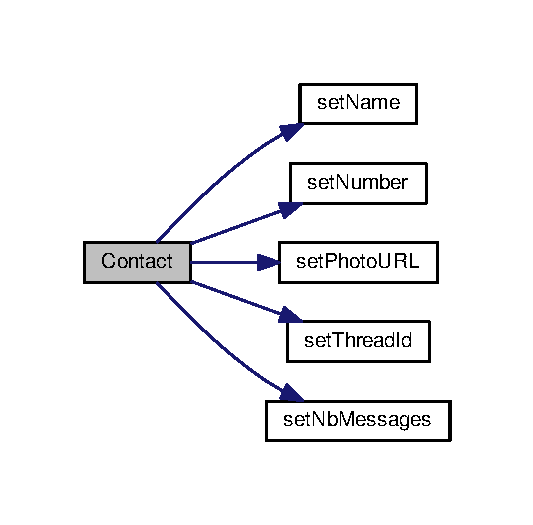
\includegraphics[width=256pt]{a00005_a338f8ea370a08d4566739c2950bf1bd7_cgraph}
\end{center}
\end{figure}




\subsection{Member Function Documentation}
\hypertarget{a00005_af33120ef9b221b960200352a7f202631}{\index{org\+::opensecurity\+::sms\+::model\+::\+Contact@{org\+::opensecurity\+::sms\+::model\+::\+Contact}!create\+Letter\+Photo@{create\+Letter\+Photo}}
\index{create\+Letter\+Photo@{create\+Letter\+Photo}!org\+::opensecurity\+::sms\+::model\+::\+Contact@{org\+::opensecurity\+::sms\+::model\+::\+Contact}}
\subsubsection[{create\+Letter\+Photo}]{\setlength{\rightskip}{0pt plus 5cm}final Bitmap create\+Letter\+Photo (
\begin{DoxyParamCaption}
{}
\end{DoxyParamCaption}
)\hspace{0.3cm}{\ttfamily [private]}}}\label{a00005_af33120ef9b221b960200352a7f202631}
to create letter on a picture if we havn't the picture for our contact \begin{DoxyReturn}{Returns}
bitmap picture of our contact 
\end{DoxyReturn}


Here is the call graph for this function\+:
\nopagebreak
\begin{figure}[H]
\begin{center}
\leavevmode
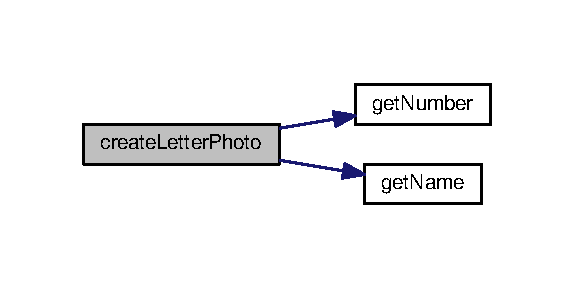
\includegraphics[width=276pt]{a00005_af33120ef9b221b960200352a7f202631_cgraph}
\end{center}
\end{figure}




Here is the caller graph for this function\+:
\nopagebreak
\begin{figure}[H]
\begin{center}
\leavevmode
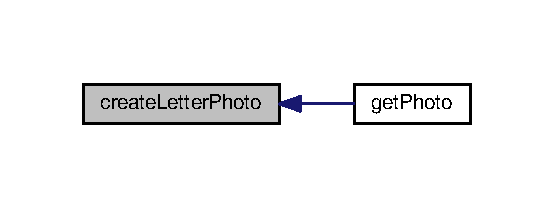
\includegraphics[width=266pt]{a00005_af33120ef9b221b960200352a7f202631_icgraph}
\end{center}
\end{figure}


\hypertarget{a00005_a78ee178b6a73658d65ca60da4d1e6683}{\index{org\+::opensecurity\+::sms\+::model\+::\+Contact@{org\+::opensecurity\+::sms\+::model\+::\+Contact}!get\+Name@{get\+Name}}
\index{get\+Name@{get\+Name}!org\+::opensecurity\+::sms\+::model\+::\+Contact@{org\+::opensecurity\+::sms\+::model\+::\+Contact}}
\subsubsection[{get\+Name}]{\setlength{\rightskip}{0pt plus 5cm}String get\+Name (
\begin{DoxyParamCaption}
{}
\end{DoxyParamCaption}
)}}\label{a00005_a78ee178b6a73658d65ca60da4d1e6683}
to get the name of current contact \begin{DoxyReturn}{Returns}
the name of the current contact 
\end{DoxyReturn}


Here is the caller graph for this function\+:
\nopagebreak
\begin{figure}[H]
\begin{center}
\leavevmode
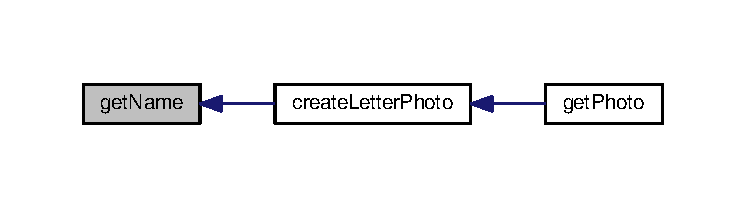
\includegraphics[width=350pt]{a00005_a78ee178b6a73658d65ca60da4d1e6683_icgraph}
\end{center}
\end{figure}


\hypertarget{a00005_ab2e6122640650f7b784fabadd00f823a}{\index{org\+::opensecurity\+::sms\+::model\+::\+Contact@{org\+::opensecurity\+::sms\+::model\+::\+Contact}!get\+Nb\+Messages@{get\+Nb\+Messages}}
\index{get\+Nb\+Messages@{get\+Nb\+Messages}!org\+::opensecurity\+::sms\+::model\+::\+Contact@{org\+::opensecurity\+::sms\+::model\+::\+Contact}}
\subsubsection[{get\+Nb\+Messages}]{\setlength{\rightskip}{0pt plus 5cm}int get\+Nb\+Messages (
\begin{DoxyParamCaption}
{}
\end{DoxyParamCaption}
)}}\label{a00005_ab2e6122640650f7b784fabadd00f823a}
to get the numbers of messages between us and our contact \begin{DoxyReturn}{Returns}
the number of messages between us and our contact 
\end{DoxyReturn}
\hypertarget{a00005_ae03bcf255a5fc2f7d29438a9a310144e}{\index{org\+::opensecurity\+::sms\+::model\+::\+Contact@{org\+::opensecurity\+::sms\+::model\+::\+Contact}!get\+Number@{get\+Number}}
\index{get\+Number@{get\+Number}!org\+::opensecurity\+::sms\+::model\+::\+Contact@{org\+::opensecurity\+::sms\+::model\+::\+Contact}}
\subsubsection[{get\+Number}]{\setlength{\rightskip}{0pt plus 5cm}String get\+Number (
\begin{DoxyParamCaption}
{}
\end{DoxyParamCaption}
)}}\label{a00005_ae03bcf255a5fc2f7d29438a9a310144e}
to get the phone\+Number of our contact \begin{DoxyReturn}{Returns}
the phone\+Number of our instance of contact 
\end{DoxyReturn}


Here is the caller graph for this function\+:
\nopagebreak
\begin{figure}[H]
\begin{center}
\leavevmode
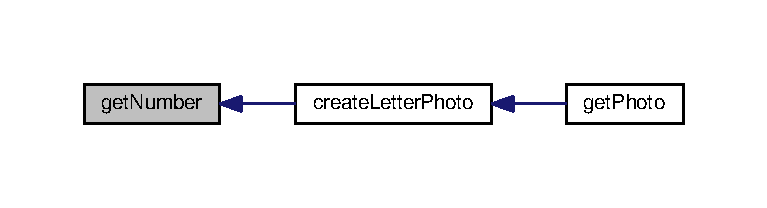
\includegraphics[width=350pt]{a00005_ae03bcf255a5fc2f7d29438a9a310144e_icgraph}
\end{center}
\end{figure}


\hypertarget{a00005_a589071d4450e576bcf705b147a5d8dfc}{\index{org\+::opensecurity\+::sms\+::model\+::\+Contact@{org\+::opensecurity\+::sms\+::model\+::\+Contact}!get\+Photo@{get\+Photo}}
\index{get\+Photo@{get\+Photo}!org\+::opensecurity\+::sms\+::model\+::\+Contact@{org\+::opensecurity\+::sms\+::model\+::\+Contact}}
\subsubsection[{get\+Photo}]{\setlength{\rightskip}{0pt plus 5cm}final Bitmap get\+Photo (
\begin{DoxyParamCaption}
\item[{Content\+Resolver}]{content\+Resolver}
\end{DoxyParamCaption}
)}}\label{a00005_a589071d4450e576bcf705b147a5d8dfc}
To get his photo 
\begin{DoxyParams}{Parameters}
{\em content\+Resolver} & to manage access to a structured set of data in your phone \\
\hline
\end{DoxyParams}
\begin{DoxyReturn}{Returns}
bitmap picture of our contact 
\end{DoxyReturn}


Here is the call graph for this function\+:
\nopagebreak
\begin{figure}[H]
\begin{center}
\leavevmode
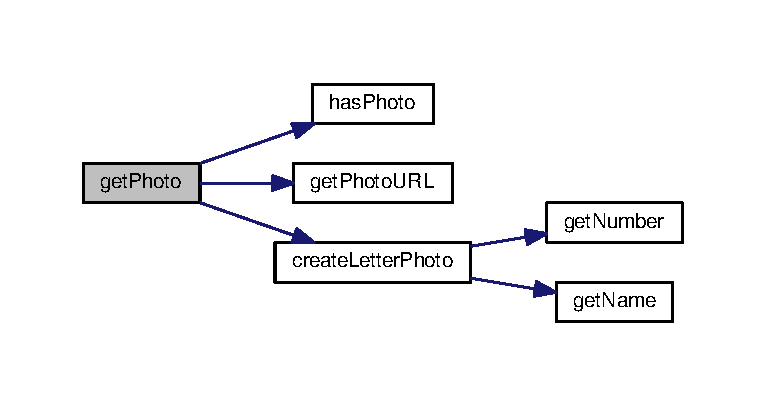
\includegraphics[width=350pt]{a00005_a589071d4450e576bcf705b147a5d8dfc_cgraph}
\end{center}
\end{figure}


\hypertarget{a00005_acb254f588afdb1371b7fcf708e8e665d}{\index{org\+::opensecurity\+::sms\+::model\+::\+Contact@{org\+::opensecurity\+::sms\+::model\+::\+Contact}!get\+Photo\+U\+R\+L@{get\+Photo\+U\+R\+L}}
\index{get\+Photo\+U\+R\+L@{get\+Photo\+U\+R\+L}!org\+::opensecurity\+::sms\+::model\+::\+Contact@{org\+::opensecurity\+::sms\+::model\+::\+Contact}}
\subsubsection[{get\+Photo\+U\+R\+L}]{\setlength{\rightskip}{0pt plus 5cm}String get\+Photo\+U\+R\+L (
\begin{DoxyParamCaption}
{}
\end{DoxyParamCaption}
)}}\label{a00005_acb254f588afdb1371b7fcf708e8e665d}
to get his photo\+Url (in database) \begin{DoxyReturn}{Returns}
the photo\+Url of current contact 
\end{DoxyReturn}


Here is the caller graph for this function\+:
\nopagebreak
\begin{figure}[H]
\begin{center}
\leavevmode
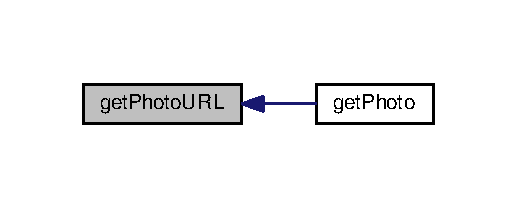
\includegraphics[width=248pt]{a00005_acb254f588afdb1371b7fcf708e8e665d_icgraph}
\end{center}
\end{figure}


\hypertarget{a00005_ad0e00784944089a9ece0934817c8976b}{\index{org\+::opensecurity\+::sms\+::model\+::\+Contact@{org\+::opensecurity\+::sms\+::model\+::\+Contact}!get\+Thread\+Id@{get\+Thread\+Id}}
\index{get\+Thread\+Id@{get\+Thread\+Id}!org\+::opensecurity\+::sms\+::model\+::\+Contact@{org\+::opensecurity\+::sms\+::model\+::\+Contact}}
\subsubsection[{get\+Thread\+Id}]{\setlength{\rightskip}{0pt plus 5cm}int get\+Thread\+Id (
\begin{DoxyParamCaption}
{}
\end{DoxyParamCaption}
)}}\label{a00005_ad0e00784944089a9ece0934817c8976b}
to get the primary key of current contact \begin{DoxyReturn}{Returns}
the thread\+Id of one contact 
\end{DoxyReturn}


Here is the caller graph for this function\+:
\nopagebreak
\begin{figure}[H]
\begin{center}
\leavevmode
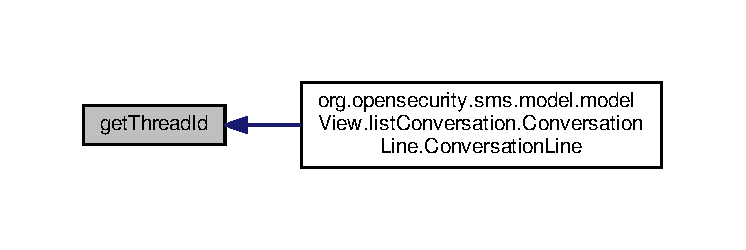
\includegraphics[width=350pt]{a00005_ad0e00784944089a9ece0934817c8976b_icgraph}
\end{center}
\end{figure}


\hypertarget{a00005_a6f861ae47c26fefab4e8e0cea9a1c979}{\index{org\+::opensecurity\+::sms\+::model\+::\+Contact@{org\+::opensecurity\+::sms\+::model\+::\+Contact}!has\+Photo@{has\+Photo}}
\index{has\+Photo@{has\+Photo}!org\+::opensecurity\+::sms\+::model\+::\+Contact@{org\+::opensecurity\+::sms\+::model\+::\+Contact}}
\subsubsection[{has\+Photo}]{\setlength{\rightskip}{0pt plus 5cm}boolean has\+Photo (
\begin{DoxyParamCaption}
{}
\end{DoxyParamCaption}
)}}\label{a00005_a6f861ae47c26fefab4e8e0cea9a1c979}
to know if a contact has a picture \begin{DoxyReturn}{Returns}
true if contact has a picture in database 
\end{DoxyReturn}


Here is the caller graph for this function\+:
\nopagebreak
\begin{figure}[H]
\begin{center}
\leavevmode
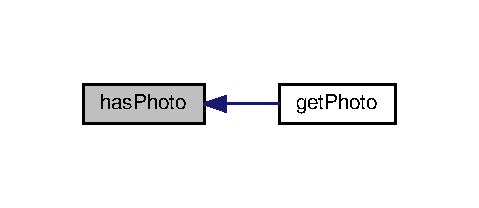
\includegraphics[width=230pt]{a00005_a6f861ae47c26fefab4e8e0cea9a1c979_icgraph}
\end{center}
\end{figure}


\hypertarget{a00005_ad737b36b74be994e0d8420797ed72f78}{\index{org\+::opensecurity\+::sms\+::model\+::\+Contact@{org\+::opensecurity\+::sms\+::model\+::\+Contact}!set\+Name@{set\+Name}}
\index{set\+Name@{set\+Name}!org\+::opensecurity\+::sms\+::model\+::\+Contact@{org\+::opensecurity\+::sms\+::model\+::\+Contact}}
\subsubsection[{set\+Name}]{\setlength{\rightskip}{0pt plus 5cm}void set\+Name (
\begin{DoxyParamCaption}
\item[{String}]{name}
\end{DoxyParamCaption}
)}}\label{a00005_ad737b36b74be994e0d8420797ed72f78}
to set the name of a current contact 
\begin{DoxyParams}{Parameters}
{\em name} & his name \\
\hline
\end{DoxyParams}


Here is the caller graph for this function\+:
\nopagebreak
\begin{figure}[H]
\begin{center}
\leavevmode
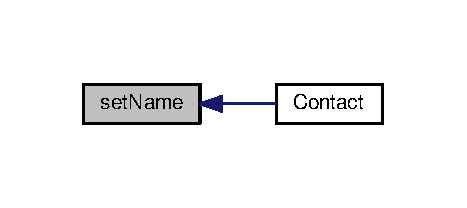
\includegraphics[width=224pt]{a00005_ad737b36b74be994e0d8420797ed72f78_icgraph}
\end{center}
\end{figure}


\hypertarget{a00005_a5bad44419074a927bf68c94245f36890}{\index{org\+::opensecurity\+::sms\+::model\+::\+Contact@{org\+::opensecurity\+::sms\+::model\+::\+Contact}!set\+Nb\+Messages@{set\+Nb\+Messages}}
\index{set\+Nb\+Messages@{set\+Nb\+Messages}!org\+::opensecurity\+::sms\+::model\+::\+Contact@{org\+::opensecurity\+::sms\+::model\+::\+Contact}}
\subsubsection[{set\+Nb\+Messages}]{\setlength{\rightskip}{0pt plus 5cm}void set\+Nb\+Messages (
\begin{DoxyParamCaption}
\item[{int}]{nb\+Messages}
\end{DoxyParamCaption}
)}}\label{a00005_a5bad44419074a927bf68c94245f36890}
to set the number of messages between us and our contact 
\begin{DoxyParams}{Parameters}
{\em nb\+Messages} & the number of messages between us and our contact \\
\hline
\end{DoxyParams}


Here is the caller graph for this function\+:
\nopagebreak
\begin{figure}[H]
\begin{center}
\leavevmode
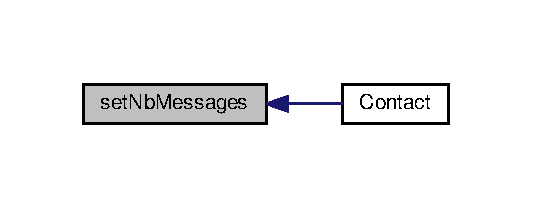
\includegraphics[width=256pt]{a00005_a5bad44419074a927bf68c94245f36890_icgraph}
\end{center}
\end{figure}


\hypertarget{a00005_a5248a434af8755dc41918e83e8cbe2cc}{\index{org\+::opensecurity\+::sms\+::model\+::\+Contact@{org\+::opensecurity\+::sms\+::model\+::\+Contact}!set\+Number@{set\+Number}}
\index{set\+Number@{set\+Number}!org\+::opensecurity\+::sms\+::model\+::\+Contact@{org\+::opensecurity\+::sms\+::model\+::\+Contact}}
\subsubsection[{set\+Number}]{\setlength{\rightskip}{0pt plus 5cm}void set\+Number (
\begin{DoxyParamCaption}
\item[{String}]{number}
\end{DoxyParamCaption}
)}}\label{a00005_a5248a434af8755dc41918e83e8cbe2cc}
to set the phone\+Number of our contact 
\begin{DoxyParams}{Parameters}
{\em number} & the phone\+Number in database \\
\hline
\end{DoxyParams}


Here is the caller graph for this function\+:
\nopagebreak
\begin{figure}[H]
\begin{center}
\leavevmode
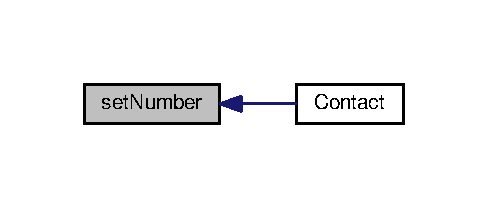
\includegraphics[width=234pt]{a00005_a5248a434af8755dc41918e83e8cbe2cc_icgraph}
\end{center}
\end{figure}


\hypertarget{a00005_a26188abec636b2754749851d108157c9}{\index{org\+::opensecurity\+::sms\+::model\+::\+Contact@{org\+::opensecurity\+::sms\+::model\+::\+Contact}!set\+Photo\+U\+R\+L@{set\+Photo\+U\+R\+L}}
\index{set\+Photo\+U\+R\+L@{set\+Photo\+U\+R\+L}!org\+::opensecurity\+::sms\+::model\+::\+Contact@{org\+::opensecurity\+::sms\+::model\+::\+Contact}}
\subsubsection[{set\+Photo\+U\+R\+L}]{\setlength{\rightskip}{0pt plus 5cm}void set\+Photo\+U\+R\+L (
\begin{DoxyParamCaption}
\item[{String}]{photo\+U\+R\+L}
\end{DoxyParamCaption}
)}}\label{a00005_a26188abec636b2754749851d108157c9}
to set his photo\+Url (in database) 
\begin{DoxyParams}{Parameters}
{\em photo\+U\+R\+L} & photo\+Url of current contact \\
\hline
\end{DoxyParams}


Here is the caller graph for this function\+:
\nopagebreak
\begin{figure}[H]
\begin{center}
\leavevmode
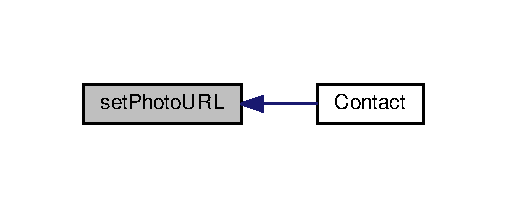
\includegraphics[width=244pt]{a00005_a26188abec636b2754749851d108157c9_icgraph}
\end{center}
\end{figure}


\hypertarget{a00005_a0d24ce5a0d8f054366321a58db5d4d0a}{\index{org\+::opensecurity\+::sms\+::model\+::\+Contact@{org\+::opensecurity\+::sms\+::model\+::\+Contact}!set\+Thread\+Id@{set\+Thread\+Id}}
\index{set\+Thread\+Id@{set\+Thread\+Id}!org\+::opensecurity\+::sms\+::model\+::\+Contact@{org\+::opensecurity\+::sms\+::model\+::\+Contact}}
\subsubsection[{set\+Thread\+Id}]{\setlength{\rightskip}{0pt plus 5cm}void set\+Thread\+Id (
\begin{DoxyParamCaption}
\item[{int}]{thread\+Id}
\end{DoxyParamCaption}
)}}\label{a00005_a0d24ce5a0d8f054366321a58db5d4d0a}
to set the thread\+Id of one contact 
\begin{DoxyParams}{Parameters}
{\em thread\+Id} & the thread\+Id for the current contact \\
\hline
\end{DoxyParams}


Here is the caller graph for this function\+:
\nopagebreak
\begin{figure}[H]
\begin{center}
\leavevmode
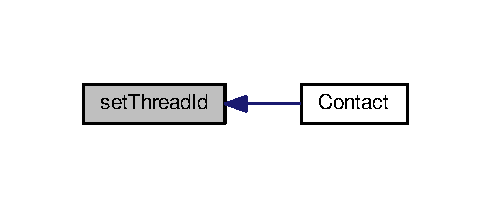
\includegraphics[width=236pt]{a00005_a0d24ce5a0d8f054366321a58db5d4d0a_icgraph}
\end{center}
\end{figure}




\subsection{Member Data Documentation}
\hypertarget{a00005_a9a2326f35466e54c36c070829245c557}{\index{org\+::opensecurity\+::sms\+::model\+::\+Contact@{org\+::opensecurity\+::sms\+::model\+::\+Contact}!name@{name}}
\index{name@{name}!org\+::opensecurity\+::sms\+::model\+::\+Contact@{org\+::opensecurity\+::sms\+::model\+::\+Contact}}
\subsubsection[{name}]{\setlength{\rightskip}{0pt plus 5cm}String name\hspace{0.3cm}{\ttfamily [private]}}}\label{a00005_a9a2326f35466e54c36c070829245c557}
name is the name of contact, number is his phone\+Number and photo\+Url is his picture contact \hypertarget{a00005_a88c965ed9f3385173d81f6bd02caac09}{\index{org\+::opensecurity\+::sms\+::model\+::\+Contact@{org\+::opensecurity\+::sms\+::model\+::\+Contact}!nb\+Messages@{nb\+Messages}}
\index{nb\+Messages@{nb\+Messages}!org\+::opensecurity\+::sms\+::model\+::\+Contact@{org\+::opensecurity\+::sms\+::model\+::\+Contact}}
\subsubsection[{nb\+Messages}]{\setlength{\rightskip}{0pt plus 5cm}int nb\+Messages\hspace{0.3cm}{\ttfamily [package]}}}\label{a00005_a88c965ed9f3385173d81f6bd02caac09}
\hypertarget{a00005_a59be7928addfd6c2307fa665d9d0eb3a}{\index{org\+::opensecurity\+::sms\+::model\+::\+Contact@{org\+::opensecurity\+::sms\+::model\+::\+Contact}!number@{number}}
\index{number@{number}!org\+::opensecurity\+::sms\+::model\+::\+Contact@{org\+::opensecurity\+::sms\+::model\+::\+Contact}}
\subsubsection[{number}]{\setlength{\rightskip}{0pt plus 5cm}String number\hspace{0.3cm}{\ttfamily [package]}}}\label{a00005_a59be7928addfd6c2307fa665d9d0eb3a}
\hypertarget{a00005_a6300d0c52298ebf7049df45c04ca1879}{\index{org\+::opensecurity\+::sms\+::model\+::\+Contact@{org\+::opensecurity\+::sms\+::model\+::\+Contact}!photo\+U\+R\+L@{photo\+U\+R\+L}}
\index{photo\+U\+R\+L@{photo\+U\+R\+L}!org\+::opensecurity\+::sms\+::model\+::\+Contact@{org\+::opensecurity\+::sms\+::model\+::\+Contact}}
\subsubsection[{photo\+U\+R\+L}]{\setlength{\rightskip}{0pt plus 5cm}String photo\+U\+R\+L\hspace{0.3cm}{\ttfamily [package]}}}\label{a00005_a6300d0c52298ebf7049df45c04ca1879}
\hypertarget{a00005_afdf9018750ccb340d2173b2a3da1e755}{\index{org\+::opensecurity\+::sms\+::model\+::\+Contact@{org\+::opensecurity\+::sms\+::model\+::\+Contact}!thread\+Id@{thread\+Id}}
\index{thread\+Id@{thread\+Id}!org\+::opensecurity\+::sms\+::model\+::\+Contact@{org\+::opensecurity\+::sms\+::model\+::\+Contact}}
\subsubsection[{thread\+Id}]{\setlength{\rightskip}{0pt plus 5cm}int thread\+Id\hspace{0.3cm}{\ttfamily [private]}}}\label{a00005_afdf9018750ccb340d2173b2a3da1e755}
thread\+Id is like a primary key for on contact in database 

The documentation for this class was generated from the following file\+:\begin{DoxyCompactItemize}
\item 
app/src/main/java/org/opensecurity/sms/model/\hyperlink{a00017}{Contact.\+java}\end{DoxyCompactItemize}

\hypertarget{a00006}{\section{Conversation\+Activity Class Reference}
\label{a00006}\index{Conversation\+Activity@{Conversation\+Activity}}
}


Inheritance diagram for Conversation\+Activity\+:
\nopagebreak
\begin{figure}[H]
\begin{center}
\leavevmode
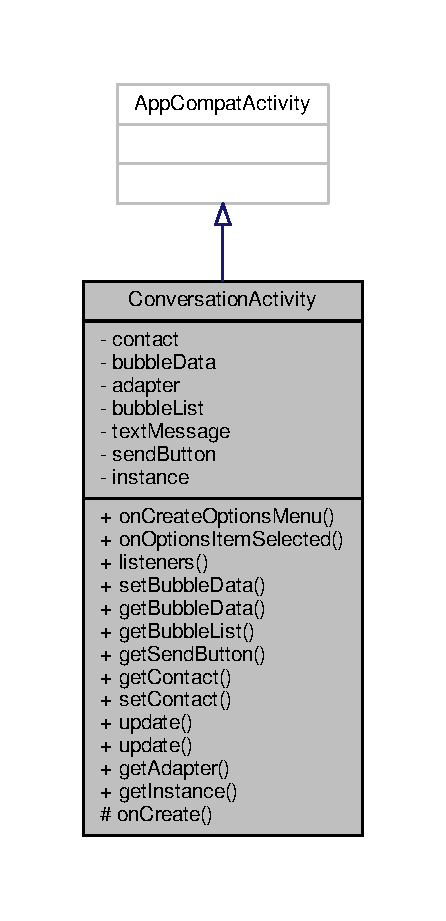
\includegraphics[width=214pt]{a00078}
\end{center}
\end{figure}


Collaboration diagram for Conversation\+Activity\+:
\nopagebreak
\begin{figure}[H]
\begin{center}
\leavevmode
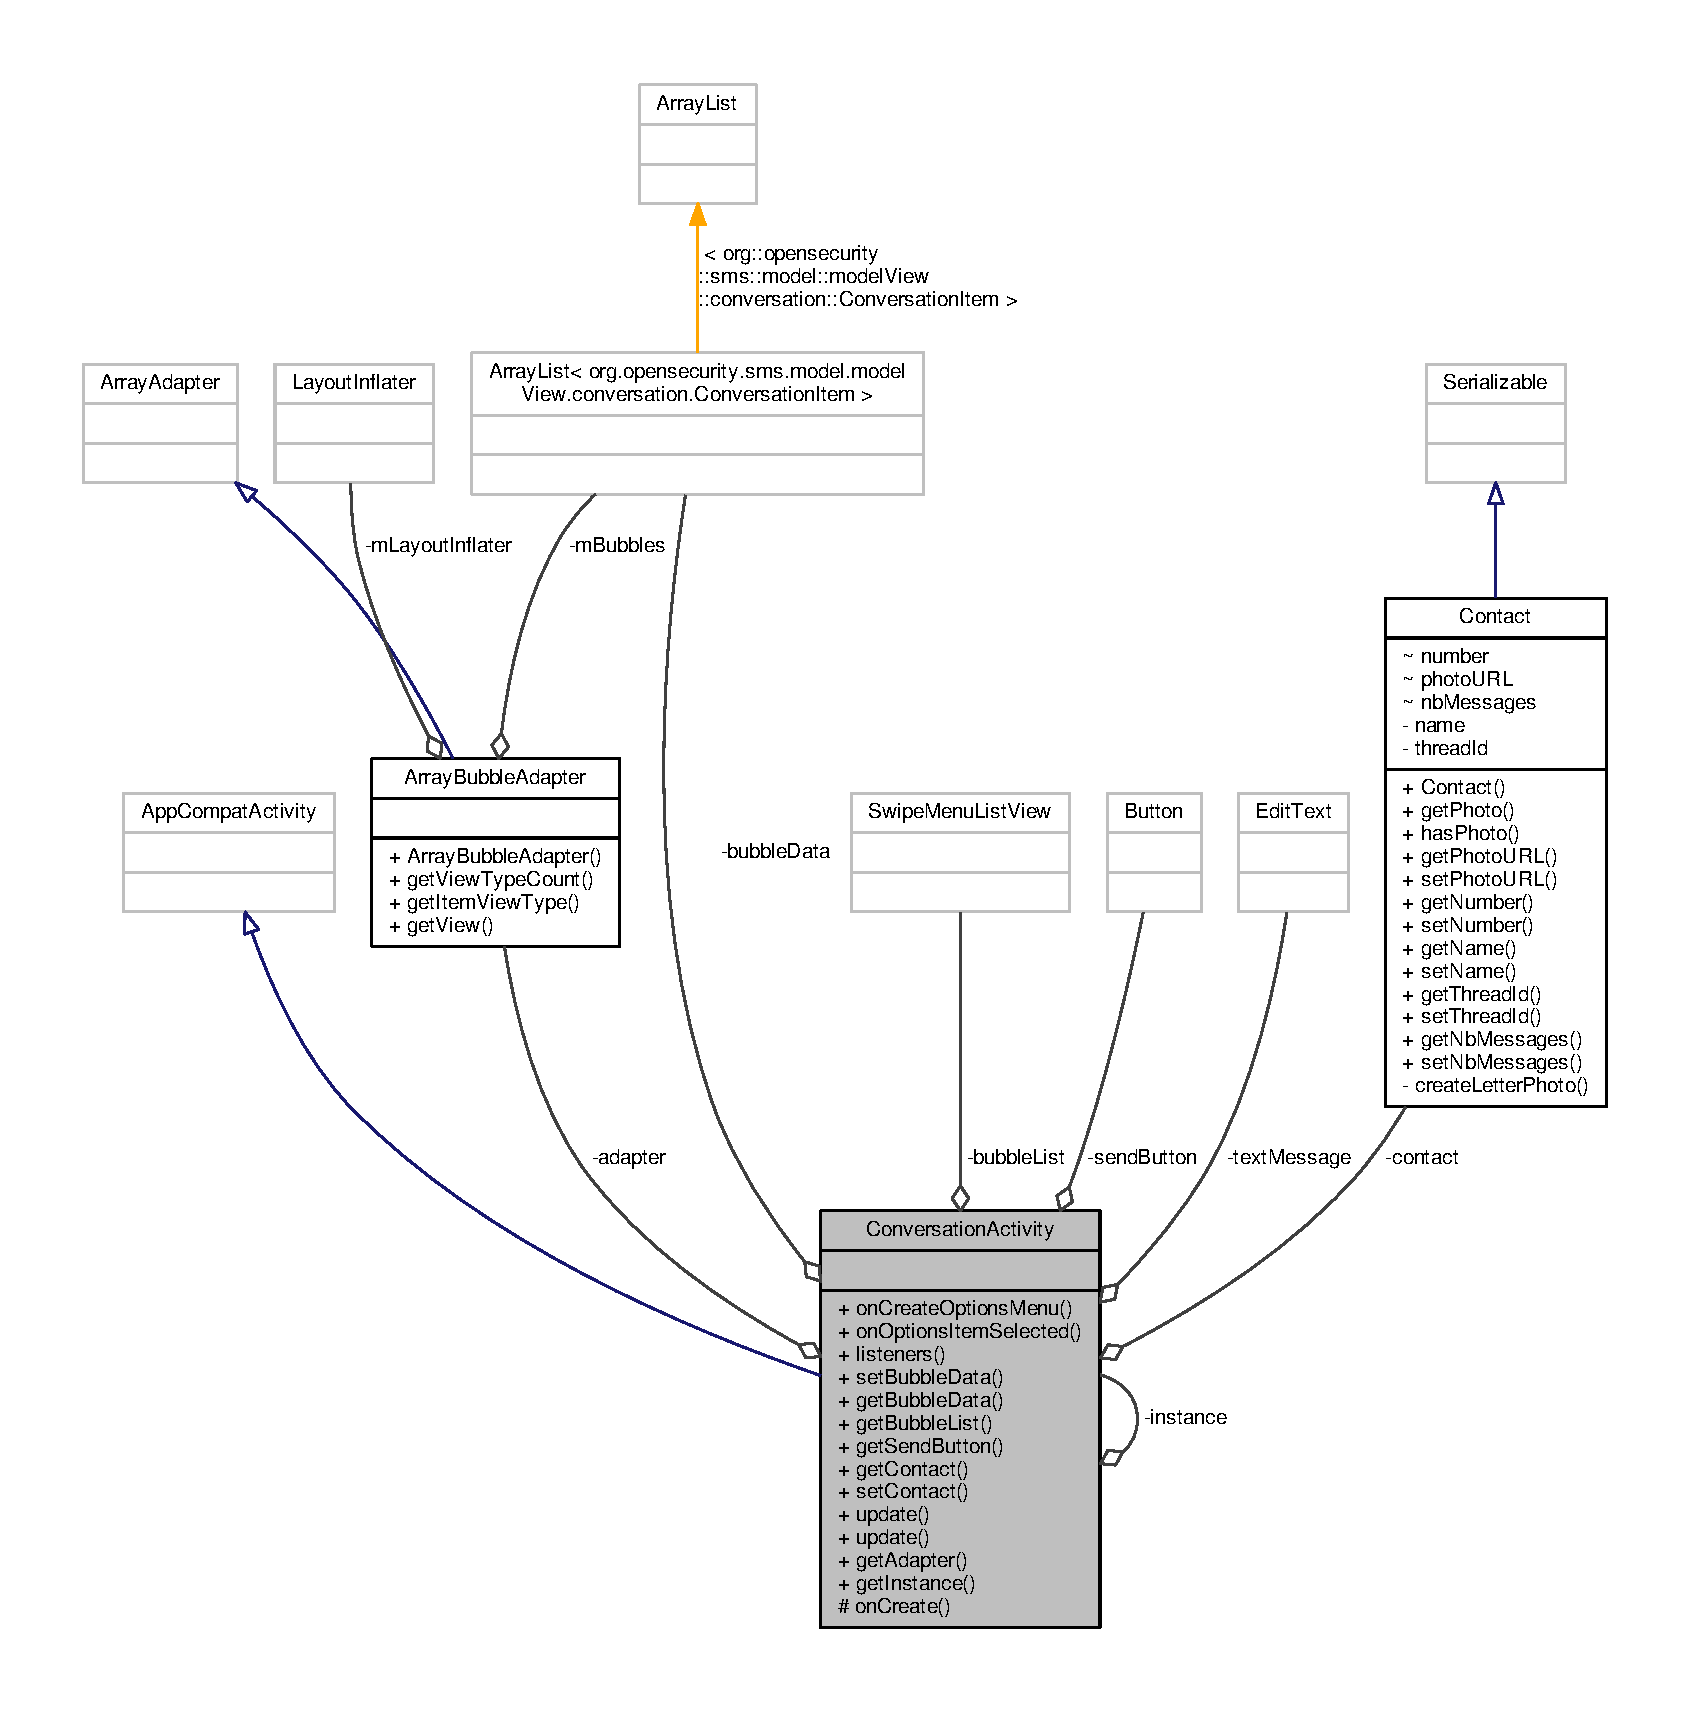
\includegraphics[width=350pt]{a00079}
\end{center}
\end{figure}
\subsection*{Public Member Functions}
\begin{DoxyCompactItemize}
\item 
boolean \hyperlink{a00006_a8f7d87763ddaf085205a54e8477ecfce}{on\+Create\+Options\+Menu} (Menu menu)
\item 
boolean \hyperlink{a00006_a37a55c533c74b60c0290ef1329d74e65}{on\+Options\+Item\+Selected} (Menu\+Item item)
\item 
void \hyperlink{a00006_a92b8e0730130e1184a8cdbd89590779d}{listeners} ()
\item 
void \hyperlink{a00006_a1e3fee8580ec4092ffc6e3ce9d44f2b9}{set\+Bubble\+Data} (Array\+List$<$ \hyperlink{a00007}{Conversation\+Item} $>$ \hyperlink{a00006_a68544a0bda28776dfb51718a3c71bf69}{bubble\+Data})
\item 
Array\+List$<$ \hyperlink{a00007}{Conversation\+Item} $>$ \hyperlink{a00006_ac8e14177e6079becbb8bc1f8b35197e0}{get\+Bubble\+Data} ()
\item 
Swipe\+Menu\+List\+View \hyperlink{a00006_af293d3ea5f145650e06a96d2bae482da}{get\+Bubble\+List} ()
\item 
Button \hyperlink{a00006_a57576f3fc93bfa5a685ed5ee30fe113c}{get\+Send\+Button} ()
\item 
\hyperlink{a00005}{Contact} \hyperlink{a00006_adb647c7ae09f1d5755db63d701968925}{get\+Contact} ()
\item 
void \hyperlink{a00006_abef3c7b6635dc06ac6b8e4b37c51b37f}{set\+Contact} (\hyperlink{a00005}{Contact} \hyperlink{a00006_a3459849ab29ad684658dbcd0cf8c5d5a}{contact})
\item 
void \hyperlink{a00006_aa2825578f585a8a32958eaf0ce8df7b8}{update} (Intent intent)
\item 
void \hyperlink{a00006_ac5c54df7ed3b930268c8d7752c101725}{update} ()
\item 
\hyperlink{a00002}{Array\+Bubble\+Adapter} \hyperlink{a00006_a06738816ea7799569af8fa119bb49f7e}{get\+Adapter} ()
\end{DoxyCompactItemize}
\subsection*{Static Public Member Functions}
\begin{DoxyCompactItemize}
\item 
static \hyperlink{a00006}{Conversation\+Activity} \hyperlink{a00006_a7ebafa56e442a2f16c4afe044e65695b}{get\+Instance} ()
\end{DoxyCompactItemize}
\subsection*{Protected Member Functions}
\begin{DoxyCompactItemize}
\item 
void \hyperlink{a00006_a85e87cb5ced88dff7c8173ecc4f636d1}{on\+Create} (Bundle saved\+Instance\+State)
\end{DoxyCompactItemize}
\subsection*{Private Attributes}
\begin{DoxyCompactItemize}
\item 
\hyperlink{a00005}{Contact} \hyperlink{a00006_a3459849ab29ad684658dbcd0cf8c5d5a}{contact}
\item 
Array\+List$<$ \hyperlink{a00007}{Conversation\+Item} $>$ \hyperlink{a00006_a68544a0bda28776dfb51718a3c71bf69}{bubble\+Data}
\item 
\hyperlink{a00002}{Array\+Bubble\+Adapter} \hyperlink{a00006_adaad4a865e59995c45ef2ad13f6e88a9}{adapter}
\item 
Swipe\+Menu\+List\+View \hyperlink{a00006_ae5bb074a89738fa417e643960b0041c6}{bubble\+List}
\item 
Edit\+Text \hyperlink{a00006_abc418be8d11246756bfcb7f95123a88d}{text\+Message}
\item 
Button \hyperlink{a00006_a2e4d147a434708e05027f41ecf9ed577}{send\+Button}
\end{DoxyCompactItemize}
\subsection*{Static Private Attributes}
\begin{DoxyCompactItemize}
\item 
static \hyperlink{a00006}{Conversation\+Activity} \hyperlink{a00006_a64a39fb2b7f756356462736dfbdb9f9f}{instance}
\end{DoxyCompactItemize}


\subsection{Detailed Description}
This class is an activity for displaying one conversation bitween us and another contact. 

\subsection{Member Function Documentation}
\hypertarget{a00006_a06738816ea7799569af8fa119bb49f7e}{\index{org\+::opensecurity\+::sms\+::view\+::\+Conversation\+Activity@{org\+::opensecurity\+::sms\+::view\+::\+Conversation\+Activity}!get\+Adapter@{get\+Adapter}}
\index{get\+Adapter@{get\+Adapter}!org\+::opensecurity\+::sms\+::view\+::\+Conversation\+Activity@{org\+::opensecurity\+::sms\+::view\+::\+Conversation\+Activity}}
\subsubsection[{get\+Adapter}]{\setlength{\rightskip}{0pt plus 5cm}{\bf Array\+Bubble\+Adapter} get\+Adapter (
\begin{DoxyParamCaption}
{}
\end{DoxyParamCaption}
)}}\label{a00006_a06738816ea7799569af8fa119bb49f7e}
To get the adapter (design) \begin{DoxyReturn}{Returns}
the adapter of current activity 
\end{DoxyReturn}


Here is the caller graph for this function\+:
\nopagebreak
\begin{figure}[H]
\begin{center}
\leavevmode
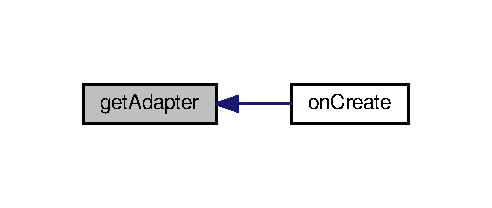
\includegraphics[width=236pt]{a00006_a06738816ea7799569af8fa119bb49f7e_icgraph}
\end{center}
\end{figure}


\hypertarget{a00006_ac8e14177e6079becbb8bc1f8b35197e0}{\index{org\+::opensecurity\+::sms\+::view\+::\+Conversation\+Activity@{org\+::opensecurity\+::sms\+::view\+::\+Conversation\+Activity}!get\+Bubble\+Data@{get\+Bubble\+Data}}
\index{get\+Bubble\+Data@{get\+Bubble\+Data}!org\+::opensecurity\+::sms\+::view\+::\+Conversation\+Activity@{org\+::opensecurity\+::sms\+::view\+::\+Conversation\+Activity}}
\subsubsection[{get\+Bubble\+Data}]{\setlength{\rightskip}{0pt plus 5cm}Array\+List$<${\bf Conversation\+Item}$>$ get\+Bubble\+Data (
\begin{DoxyParamCaption}
{}
\end{DoxyParamCaption}
)}}\label{a00006_ac8e14177e6079becbb8bc1f8b35197e0}
Just return the bubble\+Data which are loaded in the activity \begin{DoxyReturn}{Returns}
bubble\+Data of current activity 
\end{DoxyReturn}


Here is the caller graph for this function\+:
\nopagebreak
\begin{figure}[H]
\begin{center}
\leavevmode
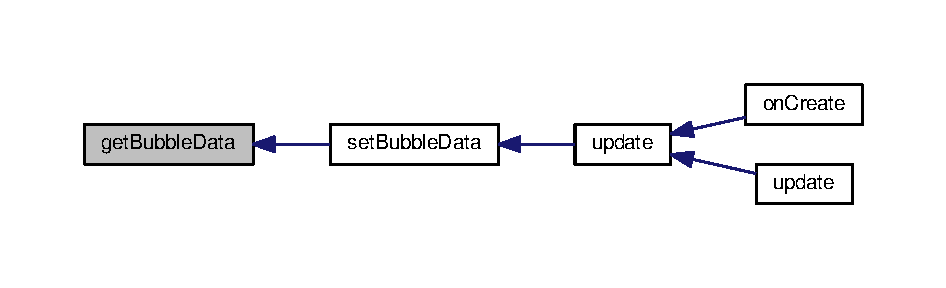
\includegraphics[width=350pt]{a00006_ac8e14177e6079becbb8bc1f8b35197e0_icgraph}
\end{center}
\end{figure}


\hypertarget{a00006_af293d3ea5f145650e06a96d2bae482da}{\index{org\+::opensecurity\+::sms\+::view\+::\+Conversation\+Activity@{org\+::opensecurity\+::sms\+::view\+::\+Conversation\+Activity}!get\+Bubble\+List@{get\+Bubble\+List}}
\index{get\+Bubble\+List@{get\+Bubble\+List}!org\+::opensecurity\+::sms\+::view\+::\+Conversation\+Activity@{org\+::opensecurity\+::sms\+::view\+::\+Conversation\+Activity}}
\subsubsection[{get\+Bubble\+List}]{\setlength{\rightskip}{0pt plus 5cm}Swipe\+Menu\+List\+View get\+Bubble\+List (
\begin{DoxyParamCaption}
{}
\end{DoxyParamCaption}
)}}\label{a00006_af293d3ea5f145650e06a96d2bae482da}
To return the menu\+List\+View of bubbles. \begin{DoxyReturn}{Returns}
the List\+View of current activity 
\end{DoxyReturn}


Here is the caller graph for this function\+:
\nopagebreak
\begin{figure}[H]
\begin{center}
\leavevmode
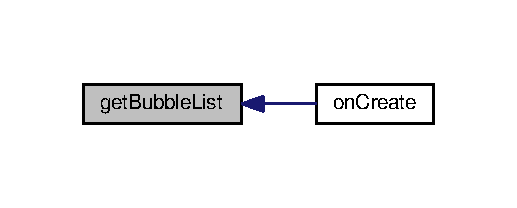
\includegraphics[width=248pt]{a00006_af293d3ea5f145650e06a96d2bae482da_icgraph}
\end{center}
\end{figure}


\hypertarget{a00006_adb647c7ae09f1d5755db63d701968925}{\index{org\+::opensecurity\+::sms\+::view\+::\+Conversation\+Activity@{org\+::opensecurity\+::sms\+::view\+::\+Conversation\+Activity}!get\+Contact@{get\+Contact}}
\index{get\+Contact@{get\+Contact}!org\+::opensecurity\+::sms\+::view\+::\+Conversation\+Activity@{org\+::opensecurity\+::sms\+::view\+::\+Conversation\+Activity}}
\subsubsection[{get\+Contact}]{\setlength{\rightskip}{0pt plus 5cm}{\bf Contact} get\+Contact (
\begin{DoxyParamCaption}
{}
\end{DoxyParamCaption}
)}}\label{a00006_adb647c7ae09f1d5755db63d701968925}
To get the contact of our current activity. \begin{DoxyReturn}{Returns}
the current contact of selected activity conversation 
\end{DoxyReturn}


Here is the caller graph for this function\+:
\nopagebreak
\begin{figure}[H]
\begin{center}
\leavevmode
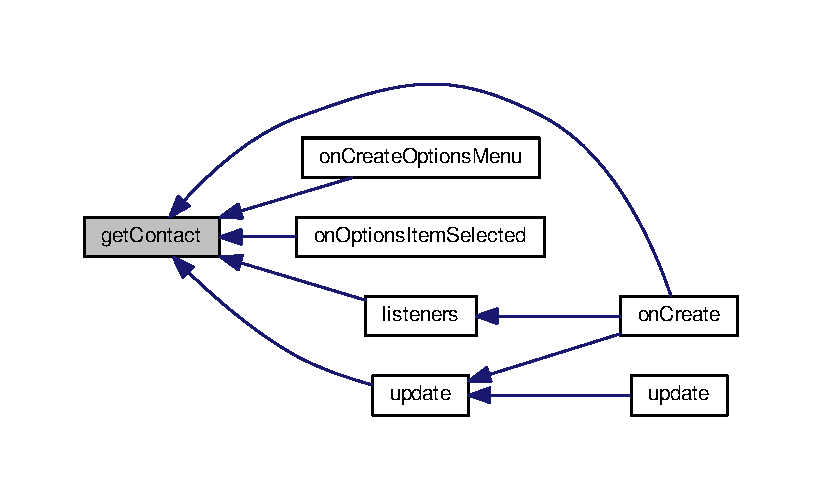
\includegraphics[width=350pt]{a00006_adb647c7ae09f1d5755db63d701968925_icgraph}
\end{center}
\end{figure}


\hypertarget{a00006_a7ebafa56e442a2f16c4afe044e65695b}{\index{org\+::opensecurity\+::sms\+::view\+::\+Conversation\+Activity@{org\+::opensecurity\+::sms\+::view\+::\+Conversation\+Activity}!get\+Instance@{get\+Instance}}
\index{get\+Instance@{get\+Instance}!org\+::opensecurity\+::sms\+::view\+::\+Conversation\+Activity@{org\+::opensecurity\+::sms\+::view\+::\+Conversation\+Activity}}
\subsubsection[{get\+Instance}]{\setlength{\rightskip}{0pt plus 5cm}static {\bf Conversation\+Activity} get\+Instance (
\begin{DoxyParamCaption}
{}
\end{DoxyParamCaption}
)\hspace{0.3cm}{\ttfamily [static]}}}\label{a00006_a7ebafa56e442a2f16c4afe044e65695b}
To return the current instance. Be sure that is the only one instance (singleton pattern) \begin{DoxyReturn}{Returns}
the instance of current activity (=this) 
\end{DoxyReturn}


Here is the caller graph for this function\+:
\nopagebreak
\begin{figure}[H]
\begin{center}
\leavevmode
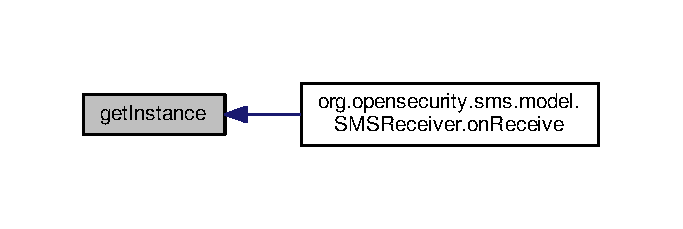
\includegraphics[width=328pt]{a00006_a7ebafa56e442a2f16c4afe044e65695b_icgraph}
\end{center}
\end{figure}


\hypertarget{a00006_a57576f3fc93bfa5a685ed5ee30fe113c}{\index{org\+::opensecurity\+::sms\+::view\+::\+Conversation\+Activity@{org\+::opensecurity\+::sms\+::view\+::\+Conversation\+Activity}!get\+Send\+Button@{get\+Send\+Button}}
\index{get\+Send\+Button@{get\+Send\+Button}!org\+::opensecurity\+::sms\+::view\+::\+Conversation\+Activity@{org\+::opensecurity\+::sms\+::view\+::\+Conversation\+Activity}}
\subsubsection[{get\+Send\+Button}]{\setlength{\rightskip}{0pt plus 5cm}Button get\+Send\+Button (
\begin{DoxyParamCaption}
{}
\end{DoxyParamCaption}
)}}\label{a00006_a57576f3fc93bfa5a685ed5ee30fe113c}
To return the send\+Button of this activity. \begin{DoxyReturn}{Returns}
the Button to send messages in this activity 
\end{DoxyReturn}


Here is the caller graph for this function\+:
\nopagebreak
\begin{figure}[H]
\begin{center}
\leavevmode
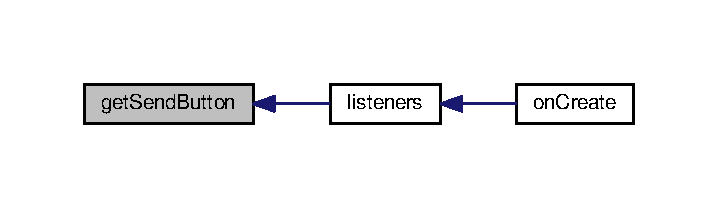
\includegraphics[width=344pt]{a00006_a57576f3fc93bfa5a685ed5ee30fe113c_icgraph}
\end{center}
\end{figure}


\hypertarget{a00006_a92b8e0730130e1184a8cdbd89590779d}{\index{org\+::opensecurity\+::sms\+::view\+::\+Conversation\+Activity@{org\+::opensecurity\+::sms\+::view\+::\+Conversation\+Activity}!listeners@{listeners}}
\index{listeners@{listeners}!org\+::opensecurity\+::sms\+::view\+::\+Conversation\+Activity@{org\+::opensecurity\+::sms\+::view\+::\+Conversation\+Activity}}
\subsubsection[{listeners}]{\setlength{\rightskip}{0pt plus 5cm}void listeners (
\begin{DoxyParamCaption}
{}
\end{DoxyParamCaption}
)}}\label{a00006_a92b8e0730130e1184a8cdbd89590779d}
contains listeners of the activity First listener. We call send\+S\+M\+S function and after that, if the sms exists, we create a new bubble and we reload the Adapter.

Here is the call graph for this function\+:
\nopagebreak
\begin{figure}[H]
\begin{center}
\leavevmode
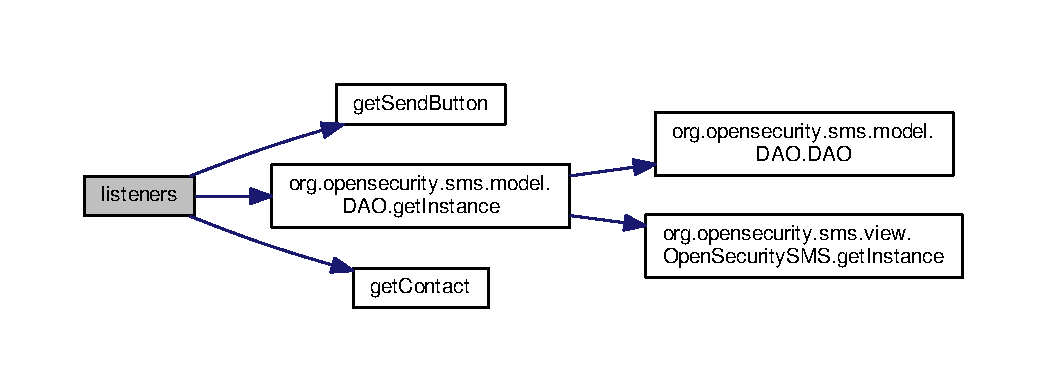
\includegraphics[width=350pt]{a00006_a92b8e0730130e1184a8cdbd89590779d_cgraph}
\end{center}
\end{figure}




Here is the caller graph for this function\+:
\nopagebreak
\begin{figure}[H]
\begin{center}
\leavevmode
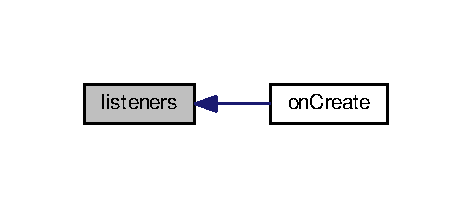
\includegraphics[width=226pt]{a00006_a92b8e0730130e1184a8cdbd89590779d_icgraph}
\end{center}
\end{figure}


\hypertarget{a00006_a85e87cb5ced88dff7c8173ecc4f636d1}{\index{org\+::opensecurity\+::sms\+::view\+::\+Conversation\+Activity@{org\+::opensecurity\+::sms\+::view\+::\+Conversation\+Activity}!on\+Create@{on\+Create}}
\index{on\+Create@{on\+Create}!org\+::opensecurity\+::sms\+::view\+::\+Conversation\+Activity@{org\+::opensecurity\+::sms\+::view\+::\+Conversation\+Activity}}
\subsubsection[{on\+Create}]{\setlength{\rightskip}{0pt plus 5cm}void on\+Create (
\begin{DoxyParamCaption}
\item[{Bundle}]{saved\+Instance\+State}
\end{DoxyParamCaption}
)\hspace{0.3cm}{\ttfamily [protected]}}}\label{a00006_a85e87cb5ced88dff7c8173ecc4f636d1}
To create the activity


\begin{DoxyParams}{Parameters}
{\em saved\+Instance\+State} & save the instance state to keep informations. \\
\hline
\end{DoxyParams}


Here is the call graph for this function\+:
\nopagebreak
\begin{figure}[H]
\begin{center}
\leavevmode
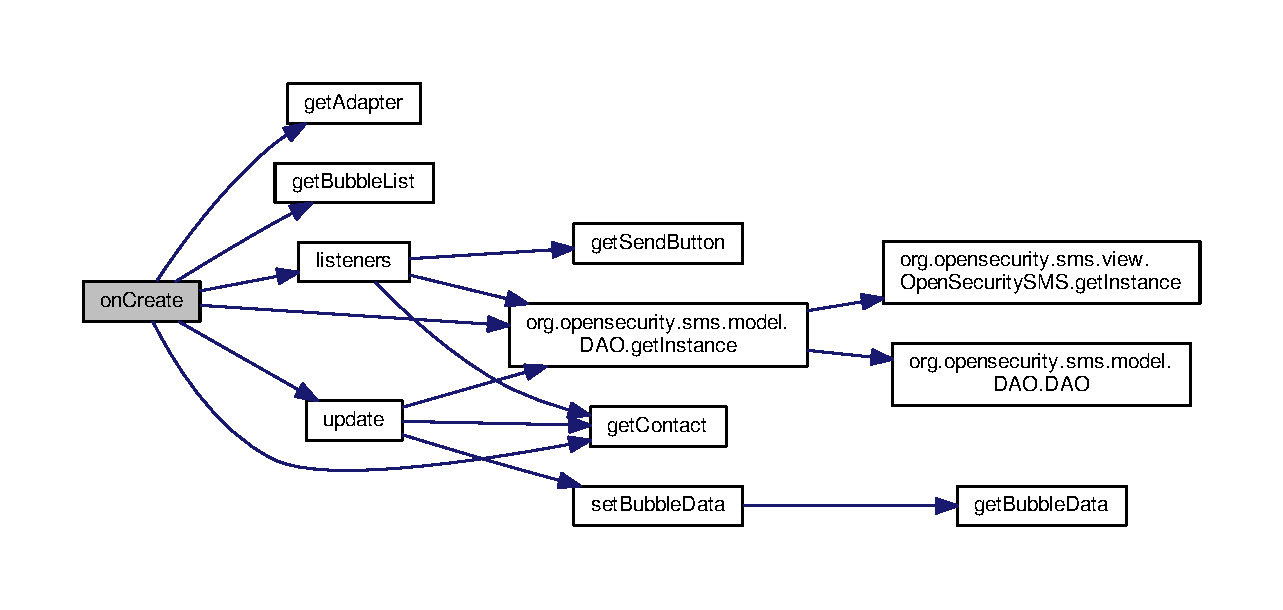
\includegraphics[width=350pt]{a00006_a85e87cb5ced88dff7c8173ecc4f636d1_cgraph}
\end{center}
\end{figure}


\hypertarget{a00006_a8f7d87763ddaf085205a54e8477ecfce}{\index{org\+::opensecurity\+::sms\+::view\+::\+Conversation\+Activity@{org\+::opensecurity\+::sms\+::view\+::\+Conversation\+Activity}!on\+Create\+Options\+Menu@{on\+Create\+Options\+Menu}}
\index{on\+Create\+Options\+Menu@{on\+Create\+Options\+Menu}!org\+::opensecurity\+::sms\+::view\+::\+Conversation\+Activity@{org\+::opensecurity\+::sms\+::view\+::\+Conversation\+Activity}}
\subsubsection[{on\+Create\+Options\+Menu}]{\setlength{\rightskip}{0pt plus 5cm}boolean on\+Create\+Options\+Menu (
\begin{DoxyParamCaption}
\item[{Menu}]{menu}
\end{DoxyParamCaption}
)}}\label{a00006_a8f7d87763ddaf085205a54e8477ecfce}
Use to create an option\+Menu.


\begin{DoxyParams}{Parameters}
{\em menu} & keep informations relative to the menu \\
\hline
\end{DoxyParams}
\begin{DoxyReturn}{Returns}
boolean if the menu is create or no 
\end{DoxyReturn}


Here is the call graph for this function\+:
\nopagebreak
\begin{figure}[H]
\begin{center}
\leavevmode
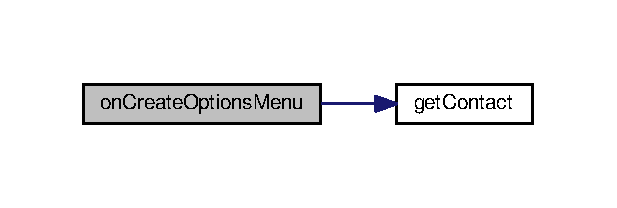
\includegraphics[width=296pt]{a00006_a8f7d87763ddaf085205a54e8477ecfce_cgraph}
\end{center}
\end{figure}


\hypertarget{a00006_a37a55c533c74b60c0290ef1329d74e65}{\index{org\+::opensecurity\+::sms\+::view\+::\+Conversation\+Activity@{org\+::opensecurity\+::sms\+::view\+::\+Conversation\+Activity}!on\+Options\+Item\+Selected@{on\+Options\+Item\+Selected}}
\index{on\+Options\+Item\+Selected@{on\+Options\+Item\+Selected}!org\+::opensecurity\+::sms\+::view\+::\+Conversation\+Activity@{org\+::opensecurity\+::sms\+::view\+::\+Conversation\+Activity}}
\subsubsection[{on\+Options\+Item\+Selected}]{\setlength{\rightskip}{0pt plus 5cm}boolean on\+Options\+Item\+Selected (
\begin{DoxyParamCaption}
\item[{Menu\+Item}]{item}
\end{DoxyParamCaption}
)}}\label{a00006_a37a55c533c74b60c0290ef1329d74e65}
To react when we select on item on the menu. 
\begin{DoxyParams}{Parameters}
{\em item} & the current selected item. \\
\hline
\end{DoxyParams}
\begin{DoxyReturn}{Returns}

\end{DoxyReturn}


Here is the call graph for this function\+:
\nopagebreak
\begin{figure}[H]
\begin{center}
\leavevmode
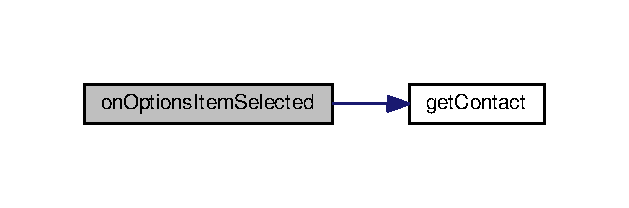
\includegraphics[width=302pt]{a00006_a37a55c533c74b60c0290ef1329d74e65_cgraph}
\end{center}
\end{figure}


\hypertarget{a00006_a1e3fee8580ec4092ffc6e3ce9d44f2b9}{\index{org\+::opensecurity\+::sms\+::view\+::\+Conversation\+Activity@{org\+::opensecurity\+::sms\+::view\+::\+Conversation\+Activity}!set\+Bubble\+Data@{set\+Bubble\+Data}}
\index{set\+Bubble\+Data@{set\+Bubble\+Data}!org\+::opensecurity\+::sms\+::view\+::\+Conversation\+Activity@{org\+::opensecurity\+::sms\+::view\+::\+Conversation\+Activity}}
\subsubsection[{set\+Bubble\+Data}]{\setlength{\rightskip}{0pt plus 5cm}void set\+Bubble\+Data (
\begin{DoxyParamCaption}
\item[{Array\+List$<$ {\bf Conversation\+Item} $>$}]{bubble\+Data}
\end{DoxyParamCaption}
)}}\label{a00006_a1e3fee8580ec4092ffc6e3ce9d44f2b9}
Just set the Array\+List of Bubbles in the activity. 
\begin{DoxyParams}{Parameters}
{\em bubble\+Data} & the data that we want to load \\
\hline
\end{DoxyParams}


Here is the call graph for this function\+:
\nopagebreak
\begin{figure}[H]
\begin{center}
\leavevmode
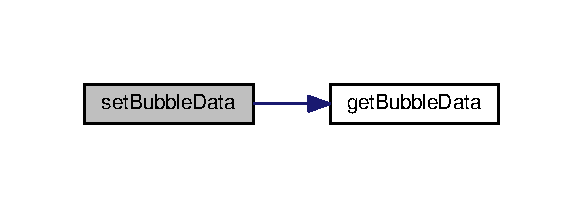
\includegraphics[width=280pt]{a00006_a1e3fee8580ec4092ffc6e3ce9d44f2b9_cgraph}
\end{center}
\end{figure}




Here is the caller graph for this function\+:
\nopagebreak
\begin{figure}[H]
\begin{center}
\leavevmode
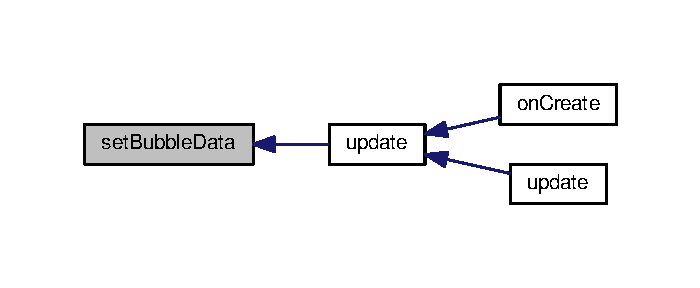
\includegraphics[width=336pt]{a00006_a1e3fee8580ec4092ffc6e3ce9d44f2b9_icgraph}
\end{center}
\end{figure}


\hypertarget{a00006_abef3c7b6635dc06ac6b8e4b37c51b37f}{\index{org\+::opensecurity\+::sms\+::view\+::\+Conversation\+Activity@{org\+::opensecurity\+::sms\+::view\+::\+Conversation\+Activity}!set\+Contact@{set\+Contact}}
\index{set\+Contact@{set\+Contact}!org\+::opensecurity\+::sms\+::view\+::\+Conversation\+Activity@{org\+::opensecurity\+::sms\+::view\+::\+Conversation\+Activity}}
\subsubsection[{set\+Contact}]{\setlength{\rightskip}{0pt plus 5cm}void set\+Contact (
\begin{DoxyParamCaption}
\item[{{\bf Contact}}]{contact}
\end{DoxyParamCaption}
)}}\label{a00006_abef3c7b6635dc06ac6b8e4b37c51b37f}
To set the current contact when we select it in previous activity 
\begin{DoxyParams}{Parameters}
{\em contact} & the future current contact of this activity conversation. \\
\hline
\end{DoxyParams}


Here is the caller graph for this function\+:
\nopagebreak
\begin{figure}[H]
\begin{center}
\leavevmode
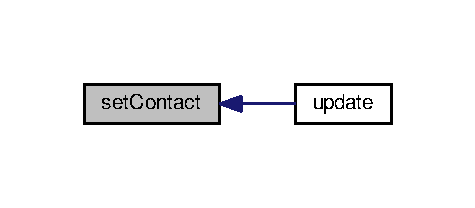
\includegraphics[width=228pt]{a00006_abef3c7b6635dc06ac6b8e4b37c51b37f_icgraph}
\end{center}
\end{figure}


\hypertarget{a00006_aa2825578f585a8a32958eaf0ce8df7b8}{\index{org\+::opensecurity\+::sms\+::view\+::\+Conversation\+Activity@{org\+::opensecurity\+::sms\+::view\+::\+Conversation\+Activity}!update@{update}}
\index{update@{update}!org\+::opensecurity\+::sms\+::view\+::\+Conversation\+Activity@{org\+::opensecurity\+::sms\+::view\+::\+Conversation\+Activity}}
\subsubsection[{update}]{\setlength{\rightskip}{0pt plus 5cm}void update (
\begin{DoxyParamCaption}
\item[{Intent}]{intent}
\end{DoxyParamCaption}
)}}\label{a00006_aa2825578f585a8a32958eaf0ce8df7b8}

\begin{DoxyParams}{Parameters}
{\em intent} & \\
\hline
\end{DoxyParams}


Here is the call graph for this function\+:
\nopagebreak
\begin{figure}[H]
\begin{center}
\leavevmode
\includegraphics[width=350pt]{a00006_aa2825578f585a8a32958eaf0ce8df7b8_cgraph}
\end{center}
\end{figure}


\hypertarget{a00006_ac5c54df7ed3b930268c8d7752c101725}{\index{org\+::opensecurity\+::sms\+::view\+::\+Conversation\+Activity@{org\+::opensecurity\+::sms\+::view\+::\+Conversation\+Activity}!update@{update}}
\index{update@{update}!org\+::opensecurity\+::sms\+::view\+::\+Conversation\+Activity@{org\+::opensecurity\+::sms\+::view\+::\+Conversation\+Activity}}
\subsubsection[{update}]{\setlength{\rightskip}{0pt plus 5cm}void update (
\begin{DoxyParamCaption}
{}
\end{DoxyParamCaption}
)}}\label{a00006_ac5c54df7ed3b930268c8d7752c101725}
This function is used to update a conversation when it's necessary 

Here is the call graph for this function\+:
\nopagebreak
\begin{figure}[H]
\begin{center}
\leavevmode
\includegraphics[width=350pt]{a00006_ac5c54df7ed3b930268c8d7752c101725_cgraph}
\end{center}
\end{figure}




Here is the caller graph for this function\+:
\nopagebreak
\begin{figure}[H]
\begin{center}
\leavevmode
\includegraphics[width=218pt]{a00006_ac5c54df7ed3b930268c8d7752c101725_icgraph}
\end{center}
\end{figure}




\subsection{Member Data Documentation}
\hypertarget{a00006_adaad4a865e59995c45ef2ad13f6e88a9}{\index{org\+::opensecurity\+::sms\+::view\+::\+Conversation\+Activity@{org\+::opensecurity\+::sms\+::view\+::\+Conversation\+Activity}!adapter@{adapter}}
\index{adapter@{adapter}!org\+::opensecurity\+::sms\+::view\+::\+Conversation\+Activity@{org\+::opensecurity\+::sms\+::view\+::\+Conversation\+Activity}}
\subsubsection[{adapter}]{\setlength{\rightskip}{0pt plus 5cm}{\bf Array\+Bubble\+Adapter} adapter\hspace{0.3cm}{\ttfamily [private]}}}\label{a00006_adaad4a865e59995c45ef2ad13f6e88a9}
The adapter for this activity \hypertarget{a00006_a68544a0bda28776dfb51718a3c71bf69}{\index{org\+::opensecurity\+::sms\+::view\+::\+Conversation\+Activity@{org\+::opensecurity\+::sms\+::view\+::\+Conversation\+Activity}!bubble\+Data@{bubble\+Data}}
\index{bubble\+Data@{bubble\+Data}!org\+::opensecurity\+::sms\+::view\+::\+Conversation\+Activity@{org\+::opensecurity\+::sms\+::view\+::\+Conversation\+Activity}}
\subsubsection[{bubble\+Data}]{\setlength{\rightskip}{0pt plus 5cm}Array\+List$<${\bf Conversation\+Item}$>$ bubble\+Data\hspace{0.3cm}{\ttfamily [private]}}}\label{a00006_a68544a0bda28776dfb51718a3c71bf69}
The array to keep bubbles. We load messages into this array \hypertarget{a00006_ae5bb074a89738fa417e643960b0041c6}{\index{org\+::opensecurity\+::sms\+::view\+::\+Conversation\+Activity@{org\+::opensecurity\+::sms\+::view\+::\+Conversation\+Activity}!bubble\+List@{bubble\+List}}
\index{bubble\+List@{bubble\+List}!org\+::opensecurity\+::sms\+::view\+::\+Conversation\+Activity@{org\+::opensecurity\+::sms\+::view\+::\+Conversation\+Activity}}
\subsubsection[{bubble\+List}]{\setlength{\rightskip}{0pt plus 5cm}Swipe\+Menu\+List\+View bubble\+List\hspace{0.3cm}{\ttfamily [private]}}}\label{a00006_ae5bb074a89738fa417e643960b0041c6}
The liste\+View for displaying bubbles \hypertarget{a00006_a3459849ab29ad684658dbcd0cf8c5d5a}{\index{org\+::opensecurity\+::sms\+::view\+::\+Conversation\+Activity@{org\+::opensecurity\+::sms\+::view\+::\+Conversation\+Activity}!contact@{contact}}
\index{contact@{contact}!org\+::opensecurity\+::sms\+::view\+::\+Conversation\+Activity@{org\+::opensecurity\+::sms\+::view\+::\+Conversation\+Activity}}
\subsubsection[{contact}]{\setlength{\rightskip}{0pt plus 5cm}{\bf Contact} contact\hspace{0.3cm}{\ttfamily [private]}}}\label{a00006_a3459849ab29ad684658dbcd0cf8c5d5a}
The contact who has been selected in conversation activity \hypertarget{a00006_a64a39fb2b7f756356462736dfbdb9f9f}{\index{org\+::opensecurity\+::sms\+::view\+::\+Conversation\+Activity@{org\+::opensecurity\+::sms\+::view\+::\+Conversation\+Activity}!instance@{instance}}
\index{instance@{instance}!org\+::opensecurity\+::sms\+::view\+::\+Conversation\+Activity@{org\+::opensecurity\+::sms\+::view\+::\+Conversation\+Activity}}
\subsubsection[{instance}]{\setlength{\rightskip}{0pt plus 5cm}{\bf Conversation\+Activity} instance\hspace{0.3cm}{\ttfamily [static]}, {\ttfamily [private]}}}\label{a00006_a64a39fb2b7f756356462736dfbdb9f9f}
instance of a conversation activity \hypertarget{a00006_a2e4d147a434708e05027f41ecf9ed577}{\index{org\+::opensecurity\+::sms\+::view\+::\+Conversation\+Activity@{org\+::opensecurity\+::sms\+::view\+::\+Conversation\+Activity}!send\+Button@{send\+Button}}
\index{send\+Button@{send\+Button}!org\+::opensecurity\+::sms\+::view\+::\+Conversation\+Activity@{org\+::opensecurity\+::sms\+::view\+::\+Conversation\+Activity}}
\subsubsection[{send\+Button}]{\setlength{\rightskip}{0pt plus 5cm}Button send\+Button\hspace{0.3cm}{\ttfamily [private]}}}\label{a00006_a2e4d147a434708e05027f41ecf9ed577}
the button used to send messages \hypertarget{a00006_abc418be8d11246756bfcb7f95123a88d}{\index{org\+::opensecurity\+::sms\+::view\+::\+Conversation\+Activity@{org\+::opensecurity\+::sms\+::view\+::\+Conversation\+Activity}!text\+Message@{text\+Message}}
\index{text\+Message@{text\+Message}!org\+::opensecurity\+::sms\+::view\+::\+Conversation\+Activity@{org\+::opensecurity\+::sms\+::view\+::\+Conversation\+Activity}}
\subsubsection[{text\+Message}]{\setlength{\rightskip}{0pt plus 5cm}Edit\+Text text\+Message\hspace{0.3cm}{\ttfamily [private]}}}\label{a00006_abc418be8d11246756bfcb7f95123a88d}
The edit\+Text wiget to enter text to send 

The documentation for this class was generated from the following file\+:\begin{DoxyCompactItemize}
\item 
app/src/main/java/org/opensecurity/sms/view/\hyperlink{a00030}{Conversation\+Activity.\+java}\end{DoxyCompactItemize}

\hypertarget{a00007}{\section{Conversation\+Activity Class Reference}
\label{a00007}\index{Conversation\+Activity@{Conversation\+Activity}}
}


Inheritance diagram for Conversation\+Activity\+:
\nopagebreak
\begin{figure}[H]
\begin{center}
\leavevmode
\includegraphics[width=214pt]{a00074}
\end{center}
\end{figure}


Collaboration diagram for Conversation\+Activity\+:
\nopagebreak
\begin{figure}[H]
\begin{center}
\leavevmode
\includegraphics[width=350pt]{a00075}
\end{center}
\end{figure}
\subsection*{Public Member Functions}
\begin{DoxyCompactItemize}
\item 
boolean \hyperlink{a00007_a8f7d87763ddaf085205a54e8477ecfce}{on\+Create\+Options\+Menu} (Menu menu)
\item 
boolean \hyperlink{a00007_a37a55c533c74b60c0290ef1329d74e65}{on\+Options\+Item\+Selected} (Menu\+Item item)
\item 
void \hyperlink{a00007_a92b8e0730130e1184a8cdbd89590779d}{listeners} ()
\item 
void \hyperlink{a00007_a1e3fee8580ec4092ffc6e3ce9d44f2b9}{set\+Bubble\+Data} (Array\+List$<$ \hyperlink{a00008}{Conversation\+Item} $>$ \hyperlink{a00007_a68544a0bda28776dfb51718a3c71bf69}{bubble\+Data})
\item 
Array\+List$<$ \hyperlink{a00008}{Conversation\+Item} $>$ \hyperlink{a00007_ac8e14177e6079becbb8bc1f8b35197e0}{get\+Bubble\+Data} ()
\item 
Swipe\+Menu\+List\+View \hyperlink{a00007_af293d3ea5f145650e06a96d2bae482da}{get\+Bubble\+List} ()
\item 
Button \hyperlink{a00007_a57576f3fc93bfa5a685ed5ee30fe113c}{get\+Send\+Button} ()
\item 
\hyperlink{a00005}{Contact} \hyperlink{a00007_adb647c7ae09f1d5755db63d701968925}{get\+Contact} ()
\item 
void \hyperlink{a00007_abef3c7b6635dc06ac6b8e4b37c51b37f}{set\+Contact} (\hyperlink{a00005}{Contact} \hyperlink{a00007_a3459849ab29ad684658dbcd0cf8c5d5a}{contact})
\item 
void \hyperlink{a00007_aa2825578f585a8a32958eaf0ce8df7b8}{update} (Intent intent)
\item 
void \hyperlink{a00007_ac5c54df7ed3b930268c8d7752c101725}{update} ()
\item 
\hyperlink{a00002}{Array\+Bubble\+Adapter} \hyperlink{a00007_a06738816ea7799569af8fa119bb49f7e}{get\+Adapter} ()
\end{DoxyCompactItemize}
\subsection*{Static Public Member Functions}
\begin{DoxyCompactItemize}
\item 
static \hyperlink{a00007}{Conversation\+Activity} \hyperlink{a00007_a7ebafa56e442a2f16c4afe044e65695b}{get\+Instance} ()
\end{DoxyCompactItemize}
\subsection*{Protected Member Functions}
\begin{DoxyCompactItemize}
\item 
void \hyperlink{a00007_a85e87cb5ced88dff7c8173ecc4f636d1}{on\+Create} (Bundle saved\+Instance\+State)
\end{DoxyCompactItemize}
\subsection*{Private Attributes}
\begin{DoxyCompactItemize}
\item 
\hyperlink{a00005}{Contact} \hyperlink{a00007_a3459849ab29ad684658dbcd0cf8c5d5a}{contact}
\item 
Array\+List$<$ \hyperlink{a00008}{Conversation\+Item} $>$ \hyperlink{a00007_a68544a0bda28776dfb51718a3c71bf69}{bubble\+Data}
\item 
\hyperlink{a00002}{Array\+Bubble\+Adapter} \hyperlink{a00007_adaad4a865e59995c45ef2ad13f6e88a9}{adapter}
\item 
Swipe\+Menu\+List\+View \hyperlink{a00007_ae5bb074a89738fa417e643960b0041c6}{bubble\+List}
\item 
Edit\+Text \hyperlink{a00007_abc418be8d11246756bfcb7f95123a88d}{text\+Message}
\item 
Button \hyperlink{a00007_a2e4d147a434708e05027f41ecf9ed577}{send\+Button}
\end{DoxyCompactItemize}
\subsection*{Static Private Attributes}
\begin{DoxyCompactItemize}
\item 
static \hyperlink{a00007}{Conversation\+Activity} \hyperlink{a00007_a64a39fb2b7f756356462736dfbdb9f9f}{instance}
\end{DoxyCompactItemize}


\subsection{Detailed Description}
This class is an activity for displaying one conversation bitween us and another contact. 

\subsection{Member Function Documentation}
\hypertarget{a00007_a06738816ea7799569af8fa119bb49f7e}{\index{org\+::opensecurity\+::sms\+::view\+::\+Conversation\+Activity@{org\+::opensecurity\+::sms\+::view\+::\+Conversation\+Activity}!get\+Adapter@{get\+Adapter}}
\index{get\+Adapter@{get\+Adapter}!org\+::opensecurity\+::sms\+::view\+::\+Conversation\+Activity@{org\+::opensecurity\+::sms\+::view\+::\+Conversation\+Activity}}
\subsubsection[{get\+Adapter}]{\setlength{\rightskip}{0pt plus 5cm}{\bf Array\+Bubble\+Adapter} get\+Adapter (
\begin{DoxyParamCaption}
{}
\end{DoxyParamCaption}
)}}\label{a00007_a06738816ea7799569af8fa119bb49f7e}
To get the adapter (design) \begin{DoxyReturn}{Returns}
the adapter of current activity 
\end{DoxyReturn}


Here is the caller graph for this function\+:
\nopagebreak
\begin{figure}[H]
\begin{center}
\leavevmode
\includegraphics[width=236pt]{a00007_a06738816ea7799569af8fa119bb49f7e_icgraph}
\end{center}
\end{figure}


\hypertarget{a00007_ac8e14177e6079becbb8bc1f8b35197e0}{\index{org\+::opensecurity\+::sms\+::view\+::\+Conversation\+Activity@{org\+::opensecurity\+::sms\+::view\+::\+Conversation\+Activity}!get\+Bubble\+Data@{get\+Bubble\+Data}}
\index{get\+Bubble\+Data@{get\+Bubble\+Data}!org\+::opensecurity\+::sms\+::view\+::\+Conversation\+Activity@{org\+::opensecurity\+::sms\+::view\+::\+Conversation\+Activity}}
\subsubsection[{get\+Bubble\+Data}]{\setlength{\rightskip}{0pt plus 5cm}Array\+List$<${\bf Conversation\+Item}$>$ get\+Bubble\+Data (
\begin{DoxyParamCaption}
{}
\end{DoxyParamCaption}
)}}\label{a00007_ac8e14177e6079becbb8bc1f8b35197e0}
Just return the bubble\+Data which are loaded in the activity \begin{DoxyReturn}{Returns}
bubble\+Data of current activity 
\end{DoxyReturn}


Here is the caller graph for this function\+:
\nopagebreak
\begin{figure}[H]
\begin{center}
\leavevmode
\includegraphics[width=350pt]{a00007_ac8e14177e6079becbb8bc1f8b35197e0_icgraph}
\end{center}
\end{figure}


\hypertarget{a00007_af293d3ea5f145650e06a96d2bae482da}{\index{org\+::opensecurity\+::sms\+::view\+::\+Conversation\+Activity@{org\+::opensecurity\+::sms\+::view\+::\+Conversation\+Activity}!get\+Bubble\+List@{get\+Bubble\+List}}
\index{get\+Bubble\+List@{get\+Bubble\+List}!org\+::opensecurity\+::sms\+::view\+::\+Conversation\+Activity@{org\+::opensecurity\+::sms\+::view\+::\+Conversation\+Activity}}
\subsubsection[{get\+Bubble\+List}]{\setlength{\rightskip}{0pt plus 5cm}Swipe\+Menu\+List\+View get\+Bubble\+List (
\begin{DoxyParamCaption}
{}
\end{DoxyParamCaption}
)}}\label{a00007_af293d3ea5f145650e06a96d2bae482da}
To return the menu\+List\+View of bubbles. \begin{DoxyReturn}{Returns}
the List\+View of current activity 
\end{DoxyReturn}


Here is the caller graph for this function\+:
\nopagebreak
\begin{figure}[H]
\begin{center}
\leavevmode
\includegraphics[width=248pt]{a00007_af293d3ea5f145650e06a96d2bae482da_icgraph}
\end{center}
\end{figure}


\hypertarget{a00007_adb647c7ae09f1d5755db63d701968925}{\index{org\+::opensecurity\+::sms\+::view\+::\+Conversation\+Activity@{org\+::opensecurity\+::sms\+::view\+::\+Conversation\+Activity}!get\+Contact@{get\+Contact}}
\index{get\+Contact@{get\+Contact}!org\+::opensecurity\+::sms\+::view\+::\+Conversation\+Activity@{org\+::opensecurity\+::sms\+::view\+::\+Conversation\+Activity}}
\subsubsection[{get\+Contact}]{\setlength{\rightskip}{0pt plus 5cm}{\bf Contact} get\+Contact (
\begin{DoxyParamCaption}
{}
\end{DoxyParamCaption}
)}}\label{a00007_adb647c7ae09f1d5755db63d701968925}
To get the contact of our current activity. \begin{DoxyReturn}{Returns}
the current contact of selected activity conversation 
\end{DoxyReturn}


Here is the caller graph for this function\+:
\nopagebreak
\begin{figure}[H]
\begin{center}
\leavevmode
\includegraphics[width=350pt]{a00007_adb647c7ae09f1d5755db63d701968925_icgraph}
\end{center}
\end{figure}


\hypertarget{a00007_a7ebafa56e442a2f16c4afe044e65695b}{\index{org\+::opensecurity\+::sms\+::view\+::\+Conversation\+Activity@{org\+::opensecurity\+::sms\+::view\+::\+Conversation\+Activity}!get\+Instance@{get\+Instance}}
\index{get\+Instance@{get\+Instance}!org\+::opensecurity\+::sms\+::view\+::\+Conversation\+Activity@{org\+::opensecurity\+::sms\+::view\+::\+Conversation\+Activity}}
\subsubsection[{get\+Instance}]{\setlength{\rightskip}{0pt plus 5cm}static {\bf Conversation\+Activity} get\+Instance (
\begin{DoxyParamCaption}
{}
\end{DoxyParamCaption}
)\hspace{0.3cm}{\ttfamily [static]}}}\label{a00007_a7ebafa56e442a2f16c4afe044e65695b}
To return the current instance. Be sure that is the only one instance (singleton pattern) \begin{DoxyReturn}{Returns}
the instance of current activity (=this) 
\end{DoxyReturn}


Here is the caller graph for this function\+:
\nopagebreak
\begin{figure}[H]
\begin{center}
\leavevmode
\includegraphics[width=328pt]{a00007_a7ebafa56e442a2f16c4afe044e65695b_icgraph}
\end{center}
\end{figure}


\hypertarget{a00007_a57576f3fc93bfa5a685ed5ee30fe113c}{\index{org\+::opensecurity\+::sms\+::view\+::\+Conversation\+Activity@{org\+::opensecurity\+::sms\+::view\+::\+Conversation\+Activity}!get\+Send\+Button@{get\+Send\+Button}}
\index{get\+Send\+Button@{get\+Send\+Button}!org\+::opensecurity\+::sms\+::view\+::\+Conversation\+Activity@{org\+::opensecurity\+::sms\+::view\+::\+Conversation\+Activity}}
\subsubsection[{get\+Send\+Button}]{\setlength{\rightskip}{0pt plus 5cm}Button get\+Send\+Button (
\begin{DoxyParamCaption}
{}
\end{DoxyParamCaption}
)}}\label{a00007_a57576f3fc93bfa5a685ed5ee30fe113c}
To return the send\+Button of this activity. \begin{DoxyReturn}{Returns}
the Button to send messages in this activity 
\end{DoxyReturn}


Here is the caller graph for this function\+:
\nopagebreak
\begin{figure}[H]
\begin{center}
\leavevmode
\includegraphics[width=344pt]{a00007_a57576f3fc93bfa5a685ed5ee30fe113c_icgraph}
\end{center}
\end{figure}


\hypertarget{a00007_a92b8e0730130e1184a8cdbd89590779d}{\index{org\+::opensecurity\+::sms\+::view\+::\+Conversation\+Activity@{org\+::opensecurity\+::sms\+::view\+::\+Conversation\+Activity}!listeners@{listeners}}
\index{listeners@{listeners}!org\+::opensecurity\+::sms\+::view\+::\+Conversation\+Activity@{org\+::opensecurity\+::sms\+::view\+::\+Conversation\+Activity}}
\subsubsection[{listeners}]{\setlength{\rightskip}{0pt plus 5cm}void listeners (
\begin{DoxyParamCaption}
{}
\end{DoxyParamCaption}
)}}\label{a00007_a92b8e0730130e1184a8cdbd89590779d}
contains listeners of the activity First listener. We call send\+S\+M\+S function and after that, if the sms exists, we create a new bubble and we reload the Adapter.

Here is the call graph for this function\+:
\nopagebreak
\begin{figure}[H]
\begin{center}
\leavevmode
\includegraphics[width=326pt]{a00007_a92b8e0730130e1184a8cdbd89590779d_cgraph}
\end{center}
\end{figure}




Here is the caller graph for this function\+:
\nopagebreak
\begin{figure}[H]
\begin{center}
\leavevmode
\includegraphics[width=226pt]{a00007_a92b8e0730130e1184a8cdbd89590779d_icgraph}
\end{center}
\end{figure}


\hypertarget{a00007_a85e87cb5ced88dff7c8173ecc4f636d1}{\index{org\+::opensecurity\+::sms\+::view\+::\+Conversation\+Activity@{org\+::opensecurity\+::sms\+::view\+::\+Conversation\+Activity}!on\+Create@{on\+Create}}
\index{on\+Create@{on\+Create}!org\+::opensecurity\+::sms\+::view\+::\+Conversation\+Activity@{org\+::opensecurity\+::sms\+::view\+::\+Conversation\+Activity}}
\subsubsection[{on\+Create}]{\setlength{\rightskip}{0pt plus 5cm}void on\+Create (
\begin{DoxyParamCaption}
\item[{Bundle}]{saved\+Instance\+State}
\end{DoxyParamCaption}
)\hspace{0.3cm}{\ttfamily [protected]}}}\label{a00007_a85e87cb5ced88dff7c8173ecc4f636d1}
To create the activity


\begin{DoxyParams}{Parameters}
{\em saved\+Instance\+State} & save the instance state to keep informations. \\
\hline
\end{DoxyParams}


Here is the call graph for this function\+:
\nopagebreak
\begin{figure}[H]
\begin{center}
\leavevmode
\includegraphics[width=350pt]{a00007_a85e87cb5ced88dff7c8173ecc4f636d1_cgraph}
\end{center}
\end{figure}


\hypertarget{a00007_a8f7d87763ddaf085205a54e8477ecfce}{\index{org\+::opensecurity\+::sms\+::view\+::\+Conversation\+Activity@{org\+::opensecurity\+::sms\+::view\+::\+Conversation\+Activity}!on\+Create\+Options\+Menu@{on\+Create\+Options\+Menu}}
\index{on\+Create\+Options\+Menu@{on\+Create\+Options\+Menu}!org\+::opensecurity\+::sms\+::view\+::\+Conversation\+Activity@{org\+::opensecurity\+::sms\+::view\+::\+Conversation\+Activity}}
\subsubsection[{on\+Create\+Options\+Menu}]{\setlength{\rightskip}{0pt plus 5cm}boolean on\+Create\+Options\+Menu (
\begin{DoxyParamCaption}
\item[{Menu}]{menu}
\end{DoxyParamCaption}
)}}\label{a00007_a8f7d87763ddaf085205a54e8477ecfce}
Use to create an option\+Menu.


\begin{DoxyParams}{Parameters}
{\em menu} & keep informations relative to the menu \\
\hline
\end{DoxyParams}
\begin{DoxyReturn}{Returns}
boolean if the menu is create or no 
\end{DoxyReturn}


Here is the call graph for this function\+:
\nopagebreak
\begin{figure}[H]
\begin{center}
\leavevmode
\includegraphics[width=296pt]{a00007_a8f7d87763ddaf085205a54e8477ecfce_cgraph}
\end{center}
\end{figure}


\hypertarget{a00007_a37a55c533c74b60c0290ef1329d74e65}{\index{org\+::opensecurity\+::sms\+::view\+::\+Conversation\+Activity@{org\+::opensecurity\+::sms\+::view\+::\+Conversation\+Activity}!on\+Options\+Item\+Selected@{on\+Options\+Item\+Selected}}
\index{on\+Options\+Item\+Selected@{on\+Options\+Item\+Selected}!org\+::opensecurity\+::sms\+::view\+::\+Conversation\+Activity@{org\+::opensecurity\+::sms\+::view\+::\+Conversation\+Activity}}
\subsubsection[{on\+Options\+Item\+Selected}]{\setlength{\rightskip}{0pt plus 5cm}boolean on\+Options\+Item\+Selected (
\begin{DoxyParamCaption}
\item[{Menu\+Item}]{item}
\end{DoxyParamCaption}
)}}\label{a00007_a37a55c533c74b60c0290ef1329d74e65}
To react when we select on item on the menu. 
\begin{DoxyParams}{Parameters}
{\em item} & the current selected item. \\
\hline
\end{DoxyParams}
\begin{DoxyReturn}{Returns}

\end{DoxyReturn}


Here is the call graph for this function\+:
\nopagebreak
\begin{figure}[H]
\begin{center}
\leavevmode
\includegraphics[width=302pt]{a00007_a37a55c533c74b60c0290ef1329d74e65_cgraph}
\end{center}
\end{figure}


\hypertarget{a00007_a1e3fee8580ec4092ffc6e3ce9d44f2b9}{\index{org\+::opensecurity\+::sms\+::view\+::\+Conversation\+Activity@{org\+::opensecurity\+::sms\+::view\+::\+Conversation\+Activity}!set\+Bubble\+Data@{set\+Bubble\+Data}}
\index{set\+Bubble\+Data@{set\+Bubble\+Data}!org\+::opensecurity\+::sms\+::view\+::\+Conversation\+Activity@{org\+::opensecurity\+::sms\+::view\+::\+Conversation\+Activity}}
\subsubsection[{set\+Bubble\+Data}]{\setlength{\rightskip}{0pt plus 5cm}void set\+Bubble\+Data (
\begin{DoxyParamCaption}
\item[{Array\+List$<$ {\bf Conversation\+Item} $>$}]{bubble\+Data}
\end{DoxyParamCaption}
)}}\label{a00007_a1e3fee8580ec4092ffc6e3ce9d44f2b9}
Just set the Array\+List of Bubbles in the activity. 
\begin{DoxyParams}{Parameters}
{\em bubble\+Data} & the data that we want to load \\
\hline
\end{DoxyParams}


Here is the call graph for this function\+:
\nopagebreak
\begin{figure}[H]
\begin{center}
\leavevmode
\includegraphics[width=280pt]{a00007_a1e3fee8580ec4092ffc6e3ce9d44f2b9_cgraph}
\end{center}
\end{figure}




Here is the caller graph for this function\+:
\nopagebreak
\begin{figure}[H]
\begin{center}
\leavevmode
\includegraphics[width=336pt]{a00007_a1e3fee8580ec4092ffc6e3ce9d44f2b9_icgraph}
\end{center}
\end{figure}


\hypertarget{a00007_abef3c7b6635dc06ac6b8e4b37c51b37f}{\index{org\+::opensecurity\+::sms\+::view\+::\+Conversation\+Activity@{org\+::opensecurity\+::sms\+::view\+::\+Conversation\+Activity}!set\+Contact@{set\+Contact}}
\index{set\+Contact@{set\+Contact}!org\+::opensecurity\+::sms\+::view\+::\+Conversation\+Activity@{org\+::opensecurity\+::sms\+::view\+::\+Conversation\+Activity}}
\subsubsection[{set\+Contact}]{\setlength{\rightskip}{0pt plus 5cm}void set\+Contact (
\begin{DoxyParamCaption}
\item[{{\bf Contact}}]{contact}
\end{DoxyParamCaption}
)}}\label{a00007_abef3c7b6635dc06ac6b8e4b37c51b37f}
To set the current contact when we select it in previous activity 
\begin{DoxyParams}{Parameters}
{\em contact} & the future current contact of this activity conversation. \\
\hline
\end{DoxyParams}


Here is the caller graph for this function\+:
\nopagebreak
\begin{figure}[H]
\begin{center}
\leavevmode
\includegraphics[width=228pt]{a00007_abef3c7b6635dc06ac6b8e4b37c51b37f_icgraph}
\end{center}
\end{figure}


\hypertarget{a00007_aa2825578f585a8a32958eaf0ce8df7b8}{\index{org\+::opensecurity\+::sms\+::view\+::\+Conversation\+Activity@{org\+::opensecurity\+::sms\+::view\+::\+Conversation\+Activity}!update@{update}}
\index{update@{update}!org\+::opensecurity\+::sms\+::view\+::\+Conversation\+Activity@{org\+::opensecurity\+::sms\+::view\+::\+Conversation\+Activity}}
\subsubsection[{update}]{\setlength{\rightskip}{0pt plus 5cm}void update (
\begin{DoxyParamCaption}
\item[{Intent}]{intent}
\end{DoxyParamCaption}
)}}\label{a00007_aa2825578f585a8a32958eaf0ce8df7b8}

\begin{DoxyParams}{Parameters}
{\em intent} & \\
\hline
\end{DoxyParams}


Here is the call graph for this function\+:
\nopagebreak
\begin{figure}[H]
\begin{center}
\leavevmode
\includegraphics[width=350pt]{a00007_aa2825578f585a8a32958eaf0ce8df7b8_cgraph}
\end{center}
\end{figure}


\hypertarget{a00007_ac5c54df7ed3b930268c8d7752c101725}{\index{org\+::opensecurity\+::sms\+::view\+::\+Conversation\+Activity@{org\+::opensecurity\+::sms\+::view\+::\+Conversation\+Activity}!update@{update}}
\index{update@{update}!org\+::opensecurity\+::sms\+::view\+::\+Conversation\+Activity@{org\+::opensecurity\+::sms\+::view\+::\+Conversation\+Activity}}
\subsubsection[{update}]{\setlength{\rightskip}{0pt plus 5cm}void update (
\begin{DoxyParamCaption}
{}
\end{DoxyParamCaption}
)}}\label{a00007_ac5c54df7ed3b930268c8d7752c101725}
This function is used to update a conversation when it's necessary 

Here is the call graph for this function\+:
\nopagebreak
\begin{figure}[H]
\begin{center}
\leavevmode
\includegraphics[width=350pt]{a00007_ac5c54df7ed3b930268c8d7752c101725_cgraph}
\end{center}
\end{figure}




Here is the caller graph for this function\+:
\nopagebreak
\begin{figure}[H]
\begin{center}
\leavevmode
\includegraphics[width=218pt]{a00007_ac5c54df7ed3b930268c8d7752c101725_icgraph}
\end{center}
\end{figure}




\subsection{Member Data Documentation}
\hypertarget{a00007_adaad4a865e59995c45ef2ad13f6e88a9}{\index{org\+::opensecurity\+::sms\+::view\+::\+Conversation\+Activity@{org\+::opensecurity\+::sms\+::view\+::\+Conversation\+Activity}!adapter@{adapter}}
\index{adapter@{adapter}!org\+::opensecurity\+::sms\+::view\+::\+Conversation\+Activity@{org\+::opensecurity\+::sms\+::view\+::\+Conversation\+Activity}}
\subsubsection[{adapter}]{\setlength{\rightskip}{0pt plus 5cm}{\bf Array\+Bubble\+Adapter} adapter\hspace{0.3cm}{\ttfamily [private]}}}\label{a00007_adaad4a865e59995c45ef2ad13f6e88a9}
The adapter for this activity \hypertarget{a00007_a68544a0bda28776dfb51718a3c71bf69}{\index{org\+::opensecurity\+::sms\+::view\+::\+Conversation\+Activity@{org\+::opensecurity\+::sms\+::view\+::\+Conversation\+Activity}!bubble\+Data@{bubble\+Data}}
\index{bubble\+Data@{bubble\+Data}!org\+::opensecurity\+::sms\+::view\+::\+Conversation\+Activity@{org\+::opensecurity\+::sms\+::view\+::\+Conversation\+Activity}}
\subsubsection[{bubble\+Data}]{\setlength{\rightskip}{0pt plus 5cm}Array\+List$<${\bf Conversation\+Item}$>$ bubble\+Data\hspace{0.3cm}{\ttfamily [private]}}}\label{a00007_a68544a0bda28776dfb51718a3c71bf69}
The array to keep bubbles. We load messages into this array \hypertarget{a00007_ae5bb074a89738fa417e643960b0041c6}{\index{org\+::opensecurity\+::sms\+::view\+::\+Conversation\+Activity@{org\+::opensecurity\+::sms\+::view\+::\+Conversation\+Activity}!bubble\+List@{bubble\+List}}
\index{bubble\+List@{bubble\+List}!org\+::opensecurity\+::sms\+::view\+::\+Conversation\+Activity@{org\+::opensecurity\+::sms\+::view\+::\+Conversation\+Activity}}
\subsubsection[{bubble\+List}]{\setlength{\rightskip}{0pt plus 5cm}Swipe\+Menu\+List\+View bubble\+List\hspace{0.3cm}{\ttfamily [private]}}}\label{a00007_ae5bb074a89738fa417e643960b0041c6}
The liste\+View for displaying bubbles \hypertarget{a00007_a3459849ab29ad684658dbcd0cf8c5d5a}{\index{org\+::opensecurity\+::sms\+::view\+::\+Conversation\+Activity@{org\+::opensecurity\+::sms\+::view\+::\+Conversation\+Activity}!contact@{contact}}
\index{contact@{contact}!org\+::opensecurity\+::sms\+::view\+::\+Conversation\+Activity@{org\+::opensecurity\+::sms\+::view\+::\+Conversation\+Activity}}
\subsubsection[{contact}]{\setlength{\rightskip}{0pt plus 5cm}{\bf Contact} contact\hspace{0.3cm}{\ttfamily [private]}}}\label{a00007_a3459849ab29ad684658dbcd0cf8c5d5a}
The contact who has been selected in conversation activity \hypertarget{a00007_a64a39fb2b7f756356462736dfbdb9f9f}{\index{org\+::opensecurity\+::sms\+::view\+::\+Conversation\+Activity@{org\+::opensecurity\+::sms\+::view\+::\+Conversation\+Activity}!instance@{instance}}
\index{instance@{instance}!org\+::opensecurity\+::sms\+::view\+::\+Conversation\+Activity@{org\+::opensecurity\+::sms\+::view\+::\+Conversation\+Activity}}
\subsubsection[{instance}]{\setlength{\rightskip}{0pt plus 5cm}{\bf Conversation\+Activity} instance\hspace{0.3cm}{\ttfamily [static]}, {\ttfamily [private]}}}\label{a00007_a64a39fb2b7f756356462736dfbdb9f9f}
instance of a conversation activity \hypertarget{a00007_a2e4d147a434708e05027f41ecf9ed577}{\index{org\+::opensecurity\+::sms\+::view\+::\+Conversation\+Activity@{org\+::opensecurity\+::sms\+::view\+::\+Conversation\+Activity}!send\+Button@{send\+Button}}
\index{send\+Button@{send\+Button}!org\+::opensecurity\+::sms\+::view\+::\+Conversation\+Activity@{org\+::opensecurity\+::sms\+::view\+::\+Conversation\+Activity}}
\subsubsection[{send\+Button}]{\setlength{\rightskip}{0pt plus 5cm}Button send\+Button\hspace{0.3cm}{\ttfamily [private]}}}\label{a00007_a2e4d147a434708e05027f41ecf9ed577}
the button used to send messages \hypertarget{a00007_abc418be8d11246756bfcb7f95123a88d}{\index{org\+::opensecurity\+::sms\+::view\+::\+Conversation\+Activity@{org\+::opensecurity\+::sms\+::view\+::\+Conversation\+Activity}!text\+Message@{text\+Message}}
\index{text\+Message@{text\+Message}!org\+::opensecurity\+::sms\+::view\+::\+Conversation\+Activity@{org\+::opensecurity\+::sms\+::view\+::\+Conversation\+Activity}}
\subsubsection[{text\+Message}]{\setlength{\rightskip}{0pt plus 5cm}Edit\+Text text\+Message\hspace{0.3cm}{\ttfamily [private]}}}\label{a00007_abc418be8d11246756bfcb7f95123a88d}
The edit\+Text wiget to enter text to send 

The documentation for this class was generated from the following file\+:\begin{DoxyCompactItemize}
\item 
app/src/main/java/org/opensecurity/sms/view/\hyperlink{a00028}{Conversation\+Activity.\+java}\end{DoxyCompactItemize}

\hypertarget{a00008}{\section{Conversation\+Item Class Reference}
\label{a00008}\index{Conversation\+Item@{Conversation\+Item}}
}


Inheritance diagram for Conversation\+Item\+:
\nopagebreak
\begin{figure}[H]
\begin{center}
\leavevmode
\includegraphics[width=198pt]{a00058}
\end{center}
\end{figure}


Collaboration diagram for Conversation\+Item\+:
\nopagebreak
\begin{figure}[H]
\begin{center}
\leavevmode
\includegraphics[width=198pt]{a00059}
\end{center}
\end{figure}
\subsection*{Public Member Functions}
\begin{DoxyCompactItemize}
\item 
\hyperlink{a00008_ae50f1143e886a4a835296609372ec04a}{Conversation\+Item} (Calendar \hyperlink{a00008_aa713d1025d73543bd4eae313a1868570}{date})
\item 
Calendar \hyperlink{a00008_a91855ab66a4bb5c5e62f947170f29b10}{get\+Date} ()
\item 
String \hyperlink{a00008_aa53441954dd0352c8b8964194365c688}{get\+Managed\+Date} ()
\item 
boolean \hyperlink{a00008_abadf98014647b41c6a96847158d24230}{has\+To\+Managed\+Date} (Calendar \hyperlink{a00008_aa713d1025d73543bd4eae313a1868570}{date})
\item 
void \hyperlink{a00008_a65c1a5dad9225d01d585af72e0c80138}{set\+Date} (Calendar \hyperlink{a00008_aa713d1025d73543bd4eae313a1868570}{date})
\end{DoxyCompactItemize}
\subsection*{Private Attributes}
\begin{DoxyCompactItemize}
\item 
Calendar \hyperlink{a00008_aa713d1025d73543bd4eae313a1868570}{date}
\end{DoxyCompactItemize}


\subsection{Detailed Description}
A class to keep a date of message provided from one bubble. A mother class from \hyperlink{a00004}{Bubble} 

\subsection{Constructor \& Destructor Documentation}
\hypertarget{a00008_ae50f1143e886a4a835296609372ec04a}{\index{org\+::opensecurity\+::sms\+::model\+::model\+View\+::conversation\+::\+Conversation\+Item@{org\+::opensecurity\+::sms\+::model\+::model\+View\+::conversation\+::\+Conversation\+Item}!Conversation\+Item@{Conversation\+Item}}
\index{Conversation\+Item@{Conversation\+Item}!org\+::opensecurity\+::sms\+::model\+::model\+View\+::conversation\+::\+Conversation\+Item@{org\+::opensecurity\+::sms\+::model\+::model\+View\+::conversation\+::\+Conversation\+Item}}
\subsubsection[{Conversation\+Item}]{\setlength{\rightskip}{0pt plus 5cm}{\bf Conversation\+Item} (
\begin{DoxyParamCaption}
\item[{Calendar}]{date}
\end{DoxyParamCaption}
)}}\label{a00008_ae50f1143e886a4a835296609372ec04a}
constructor 
\begin{DoxyParams}{Parameters}
{\em date} & the date of a message \\
\hline
\end{DoxyParams}


Here is the call graph for this function\+:
\nopagebreak
\begin{figure}[H]
\begin{center}
\leavevmode
\includegraphics[width=262pt]{a00008_ae50f1143e886a4a835296609372ec04a_cgraph}
\end{center}
\end{figure}




\subsection{Member Function Documentation}
\hypertarget{a00008_a91855ab66a4bb5c5e62f947170f29b10}{\index{org\+::opensecurity\+::sms\+::model\+::model\+View\+::conversation\+::\+Conversation\+Item@{org\+::opensecurity\+::sms\+::model\+::model\+View\+::conversation\+::\+Conversation\+Item}!get\+Date@{get\+Date}}
\index{get\+Date@{get\+Date}!org\+::opensecurity\+::sms\+::model\+::model\+View\+::conversation\+::\+Conversation\+Item@{org\+::opensecurity\+::sms\+::model\+::model\+View\+::conversation\+::\+Conversation\+Item}}
\subsubsection[{get\+Date}]{\setlength{\rightskip}{0pt plus 5cm}Calendar get\+Date (
\begin{DoxyParamCaption}
{}
\end{DoxyParamCaption}
)}}\label{a00008_a91855ab66a4bb5c5e62f947170f29b10}
to get the date of a message \begin{DoxyReturn}{Returns}
the date of a message 
\end{DoxyReturn}


Here is the caller graph for this function\+:
\nopagebreak
\begin{figure}[H]
\begin{center}
\leavevmode
\includegraphics[width=350pt]{a00008_a91855ab66a4bb5c5e62f947170f29b10_icgraph}
\end{center}
\end{figure}


\hypertarget{a00008_aa53441954dd0352c8b8964194365c688}{\index{org\+::opensecurity\+::sms\+::model\+::model\+View\+::conversation\+::\+Conversation\+Item@{org\+::opensecurity\+::sms\+::model\+::model\+View\+::conversation\+::\+Conversation\+Item}!get\+Managed\+Date@{get\+Managed\+Date}}
\index{get\+Managed\+Date@{get\+Managed\+Date}!org\+::opensecurity\+::sms\+::model\+::model\+View\+::conversation\+::\+Conversation\+Item@{org\+::opensecurity\+::sms\+::model\+::model\+View\+::conversation\+::\+Conversation\+Item}}
\subsubsection[{get\+Managed\+Date}]{\setlength{\rightskip}{0pt plus 5cm}String get\+Managed\+Date (
\begin{DoxyParamCaption}
{}
\end{DoxyParamCaption}
)}}\label{a00008_aa53441954dd0352c8b8964194365c688}
to get the managed date (the format) \begin{DoxyReturn}{Returns}
the date after formatted it 
\end{DoxyReturn}


Here is the call graph for this function\+:
\nopagebreak
\begin{figure}[H]
\begin{center}
\leavevmode
\includegraphics[width=260pt]{a00008_aa53441954dd0352c8b8964194365c688_cgraph}
\end{center}
\end{figure}


\hypertarget{a00008_abadf98014647b41c6a96847158d24230}{\index{org\+::opensecurity\+::sms\+::model\+::model\+View\+::conversation\+::\+Conversation\+Item@{org\+::opensecurity\+::sms\+::model\+::model\+View\+::conversation\+::\+Conversation\+Item}!has\+To\+Managed\+Date@{has\+To\+Managed\+Date}}
\index{has\+To\+Managed\+Date@{has\+To\+Managed\+Date}!org\+::opensecurity\+::sms\+::model\+::model\+View\+::conversation\+::\+Conversation\+Item@{org\+::opensecurity\+::sms\+::model\+::model\+View\+::conversation\+::\+Conversation\+Item}}
\subsubsection[{has\+To\+Managed\+Date}]{\setlength{\rightskip}{0pt plus 5cm}boolean has\+To\+Managed\+Date (
\begin{DoxyParamCaption}
\item[{Calendar}]{date}
\end{DoxyParamCaption}
)}}\label{a00008_abadf98014647b41c6a96847158d24230}
to know if we have to managed the date 
\begin{DoxyParams}{Parameters}
{\em date} & the date to compare \\
\hline
\end{DoxyParams}
\begin{DoxyReturn}{Returns}
true if it's the same date as today 
\end{DoxyReturn}


Here is the call graph for this function\+:
\nopagebreak
\begin{figure}[H]
\begin{center}
\leavevmode
\includegraphics[width=272pt]{a00008_abadf98014647b41c6a96847158d24230_cgraph}
\end{center}
\end{figure}


\hypertarget{a00008_a65c1a5dad9225d01d585af72e0c80138}{\index{org\+::opensecurity\+::sms\+::model\+::model\+View\+::conversation\+::\+Conversation\+Item@{org\+::opensecurity\+::sms\+::model\+::model\+View\+::conversation\+::\+Conversation\+Item}!set\+Date@{set\+Date}}
\index{set\+Date@{set\+Date}!org\+::opensecurity\+::sms\+::model\+::model\+View\+::conversation\+::\+Conversation\+Item@{org\+::opensecurity\+::sms\+::model\+::model\+View\+::conversation\+::\+Conversation\+Item}}
\subsubsection[{set\+Date}]{\setlength{\rightskip}{0pt plus 5cm}void set\+Date (
\begin{DoxyParamCaption}
\item[{Calendar}]{date}
\end{DoxyParamCaption}
)}}\label{a00008_a65c1a5dad9225d01d585af72e0c80138}
to set the date of the message 
\begin{DoxyParams}{Parameters}
{\em date} & the date of the message \\
\hline
\end{DoxyParams}


Here is the caller graph for this function\+:
\nopagebreak
\begin{figure}[H]
\begin{center}
\leavevmode
\includegraphics[width=262pt]{a00008_a65c1a5dad9225d01d585af72e0c80138_icgraph}
\end{center}
\end{figure}




\subsection{Member Data Documentation}
\hypertarget{a00008_aa713d1025d73543bd4eae313a1868570}{\index{org\+::opensecurity\+::sms\+::model\+::model\+View\+::conversation\+::\+Conversation\+Item@{org\+::opensecurity\+::sms\+::model\+::model\+View\+::conversation\+::\+Conversation\+Item}!date@{date}}
\index{date@{date}!org\+::opensecurity\+::sms\+::model\+::model\+View\+::conversation\+::\+Conversation\+Item@{org\+::opensecurity\+::sms\+::model\+::model\+View\+::conversation\+::\+Conversation\+Item}}
\subsubsection[{date}]{\setlength{\rightskip}{0pt plus 5cm}Calendar date\hspace{0.3cm}{\ttfamily [private]}}}\label{a00008_aa713d1025d73543bd4eae313a1868570}
the date of a message 

The documentation for this class was generated from the following file\+:\begin{DoxyCompactItemize}
\item 
app/src/main/java/org/opensecurity/sms/model/model\+View/conversation/\hyperlink{a00020}{Conversation\+Item.\+java}\end{DoxyCompactItemize}

\hypertarget{a00009}{\section{Conversation\+Line Class Reference}
\label{a00009}\index{Conversation\+Line@{Conversation\+Line}}
}


Inheritance diagram for Conversation\+Line\+:
\nopagebreak
\begin{figure}[H]
\begin{center}
\leavevmode
\includegraphics[width=218pt]{a00064}
\end{center}
\end{figure}


Collaboration diagram for Conversation\+Line\+:
\nopagebreak
\begin{figure}[H]
\begin{center}
\leavevmode
\includegraphics[height=550pt]{a00065}
\end{center}
\end{figure}
\subsection*{Public Member Functions}
\begin{DoxyCompactItemize}
\item 
\hyperlink{a00009_a80a547afe975a7118b8cc354c41b2835}{Conversation\+Line} (\hyperlink{a00005}{Contact} \hyperlink{a00009_a3459849ab29ad684658dbcd0cf8c5d5a}{contact}, String \hyperlink{a00009_ae482a1ec09eba288cd2a19d22c3c9f3a}{latest\+Message}, Calendar \hyperlink{a00009_aa713d1025d73543bd4eae313a1868570}{date})
\item 
int \hyperlink{a00009_aebf2c5bb10824f5fcbd32677c8152735}{get\+Thread\+\_\+\+I\+D} ()
\item 
void \hyperlink{a00009_a27e124edc933b9954443e1b29b544bac}{set\+Thread\+\_\+id} (int I\+D)
\item 
void \hyperlink{a00009_a33f2ab55a4ba0636593f02f0322f3dd0}{set\+Latest\+Message} (String \hyperlink{a00009_ae482a1ec09eba288cd2a19d22c3c9f3a}{latest\+Message})
\item 
void \hyperlink{a00009_abef3c7b6635dc06ac6b8e4b37c51b37f}{set\+Contact} (\hyperlink{a00005}{Contact} \hyperlink{a00009_a3459849ab29ad684658dbcd0cf8c5d5a}{contact})
\item 
void \hyperlink{a00009_a65c1a5dad9225d01d585af72e0c80138}{set\+Date} (Calendar \hyperlink{a00009_aa713d1025d73543bd4eae313a1868570}{date})
\item 
final String \hyperlink{a00009_a10a2abf152f4957caca28c562fc33168}{get\+Latest\+Message} ()
\item 
final Calendar \hyperlink{a00009_a6d7bc612b8eee5382e11d9847e2f878e}{get\+Date} ()
\item 
String \hyperlink{a00009_aa53441954dd0352c8b8964194365c688}{get\+Managed\+Date} ()
\item 
\hyperlink{a00005}{Contact} \hyperlink{a00009_adb647c7ae09f1d5755db63d701968925}{get\+Contact} ()
\end{DoxyCompactItemize}
\subsection*{Static Public Attributes}
\begin{DoxyCompactItemize}
\item 
static int \hyperlink{a00009_a9d23fb3258cdafe6a3c4bb95f7ee886f}{L\+I\+M\+I\+T\+\_\+\+L\+O\+A\+D\+\_\+\+M\+E\+S\+S\+A\+G\+E} = 20
\end{DoxyCompactItemize}
\subsection*{Private Attributes}
\begin{DoxyCompactItemize}
\item 
String \hyperlink{a00009_ae482a1ec09eba288cd2a19d22c3c9f3a}{latest\+Message}
\item 
Calendar \hyperlink{a00009_aa713d1025d73543bd4eae313a1868570}{date}
\item 
int \hyperlink{a00009_aab2b525336a6ab01e8b4ec8df7588b65}{thread\+\_\+\+I\+D}
\item 
\hyperlink{a00005}{Contact} \hyperlink{a00009_a3459849ab29ad684658dbcd0cf8c5d5a}{contact}
\end{DoxyCompactItemize}


\subsection{Detailed Description}
Object used to show a line of conversation in the main activity A \hyperlink{a00009}{Conversation\+Line} is a class which just implements the contents of a row\+View. latest\+Message will be the last message so display in the row\+View contact\+Name will be the name of a \hyperlink{a00005}{Contact} in the row\+View 

\subsection{Constructor \& Destructor Documentation}
\hypertarget{a00009_a80a547afe975a7118b8cc354c41b2835}{\index{org\+::opensecurity\+::sms\+::model\+::model\+View\+::list\+Conversation\+::\+Conversation\+Line@{org\+::opensecurity\+::sms\+::model\+::model\+View\+::list\+Conversation\+::\+Conversation\+Line}!Conversation\+Line@{Conversation\+Line}}
\index{Conversation\+Line@{Conversation\+Line}!org\+::opensecurity\+::sms\+::model\+::model\+View\+::list\+Conversation\+::\+Conversation\+Line@{org\+::opensecurity\+::sms\+::model\+::model\+View\+::list\+Conversation\+::\+Conversation\+Line}}
\subsubsection[{Conversation\+Line}]{\setlength{\rightskip}{0pt plus 5cm}{\bf Conversation\+Line} (
\begin{DoxyParamCaption}
\item[{{\bf Contact}}]{contact, }
\item[{String}]{latest\+Message, }
\item[{Calendar}]{date}
\end{DoxyParamCaption}
)}}\label{a00009_a80a547afe975a7118b8cc354c41b2835}
Constructor


\begin{DoxyParams}{Parameters}
{\em contact} & is the contact of the row \\
\hline
{\em latest\+Message} & is the latest\+Message between you and he \\
\hline
{\em date} & the date of latest message \\
\hline
\end{DoxyParams}


Here is the call graph for this function\+:
\nopagebreak
\begin{figure}[H]
\begin{center}
\leavevmode
\includegraphics[width=350pt]{a00009_a80a547afe975a7118b8cc354c41b2835_cgraph}
\end{center}
\end{figure}




\subsection{Member Function Documentation}
\hypertarget{a00009_adb647c7ae09f1d5755db63d701968925}{\index{org\+::opensecurity\+::sms\+::model\+::model\+View\+::list\+Conversation\+::\+Conversation\+Line@{org\+::opensecurity\+::sms\+::model\+::model\+View\+::list\+Conversation\+::\+Conversation\+Line}!get\+Contact@{get\+Contact}}
\index{get\+Contact@{get\+Contact}!org\+::opensecurity\+::sms\+::model\+::model\+View\+::list\+Conversation\+::\+Conversation\+Line@{org\+::opensecurity\+::sms\+::model\+::model\+View\+::list\+Conversation\+::\+Conversation\+Line}}
\subsubsection[{get\+Contact}]{\setlength{\rightskip}{0pt plus 5cm}{\bf Contact} get\+Contact (
\begin{DoxyParamCaption}
{}
\end{DoxyParamCaption}
)}}\label{a00009_adb647c7ae09f1d5755db63d701968925}
to get the contact of a row \begin{DoxyReturn}{Returns}
the contact of a row 
\end{DoxyReturn}
\hypertarget{a00009_a6d7bc612b8eee5382e11d9847e2f878e}{\index{org\+::opensecurity\+::sms\+::model\+::model\+View\+::list\+Conversation\+::\+Conversation\+Line@{org\+::opensecurity\+::sms\+::model\+::model\+View\+::list\+Conversation\+::\+Conversation\+Line}!get\+Date@{get\+Date}}
\index{get\+Date@{get\+Date}!org\+::opensecurity\+::sms\+::model\+::model\+View\+::list\+Conversation\+::\+Conversation\+Line@{org\+::opensecurity\+::sms\+::model\+::model\+View\+::list\+Conversation\+::\+Conversation\+Line}}
\subsubsection[{get\+Date}]{\setlength{\rightskip}{0pt plus 5cm}final Calendar get\+Date (
\begin{DoxyParamCaption}
{}
\end{DoxyParamCaption}
)}}\label{a00009_a6d7bc612b8eee5382e11d9847e2f878e}
to get the date of a row \begin{DoxyReturn}{Returns}
the date of a row 
\end{DoxyReturn}


Here is the caller graph for this function\+:
\nopagebreak
\begin{figure}[H]
\begin{center}
\leavevmode
\includegraphics[width=260pt]{a00009_a6d7bc612b8eee5382e11d9847e2f878e_icgraph}
\end{center}
\end{figure}


\hypertarget{a00009_a10a2abf152f4957caca28c562fc33168}{\index{org\+::opensecurity\+::sms\+::model\+::model\+View\+::list\+Conversation\+::\+Conversation\+Line@{org\+::opensecurity\+::sms\+::model\+::model\+View\+::list\+Conversation\+::\+Conversation\+Line}!get\+Latest\+Message@{get\+Latest\+Message}}
\index{get\+Latest\+Message@{get\+Latest\+Message}!org\+::opensecurity\+::sms\+::model\+::model\+View\+::list\+Conversation\+::\+Conversation\+Line@{org\+::opensecurity\+::sms\+::model\+::model\+View\+::list\+Conversation\+::\+Conversation\+Line}}
\subsubsection[{get\+Latest\+Message}]{\setlength{\rightskip}{0pt plus 5cm}final String get\+Latest\+Message (
\begin{DoxyParamCaption}
{}
\end{DoxyParamCaption}
)}}\label{a00009_a10a2abf152f4957caca28c562fc33168}
to get the latest message of a row \begin{DoxyReturn}{Returns}
the latestmessage of a row 
\end{DoxyReturn}
\hypertarget{a00009_aa53441954dd0352c8b8964194365c688}{\index{org\+::opensecurity\+::sms\+::model\+::model\+View\+::list\+Conversation\+::\+Conversation\+Line@{org\+::opensecurity\+::sms\+::model\+::model\+View\+::list\+Conversation\+::\+Conversation\+Line}!get\+Managed\+Date@{get\+Managed\+Date}}
\index{get\+Managed\+Date@{get\+Managed\+Date}!org\+::opensecurity\+::sms\+::model\+::model\+View\+::list\+Conversation\+::\+Conversation\+Line@{org\+::opensecurity\+::sms\+::model\+::model\+View\+::list\+Conversation\+::\+Conversation\+Line}}
\subsubsection[{get\+Managed\+Date}]{\setlength{\rightskip}{0pt plus 5cm}String get\+Managed\+Date (
\begin{DoxyParamCaption}
{}
\end{DoxyParamCaption}
)}}\label{a00009_aa53441954dd0352c8b8964194365c688}
to get the managed date of a row \begin{DoxyReturn}{Returns}
the managed\+Date of a row 
\end{DoxyReturn}


Here is the call graph for this function\+:
\nopagebreak
\begin{figure}[H]
\begin{center}
\leavevmode
\includegraphics[width=260pt]{a00009_aa53441954dd0352c8b8964194365c688_cgraph}
\end{center}
\end{figure}


\hypertarget{a00009_aebf2c5bb10824f5fcbd32677c8152735}{\index{org\+::opensecurity\+::sms\+::model\+::model\+View\+::list\+Conversation\+::\+Conversation\+Line@{org\+::opensecurity\+::sms\+::model\+::model\+View\+::list\+Conversation\+::\+Conversation\+Line}!get\+Thread\+\_\+\+I\+D@{get\+Thread\+\_\+\+I\+D}}
\index{get\+Thread\+\_\+\+I\+D@{get\+Thread\+\_\+\+I\+D}!org\+::opensecurity\+::sms\+::model\+::model\+View\+::list\+Conversation\+::\+Conversation\+Line@{org\+::opensecurity\+::sms\+::model\+::model\+View\+::list\+Conversation\+::\+Conversation\+Line}}
\subsubsection[{get\+Thread\+\_\+\+I\+D}]{\setlength{\rightskip}{0pt plus 5cm}int get\+Thread\+\_\+\+I\+D (
\begin{DoxyParamCaption}
{}
\end{DoxyParamCaption}
)}}\label{a00009_aebf2c5bb10824f5fcbd32677c8152735}
to get the thread\+Id of the contact in the row \begin{DoxyReturn}{Returns}
the thread\+Id of the contact in the row 
\end{DoxyReturn}
\hypertarget{a00009_abef3c7b6635dc06ac6b8e4b37c51b37f}{\index{org\+::opensecurity\+::sms\+::model\+::model\+View\+::list\+Conversation\+::\+Conversation\+Line@{org\+::opensecurity\+::sms\+::model\+::model\+View\+::list\+Conversation\+::\+Conversation\+Line}!set\+Contact@{set\+Contact}}
\index{set\+Contact@{set\+Contact}!org\+::opensecurity\+::sms\+::model\+::model\+View\+::list\+Conversation\+::\+Conversation\+Line@{org\+::opensecurity\+::sms\+::model\+::model\+View\+::list\+Conversation\+::\+Conversation\+Line}}
\subsubsection[{set\+Contact}]{\setlength{\rightskip}{0pt plus 5cm}void set\+Contact (
\begin{DoxyParamCaption}
\item[{{\bf Contact}}]{contact}
\end{DoxyParamCaption}
)}}\label{a00009_abef3c7b6635dc06ac6b8e4b37c51b37f}
to set the contact of a row 
\begin{DoxyParams}{Parameters}
{\em contact} & the contact of a row \\
\hline
\end{DoxyParams}


Here is the caller graph for this function\+:
\nopagebreak
\begin{figure}[H]
\begin{center}
\leavevmode
\includegraphics[width=274pt]{a00009_abef3c7b6635dc06ac6b8e4b37c51b37f_icgraph}
\end{center}
\end{figure}


\hypertarget{a00009_a65c1a5dad9225d01d585af72e0c80138}{\index{org\+::opensecurity\+::sms\+::model\+::model\+View\+::list\+Conversation\+::\+Conversation\+Line@{org\+::opensecurity\+::sms\+::model\+::model\+View\+::list\+Conversation\+::\+Conversation\+Line}!set\+Date@{set\+Date}}
\index{set\+Date@{set\+Date}!org\+::opensecurity\+::sms\+::model\+::model\+View\+::list\+Conversation\+::\+Conversation\+Line@{org\+::opensecurity\+::sms\+::model\+::model\+View\+::list\+Conversation\+::\+Conversation\+Line}}
\subsubsection[{set\+Date}]{\setlength{\rightskip}{0pt plus 5cm}void set\+Date (
\begin{DoxyParamCaption}
\item[{Calendar}]{date}
\end{DoxyParamCaption}
)}}\label{a00009_a65c1a5dad9225d01d585af72e0c80138}
to set the date of a row 
\begin{DoxyParams}{Parameters}
{\em date} & the date of a row \\
\hline
\end{DoxyParams}


Here is the caller graph for this function\+:
\nopagebreak
\begin{figure}[H]
\begin{center}
\leavevmode
\includegraphics[width=260pt]{a00009_a65c1a5dad9225d01d585af72e0c80138_icgraph}
\end{center}
\end{figure}


\hypertarget{a00009_a33f2ab55a4ba0636593f02f0322f3dd0}{\index{org\+::opensecurity\+::sms\+::model\+::model\+View\+::list\+Conversation\+::\+Conversation\+Line@{org\+::opensecurity\+::sms\+::model\+::model\+View\+::list\+Conversation\+::\+Conversation\+Line}!set\+Latest\+Message@{set\+Latest\+Message}}
\index{set\+Latest\+Message@{set\+Latest\+Message}!org\+::opensecurity\+::sms\+::model\+::model\+View\+::list\+Conversation\+::\+Conversation\+Line@{org\+::opensecurity\+::sms\+::model\+::model\+View\+::list\+Conversation\+::\+Conversation\+Line}}
\subsubsection[{set\+Latest\+Message}]{\setlength{\rightskip}{0pt plus 5cm}void set\+Latest\+Message (
\begin{DoxyParamCaption}
\item[{String}]{latest\+Message}
\end{DoxyParamCaption}
)}}\label{a00009_a33f2ab55a4ba0636593f02f0322f3dd0}
to set the latest\+Message for a row. 
\begin{DoxyParams}{Parameters}
{\em latest\+Message} & the lastest message for a row \\
\hline
\end{DoxyParams}


Here is the caller graph for this function\+:
\nopagebreak
\begin{figure}[H]
\begin{center}
\leavevmode
\includegraphics[width=306pt]{a00009_a33f2ab55a4ba0636593f02f0322f3dd0_icgraph}
\end{center}
\end{figure}


\hypertarget{a00009_a27e124edc933b9954443e1b29b544bac}{\index{org\+::opensecurity\+::sms\+::model\+::model\+View\+::list\+Conversation\+::\+Conversation\+Line@{org\+::opensecurity\+::sms\+::model\+::model\+View\+::list\+Conversation\+::\+Conversation\+Line}!set\+Thread\+\_\+id@{set\+Thread\+\_\+id}}
\index{set\+Thread\+\_\+id@{set\+Thread\+\_\+id}!org\+::opensecurity\+::sms\+::model\+::model\+View\+::list\+Conversation\+::\+Conversation\+Line@{org\+::opensecurity\+::sms\+::model\+::model\+View\+::list\+Conversation\+::\+Conversation\+Line}}
\subsubsection[{set\+Thread\+\_\+id}]{\setlength{\rightskip}{0pt plus 5cm}void set\+Thread\+\_\+id (
\begin{DoxyParamCaption}
\item[{int}]{I\+D}
\end{DoxyParamCaption}
)}}\label{a00009_a27e124edc933b9954443e1b29b544bac}
to set the thread\+Id of the contact in the row 
\begin{DoxyParams}{Parameters}
{\em I\+D} & the id of the contact in the row \\
\hline
\end{DoxyParams}


Here is the caller graph for this function\+:
\nopagebreak
\begin{figure}[H]
\begin{center}
\leavevmode
\includegraphics[width=282pt]{a00009_a27e124edc933b9954443e1b29b544bac_icgraph}
\end{center}
\end{figure}




\subsection{Member Data Documentation}
\hypertarget{a00009_a3459849ab29ad684658dbcd0cf8c5d5a}{\index{org\+::opensecurity\+::sms\+::model\+::model\+View\+::list\+Conversation\+::\+Conversation\+Line@{org\+::opensecurity\+::sms\+::model\+::model\+View\+::list\+Conversation\+::\+Conversation\+Line}!contact@{contact}}
\index{contact@{contact}!org\+::opensecurity\+::sms\+::model\+::model\+View\+::list\+Conversation\+::\+Conversation\+Line@{org\+::opensecurity\+::sms\+::model\+::model\+View\+::list\+Conversation\+::\+Conversation\+Line}}
\subsubsection[{contact}]{\setlength{\rightskip}{0pt plus 5cm}{\bf Contact} contact\hspace{0.3cm}{\ttfamily [private]}}}\label{a00009_a3459849ab29ad684658dbcd0cf8c5d5a}
the contact of the row \hypertarget{a00009_aa713d1025d73543bd4eae313a1868570}{\index{org\+::opensecurity\+::sms\+::model\+::model\+View\+::list\+Conversation\+::\+Conversation\+Line@{org\+::opensecurity\+::sms\+::model\+::model\+View\+::list\+Conversation\+::\+Conversation\+Line}!date@{date}}
\index{date@{date}!org\+::opensecurity\+::sms\+::model\+::model\+View\+::list\+Conversation\+::\+Conversation\+Line@{org\+::opensecurity\+::sms\+::model\+::model\+View\+::list\+Conversation\+::\+Conversation\+Line}}
\subsubsection[{date}]{\setlength{\rightskip}{0pt plus 5cm}Calendar date\hspace{0.3cm}{\ttfamily [private]}}}\label{a00009_aa713d1025d73543bd4eae313a1868570}
the date of latest message \hypertarget{a00009_ae482a1ec09eba288cd2a19d22c3c9f3a}{\index{org\+::opensecurity\+::sms\+::model\+::model\+View\+::list\+Conversation\+::\+Conversation\+Line@{org\+::opensecurity\+::sms\+::model\+::model\+View\+::list\+Conversation\+::\+Conversation\+Line}!latest\+Message@{latest\+Message}}
\index{latest\+Message@{latest\+Message}!org\+::opensecurity\+::sms\+::model\+::model\+View\+::list\+Conversation\+::\+Conversation\+Line@{org\+::opensecurity\+::sms\+::model\+::model\+View\+::list\+Conversation\+::\+Conversation\+Line}}
\subsubsection[{latest\+Message}]{\setlength{\rightskip}{0pt plus 5cm}String latest\+Message\hspace{0.3cm}{\ttfamily [private]}}}\label{a00009_ae482a1ec09eba288cd2a19d22c3c9f3a}
the latest message \hypertarget{a00009_a9d23fb3258cdafe6a3c4bb95f7ee886f}{\index{org\+::opensecurity\+::sms\+::model\+::model\+View\+::list\+Conversation\+::\+Conversation\+Line@{org\+::opensecurity\+::sms\+::model\+::model\+View\+::list\+Conversation\+::\+Conversation\+Line}!L\+I\+M\+I\+T\+\_\+\+L\+O\+A\+D\+\_\+\+M\+E\+S\+S\+A\+G\+E@{L\+I\+M\+I\+T\+\_\+\+L\+O\+A\+D\+\_\+\+M\+E\+S\+S\+A\+G\+E}}
\index{L\+I\+M\+I\+T\+\_\+\+L\+O\+A\+D\+\_\+\+M\+E\+S\+S\+A\+G\+E@{L\+I\+M\+I\+T\+\_\+\+L\+O\+A\+D\+\_\+\+M\+E\+S\+S\+A\+G\+E}!org\+::opensecurity\+::sms\+::model\+::model\+View\+::list\+Conversation\+::\+Conversation\+Line@{org\+::opensecurity\+::sms\+::model\+::model\+View\+::list\+Conversation\+::\+Conversation\+Line}}
\subsubsection[{L\+I\+M\+I\+T\+\_\+\+L\+O\+A\+D\+\_\+\+M\+E\+S\+S\+A\+G\+E}]{\setlength{\rightskip}{0pt plus 5cm}int L\+I\+M\+I\+T\+\_\+\+L\+O\+A\+D\+\_\+\+M\+E\+S\+S\+A\+G\+E = 20\hspace{0.3cm}{\ttfamily [static]}}}\label{a00009_a9d23fb3258cdafe6a3c4bb95f7ee886f}
the limit of messages can be loaded \hypertarget{a00009_aab2b525336a6ab01e8b4ec8df7588b65}{\index{org\+::opensecurity\+::sms\+::model\+::model\+View\+::list\+Conversation\+::\+Conversation\+Line@{org\+::opensecurity\+::sms\+::model\+::model\+View\+::list\+Conversation\+::\+Conversation\+Line}!thread\+\_\+\+I\+D@{thread\+\_\+\+I\+D}}
\index{thread\+\_\+\+I\+D@{thread\+\_\+\+I\+D}!org\+::opensecurity\+::sms\+::model\+::model\+View\+::list\+Conversation\+::\+Conversation\+Line@{org\+::opensecurity\+::sms\+::model\+::model\+View\+::list\+Conversation\+::\+Conversation\+Line}}
\subsubsection[{thread\+\_\+\+I\+D}]{\setlength{\rightskip}{0pt plus 5cm}int thread\+\_\+\+I\+D\hspace{0.3cm}{\ttfamily [private]}}}\label{a00009_aab2b525336a6ab01e8b4ec8df7588b65}
the primary key of the contact 

The documentation for this class was generated from the following file\+:\begin{DoxyCompactItemize}
\item 
app/src/main/java/org/opensecurity/sms/model/model\+View/list\+Conversation/\hyperlink{a00022}{Conversation\+Line.\+java}\end{DoxyCompactItemize}

\hypertarget{a00010}{\section{Database\+Handler Class Reference}
\label{a00010}\index{Database\+Handler@{Database\+Handler}}
}


Inheritance diagram for Database\+Handler\+:
\nopagebreak
\begin{figure}[H]
\begin{center}
\leavevmode
\includegraphics[width=240pt]{a00048}
\end{center}
\end{figure}


Collaboration diagram for Database\+Handler\+:
\nopagebreak
\begin{figure}[H]
\begin{center}
\leavevmode
\includegraphics[width=240pt]{a00049}
\end{center}
\end{figure}
\subsection*{Public Member Functions}
\begin{DoxyCompactItemize}
\item 
\hyperlink{a00010_af285ad62cfa52e0aed3af7dec15a8c23}{Database\+Handler} (Context context, String name, S\+Q\+Lite\+Database.\+Cursor\+Factory cursor\+Factory, int version)
\item 
void \hyperlink{a00010_a98b247cd7e075d076b0364beee305621}{on\+Create} (S\+Q\+Lite\+Database db)
\item 
void \hyperlink{a00010_a47418a2bb9896d8cd648b4094755e6c7}{on\+Upgrade} (S\+Q\+Lite\+Database db, int old\+Version, int new\+Version)
\end{DoxyCompactItemize}
\subsection*{Static Public Attributes}
\begin{DoxyCompactItemize}
\item 
static final String \hyperlink{a00010_ab82e52128049364660302a3d290f21ff}{P\+H\+O\+N\+E\+\_\+\+N\+U\+M\+B\+E\+R} = \char`\"{}phone\+Number\char`\"{}
\item 
static final String \hyperlink{a00010_a8e08c45856be8a38b4ba9db84b11fa44}{P\+H\+O\+T\+O\+\_\+\+U\+R\+L} = \char`\"{}photo\+Url\char`\"{}
\item 
static final String \hyperlink{a00010_a441e33a0577b5591c0885e4f8f2454f3}{P\+U\+B\+L\+I\+C\+\_\+\+R\+S\+A\+\_\+\+K\+E\+Y} = \char`\"{}public\+Rsa\+Key\char`\"{}
\item 
static final String \hyperlink{a00010_abf69678c3e436dd320bb4322175b1eb1}{C\+O\+N\+T\+A\+C\+T\+\_\+\+N\+A\+M\+E} = \char`\"{}contact\+Name\char`\"{}
\item 
static final String \hyperlink{a00010_a28a7594753498b2109f8b5203f176890}{T\+H\+R\+E\+A\+D\+\_\+\+I\+D} = \char`\"{}thread\+Id\char`\"{}
\item 
static final String \hyperlink{a00010_aa3941d45d50130c8c709965c7763429d}{N\+U\+M\+B\+E\+R\+\_\+\+O\+F\+\_\+\+M\+E\+S\+S\+A\+G\+E} = \char`\"{}number\+Of\+Messages\char`\"{}
\item 
static final String \hyperlink{a00010_a23f7383bb6a2bb7dc52d5c6366093d70}{C\+O\+N\+T\+A\+C\+T\+\_\+\+T\+A\+B\+L\+E\+\_\+\+N\+A\+M\+E} = \char`\"{}C\+O\+N\+T\+A\+C\+T\+O\+S\+M\+S\char`\"{}
\item 
static final String \hyperlink{a00010_a2ba8d9afb3e24e566831ab37cfd1cb66}{C\+O\+N\+T\+A\+C\+T\+\_\+\+C\+R\+E\+A\+T\+E\+\_\+\+T\+A\+B\+L\+E}
\item 
static String \hyperlink{a00010_ada3f8d3110ee9db3cb69c47010ed7b70}{D\+R\+O\+P\+\_\+\+A\+L\+L\+\_\+\+C\+O\+N\+T\+A\+C\+T\+O\+S\+M\+S\+\_\+\+T\+A\+B\+L\+E} = \char`\"{}D\+R\+O\+P T\+A\+B\+L\+E I\+F E\+X\+I\+S\+T\+S 'Contact\+O\+S\+M\+S'\char`\"{}
\end{DoxyCompactItemize}


\subsection{Detailed Description}
Created by calliste on 15/01/16. 

\subsection{Constructor \& Destructor Documentation}
\hypertarget{a00010_af285ad62cfa52e0aed3af7dec15a8c23}{\index{org\+::opensecurity\+::sms\+::model\+::\+Database\+Handler@{org\+::opensecurity\+::sms\+::model\+::\+Database\+Handler}!Database\+Handler@{Database\+Handler}}
\index{Database\+Handler@{Database\+Handler}!org\+::opensecurity\+::sms\+::model\+::\+Database\+Handler@{org\+::opensecurity\+::sms\+::model\+::\+Database\+Handler}}
\subsubsection[{Database\+Handler}]{\setlength{\rightskip}{0pt plus 5cm}{\bf Database\+Handler} (
\begin{DoxyParamCaption}
\item[{Context}]{context, }
\item[{String}]{name, }
\item[{S\+Q\+Lite\+Database.\+Cursor\+Factory}]{cursor\+Factory, }
\item[{int}]{version}
\end{DoxyParamCaption}
)}}\label{a00010_af285ad62cfa52e0aed3af7dec15a8c23}


\subsection{Member Function Documentation}
\hypertarget{a00010_a98b247cd7e075d076b0364beee305621}{\index{org\+::opensecurity\+::sms\+::model\+::\+Database\+Handler@{org\+::opensecurity\+::sms\+::model\+::\+Database\+Handler}!on\+Create@{on\+Create}}
\index{on\+Create@{on\+Create}!org\+::opensecurity\+::sms\+::model\+::\+Database\+Handler@{org\+::opensecurity\+::sms\+::model\+::\+Database\+Handler}}
\subsubsection[{on\+Create}]{\setlength{\rightskip}{0pt plus 5cm}void on\+Create (
\begin{DoxyParamCaption}
\item[{S\+Q\+Lite\+Database}]{db}
\end{DoxyParamCaption}
)}}\label{a00010_a98b247cd7e075d076b0364beee305621}
\hypertarget{a00010_a47418a2bb9896d8cd648b4094755e6c7}{\index{org\+::opensecurity\+::sms\+::model\+::\+Database\+Handler@{org\+::opensecurity\+::sms\+::model\+::\+Database\+Handler}!on\+Upgrade@{on\+Upgrade}}
\index{on\+Upgrade@{on\+Upgrade}!org\+::opensecurity\+::sms\+::model\+::\+Database\+Handler@{org\+::opensecurity\+::sms\+::model\+::\+Database\+Handler}}
\subsubsection[{on\+Upgrade}]{\setlength{\rightskip}{0pt plus 5cm}void on\+Upgrade (
\begin{DoxyParamCaption}
\item[{S\+Q\+Lite\+Database}]{db, }
\item[{int}]{old\+Version, }
\item[{int}]{new\+Version}
\end{DoxyParamCaption}
)}}\label{a00010_a47418a2bb9896d8cd648b4094755e6c7}


\subsection{Member Data Documentation}
\hypertarget{a00010_a2ba8d9afb3e24e566831ab37cfd1cb66}{\index{org\+::opensecurity\+::sms\+::model\+::\+Database\+Handler@{org\+::opensecurity\+::sms\+::model\+::\+Database\+Handler}!C\+O\+N\+T\+A\+C\+T\+\_\+\+C\+R\+E\+A\+T\+E\+\_\+\+T\+A\+B\+L\+E@{C\+O\+N\+T\+A\+C\+T\+\_\+\+C\+R\+E\+A\+T\+E\+\_\+\+T\+A\+B\+L\+E}}
\index{C\+O\+N\+T\+A\+C\+T\+\_\+\+C\+R\+E\+A\+T\+E\+\_\+\+T\+A\+B\+L\+E@{C\+O\+N\+T\+A\+C\+T\+\_\+\+C\+R\+E\+A\+T\+E\+\_\+\+T\+A\+B\+L\+E}!org\+::opensecurity\+::sms\+::model\+::\+Database\+Handler@{org\+::opensecurity\+::sms\+::model\+::\+Database\+Handler}}
\subsubsection[{C\+O\+N\+T\+A\+C\+T\+\_\+\+C\+R\+E\+A\+T\+E\+\_\+\+T\+A\+B\+L\+E}]{\setlength{\rightskip}{0pt plus 5cm}final String C\+O\+N\+T\+A\+C\+T\+\_\+\+C\+R\+E\+A\+T\+E\+\_\+\+T\+A\+B\+L\+E\hspace{0.3cm}{\ttfamily [static]}}}\label{a00010_a2ba8d9afb3e24e566831ab37cfd1cb66}
{\bfseries Initial value\+:}
\begin{DoxyCode}
=
            \textcolor{stringliteral}{"Create table "} + \hyperlink{a00010_a23f7383bb6a2bb7dc52d5c6366093d70}{CONTACT\_TABLE\_NAME} +
            \textcolor{stringliteral}{"("} + \hyperlink{a00010_ab82e52128049364660302a3d290f21ff}{PHONE\_NUMBER} + \textcolor{stringliteral}{" TEXT Primary key, "} +
            \hyperlink{a00010_a441e33a0577b5591c0885e4f8f2454f3}{PUBLIC\_RSA\_KEY} + \textcolor{stringliteral}{" TEXT, "}+
            \hyperlink{a00010_a8e08c45856be8a38b4ba9db84b11fa44}{PHOTO\_URL} + \textcolor{stringliteral}{" TEXT, "} +
            \hyperlink{a00010_abf69678c3e436dd320bb4322175b1eb1}{CONTACT\_NAME} + \textcolor{stringliteral}{" TEXT, "} +
            \hyperlink{a00010_a28a7594753498b2109f8b5203f176890}{THREAD\_ID} + \textcolor{stringliteral}{" REAL, "} +
            \hyperlink{a00010_aa3941d45d50130c8c709965c7763429d}{NUMBER\_OF\_MESSAGE} + \textcolor{stringliteral}{" REAL);"}
\end{DoxyCode}
\hypertarget{a00010_abf69678c3e436dd320bb4322175b1eb1}{\index{org\+::opensecurity\+::sms\+::model\+::\+Database\+Handler@{org\+::opensecurity\+::sms\+::model\+::\+Database\+Handler}!C\+O\+N\+T\+A\+C\+T\+\_\+\+N\+A\+M\+E@{C\+O\+N\+T\+A\+C\+T\+\_\+\+N\+A\+M\+E}}
\index{C\+O\+N\+T\+A\+C\+T\+\_\+\+N\+A\+M\+E@{C\+O\+N\+T\+A\+C\+T\+\_\+\+N\+A\+M\+E}!org\+::opensecurity\+::sms\+::model\+::\+Database\+Handler@{org\+::opensecurity\+::sms\+::model\+::\+Database\+Handler}}
\subsubsection[{C\+O\+N\+T\+A\+C\+T\+\_\+\+N\+A\+M\+E}]{\setlength{\rightskip}{0pt plus 5cm}final String C\+O\+N\+T\+A\+C\+T\+\_\+\+N\+A\+M\+E = \char`\"{}contact\+Name\char`\"{}\hspace{0.3cm}{\ttfamily [static]}}}\label{a00010_abf69678c3e436dd320bb4322175b1eb1}
\hypertarget{a00010_a23f7383bb6a2bb7dc52d5c6366093d70}{\index{org\+::opensecurity\+::sms\+::model\+::\+Database\+Handler@{org\+::opensecurity\+::sms\+::model\+::\+Database\+Handler}!C\+O\+N\+T\+A\+C\+T\+\_\+\+T\+A\+B\+L\+E\+\_\+\+N\+A\+M\+E@{C\+O\+N\+T\+A\+C\+T\+\_\+\+T\+A\+B\+L\+E\+\_\+\+N\+A\+M\+E}}
\index{C\+O\+N\+T\+A\+C\+T\+\_\+\+T\+A\+B\+L\+E\+\_\+\+N\+A\+M\+E@{C\+O\+N\+T\+A\+C\+T\+\_\+\+T\+A\+B\+L\+E\+\_\+\+N\+A\+M\+E}!org\+::opensecurity\+::sms\+::model\+::\+Database\+Handler@{org\+::opensecurity\+::sms\+::model\+::\+Database\+Handler}}
\subsubsection[{C\+O\+N\+T\+A\+C\+T\+\_\+\+T\+A\+B\+L\+E\+\_\+\+N\+A\+M\+E}]{\setlength{\rightskip}{0pt plus 5cm}final String C\+O\+N\+T\+A\+C\+T\+\_\+\+T\+A\+B\+L\+E\+\_\+\+N\+A\+M\+E = \char`\"{}C\+O\+N\+T\+A\+C\+T\+O\+S\+M\+S\char`\"{}\hspace{0.3cm}{\ttfamily [static]}}}\label{a00010_a23f7383bb6a2bb7dc52d5c6366093d70}
\hypertarget{a00010_ada3f8d3110ee9db3cb69c47010ed7b70}{\index{org\+::opensecurity\+::sms\+::model\+::\+Database\+Handler@{org\+::opensecurity\+::sms\+::model\+::\+Database\+Handler}!D\+R\+O\+P\+\_\+\+A\+L\+L\+\_\+\+C\+O\+N\+T\+A\+C\+T\+O\+S\+M\+S\+\_\+\+T\+A\+B\+L\+E@{D\+R\+O\+P\+\_\+\+A\+L\+L\+\_\+\+C\+O\+N\+T\+A\+C\+T\+O\+S\+M\+S\+\_\+\+T\+A\+B\+L\+E}}
\index{D\+R\+O\+P\+\_\+\+A\+L\+L\+\_\+\+C\+O\+N\+T\+A\+C\+T\+O\+S\+M\+S\+\_\+\+T\+A\+B\+L\+E@{D\+R\+O\+P\+\_\+\+A\+L\+L\+\_\+\+C\+O\+N\+T\+A\+C\+T\+O\+S\+M\+S\+\_\+\+T\+A\+B\+L\+E}!org\+::opensecurity\+::sms\+::model\+::\+Database\+Handler@{org\+::opensecurity\+::sms\+::model\+::\+Database\+Handler}}
\subsubsection[{D\+R\+O\+P\+\_\+\+A\+L\+L\+\_\+\+C\+O\+N\+T\+A\+C\+T\+O\+S\+M\+S\+\_\+\+T\+A\+B\+L\+E}]{\setlength{\rightskip}{0pt plus 5cm}String D\+R\+O\+P\+\_\+\+A\+L\+L\+\_\+\+C\+O\+N\+T\+A\+C\+T\+O\+S\+M\+S\+\_\+\+T\+A\+B\+L\+E = \char`\"{}D\+R\+O\+P T\+A\+B\+L\+E I\+F E\+X\+I\+S\+T\+S 'Contact\+O\+S\+M\+S'\char`\"{}\hspace{0.3cm}{\ttfamily [static]}}}\label{a00010_ada3f8d3110ee9db3cb69c47010ed7b70}
the string used to drop all our database. \hypertarget{a00010_aa3941d45d50130c8c709965c7763429d}{\index{org\+::opensecurity\+::sms\+::model\+::\+Database\+Handler@{org\+::opensecurity\+::sms\+::model\+::\+Database\+Handler}!N\+U\+M\+B\+E\+R\+\_\+\+O\+F\+\_\+\+M\+E\+S\+S\+A\+G\+E@{N\+U\+M\+B\+E\+R\+\_\+\+O\+F\+\_\+\+M\+E\+S\+S\+A\+G\+E}}
\index{N\+U\+M\+B\+E\+R\+\_\+\+O\+F\+\_\+\+M\+E\+S\+S\+A\+G\+E@{N\+U\+M\+B\+E\+R\+\_\+\+O\+F\+\_\+\+M\+E\+S\+S\+A\+G\+E}!org\+::opensecurity\+::sms\+::model\+::\+Database\+Handler@{org\+::opensecurity\+::sms\+::model\+::\+Database\+Handler}}
\subsubsection[{N\+U\+M\+B\+E\+R\+\_\+\+O\+F\+\_\+\+M\+E\+S\+S\+A\+G\+E}]{\setlength{\rightskip}{0pt plus 5cm}final String N\+U\+M\+B\+E\+R\+\_\+\+O\+F\+\_\+\+M\+E\+S\+S\+A\+G\+E = \char`\"{}number\+Of\+Messages\char`\"{}\hspace{0.3cm}{\ttfamily [static]}}}\label{a00010_aa3941d45d50130c8c709965c7763429d}
\hypertarget{a00010_ab82e52128049364660302a3d290f21ff}{\index{org\+::opensecurity\+::sms\+::model\+::\+Database\+Handler@{org\+::opensecurity\+::sms\+::model\+::\+Database\+Handler}!P\+H\+O\+N\+E\+\_\+\+N\+U\+M\+B\+E\+R@{P\+H\+O\+N\+E\+\_\+\+N\+U\+M\+B\+E\+R}}
\index{P\+H\+O\+N\+E\+\_\+\+N\+U\+M\+B\+E\+R@{P\+H\+O\+N\+E\+\_\+\+N\+U\+M\+B\+E\+R}!org\+::opensecurity\+::sms\+::model\+::\+Database\+Handler@{org\+::opensecurity\+::sms\+::model\+::\+Database\+Handler}}
\subsubsection[{P\+H\+O\+N\+E\+\_\+\+N\+U\+M\+B\+E\+R}]{\setlength{\rightskip}{0pt plus 5cm}final String P\+H\+O\+N\+E\+\_\+\+N\+U\+M\+B\+E\+R = \char`\"{}phone\+Number\char`\"{}\hspace{0.3cm}{\ttfamily [static]}}}\label{a00010_ab82e52128049364660302a3d290f21ff}
\hypertarget{a00010_a8e08c45856be8a38b4ba9db84b11fa44}{\index{org\+::opensecurity\+::sms\+::model\+::\+Database\+Handler@{org\+::opensecurity\+::sms\+::model\+::\+Database\+Handler}!P\+H\+O\+T\+O\+\_\+\+U\+R\+L@{P\+H\+O\+T\+O\+\_\+\+U\+R\+L}}
\index{P\+H\+O\+T\+O\+\_\+\+U\+R\+L@{P\+H\+O\+T\+O\+\_\+\+U\+R\+L}!org\+::opensecurity\+::sms\+::model\+::\+Database\+Handler@{org\+::opensecurity\+::sms\+::model\+::\+Database\+Handler}}
\subsubsection[{P\+H\+O\+T\+O\+\_\+\+U\+R\+L}]{\setlength{\rightskip}{0pt plus 5cm}final String P\+H\+O\+T\+O\+\_\+\+U\+R\+L = \char`\"{}photo\+Url\char`\"{}\hspace{0.3cm}{\ttfamily [static]}}}\label{a00010_a8e08c45856be8a38b4ba9db84b11fa44}
\hypertarget{a00010_a441e33a0577b5591c0885e4f8f2454f3}{\index{org\+::opensecurity\+::sms\+::model\+::\+Database\+Handler@{org\+::opensecurity\+::sms\+::model\+::\+Database\+Handler}!P\+U\+B\+L\+I\+C\+\_\+\+R\+S\+A\+\_\+\+K\+E\+Y@{P\+U\+B\+L\+I\+C\+\_\+\+R\+S\+A\+\_\+\+K\+E\+Y}}
\index{P\+U\+B\+L\+I\+C\+\_\+\+R\+S\+A\+\_\+\+K\+E\+Y@{P\+U\+B\+L\+I\+C\+\_\+\+R\+S\+A\+\_\+\+K\+E\+Y}!org\+::opensecurity\+::sms\+::model\+::\+Database\+Handler@{org\+::opensecurity\+::sms\+::model\+::\+Database\+Handler}}
\subsubsection[{P\+U\+B\+L\+I\+C\+\_\+\+R\+S\+A\+\_\+\+K\+E\+Y}]{\setlength{\rightskip}{0pt plus 5cm}final String P\+U\+B\+L\+I\+C\+\_\+\+R\+S\+A\+\_\+\+K\+E\+Y = \char`\"{}public\+Rsa\+Key\char`\"{}\hspace{0.3cm}{\ttfamily [static]}}}\label{a00010_a441e33a0577b5591c0885e4f8f2454f3}
\hypertarget{a00010_a28a7594753498b2109f8b5203f176890}{\index{org\+::opensecurity\+::sms\+::model\+::\+Database\+Handler@{org\+::opensecurity\+::sms\+::model\+::\+Database\+Handler}!T\+H\+R\+E\+A\+D\+\_\+\+I\+D@{T\+H\+R\+E\+A\+D\+\_\+\+I\+D}}
\index{T\+H\+R\+E\+A\+D\+\_\+\+I\+D@{T\+H\+R\+E\+A\+D\+\_\+\+I\+D}!org\+::opensecurity\+::sms\+::model\+::\+Database\+Handler@{org\+::opensecurity\+::sms\+::model\+::\+Database\+Handler}}
\subsubsection[{T\+H\+R\+E\+A\+D\+\_\+\+I\+D}]{\setlength{\rightskip}{0pt plus 5cm}final String T\+H\+R\+E\+A\+D\+\_\+\+I\+D = \char`\"{}thread\+Id\char`\"{}\hspace{0.3cm}{\ttfamily [static]}}}\label{a00010_a28a7594753498b2109f8b5203f176890}


The documentation for this class was generated from the following file\+:\begin{DoxyCompactItemize}
\item 
app/src/main/java/org/opensecurity/sms/model/\hyperlink{a00019}{Database\+Handler.\+java}\end{DoxyCompactItemize}

\hypertarget{a00011}{\section{Password\+Db\+Helper Class Reference}
\label{a00011}\index{Password\+Db\+Helper@{Password\+Db\+Helper}}
}


Inheritance diagram for Password\+Db\+Helper\+:
\nopagebreak
\begin{figure}[H]
\begin{center}
\leavevmode
\includegraphics[width=218pt]{a00069}
\end{center}
\end{figure}


Collaboration diagram for Password\+Db\+Helper\+:
\nopagebreak
\begin{figure}[H]
\begin{center}
\leavevmode
\includegraphics[width=218pt]{a00070}
\end{center}
\end{figure}
\subsection*{Public Member Functions}
\begin{DoxyCompactItemize}
\item 
\hyperlink{a00011_a5253eee04657df75063746388f018998}{Password\+Db\+Helper} (Context context)
\item 
void \hyperlink{a00011_a98b247cd7e075d076b0364beee305621}{on\+Create} (S\+Q\+Lite\+Database db)
\item 
void \hyperlink{a00011_a47418a2bb9896d8cd648b4094755e6c7}{on\+Upgrade} (S\+Q\+Lite\+Database db, int old\+Version, int new\+Version)
\item 
void \hyperlink{a00011_a5a7757b503ddeb122c4633bcd98d70f0}{on\+Downgrade} (S\+Q\+Lite\+Database db, int old\+Version, int new\+Version)
\end{DoxyCompactItemize}
\subsection*{Static Public Attributes}
\begin{DoxyCompactItemize}
\item 
static final int \hyperlink{a00011_a4418255697bdbe4056215b3439562e5b}{D\+A\+T\+A\+B\+A\+S\+E\+\_\+\+V\+E\+R\+S\+I\+O\+N} = 1
\item 
static final String \hyperlink{a00011_a62e0f89c9b9f944cee181af556bfba76}{D\+A\+T\+A\+B\+A\+S\+E\+\_\+\+N\+A\+M\+E} = \char`\"{}Password.\+db\char`\"{}
\end{DoxyCompactItemize}
\subsection*{Static Private Attributes}
\begin{DoxyCompactItemize}
\item 
static final String \hyperlink{a00011_a179ee64b30ed865c0aa6600e25624635}{S\+Q\+L\+\_\+\+C\+R\+E\+A\+T\+E\+\_\+\+E\+N\+T\+R\+I\+E\+S} = \char`\"{}\char`\"{}
\item 
static final String \hyperlink{a00011_a4f4bdf660cf40b8e8789fbecdaf421ec}{S\+Q\+L\+\_\+\+D\+E\+L\+E\+T\+E\+\_\+\+E\+N\+T\+R\+I\+E\+S} = \char`\"{}\char`\"{}
\end{DoxyCompactItemize}


\subsection{Constructor \& Destructor Documentation}
\hypertarget{a00011_a5253eee04657df75063746388f018998}{\index{org\+::opensecurity\+::sms\+::model\+::security\+::\+Password\+Db\+Helper@{org\+::opensecurity\+::sms\+::model\+::security\+::\+Password\+Db\+Helper}!Password\+Db\+Helper@{Password\+Db\+Helper}}
\index{Password\+Db\+Helper@{Password\+Db\+Helper}!org\+::opensecurity\+::sms\+::model\+::security\+::\+Password\+Db\+Helper@{org\+::opensecurity\+::sms\+::model\+::security\+::\+Password\+Db\+Helper}}
\subsubsection[{Password\+Db\+Helper}]{\setlength{\rightskip}{0pt plus 5cm}{\bf Password\+Db\+Helper} (
\begin{DoxyParamCaption}
\item[{Context}]{context}
\end{DoxyParamCaption}
)}}\label{a00011_a5253eee04657df75063746388f018998}


\subsection{Member Function Documentation}
\hypertarget{a00011_a98b247cd7e075d076b0364beee305621}{\index{org\+::opensecurity\+::sms\+::model\+::security\+::\+Password\+Db\+Helper@{org\+::opensecurity\+::sms\+::model\+::security\+::\+Password\+Db\+Helper}!on\+Create@{on\+Create}}
\index{on\+Create@{on\+Create}!org\+::opensecurity\+::sms\+::model\+::security\+::\+Password\+Db\+Helper@{org\+::opensecurity\+::sms\+::model\+::security\+::\+Password\+Db\+Helper}}
\subsubsection[{on\+Create}]{\setlength{\rightskip}{0pt plus 5cm}void on\+Create (
\begin{DoxyParamCaption}
\item[{S\+Q\+Lite\+Database}]{db}
\end{DoxyParamCaption}
)}}\label{a00011_a98b247cd7e075d076b0364beee305621}


Here is the caller graph for this function\+:
\nopagebreak
\begin{figure}[H]
\begin{center}
\leavevmode
\includegraphics[width=350pt]{a00011_a98b247cd7e075d076b0364beee305621_icgraph}
\end{center}
\end{figure}


\hypertarget{a00011_a5a7757b503ddeb122c4633bcd98d70f0}{\index{org\+::opensecurity\+::sms\+::model\+::security\+::\+Password\+Db\+Helper@{org\+::opensecurity\+::sms\+::model\+::security\+::\+Password\+Db\+Helper}!on\+Downgrade@{on\+Downgrade}}
\index{on\+Downgrade@{on\+Downgrade}!org\+::opensecurity\+::sms\+::model\+::security\+::\+Password\+Db\+Helper@{org\+::opensecurity\+::sms\+::model\+::security\+::\+Password\+Db\+Helper}}
\subsubsection[{on\+Downgrade}]{\setlength{\rightskip}{0pt plus 5cm}void on\+Downgrade (
\begin{DoxyParamCaption}
\item[{S\+Q\+Lite\+Database}]{db, }
\item[{int}]{old\+Version, }
\item[{int}]{new\+Version}
\end{DoxyParamCaption}
)}}\label{a00011_a5a7757b503ddeb122c4633bcd98d70f0}


Here is the call graph for this function\+:
\nopagebreak
\begin{figure}[H]
\begin{center}
\leavevmode
\includegraphics[width=350pt]{a00011_a5a7757b503ddeb122c4633bcd98d70f0_cgraph}
\end{center}
\end{figure}


\hypertarget{a00011_a47418a2bb9896d8cd648b4094755e6c7}{\index{org\+::opensecurity\+::sms\+::model\+::security\+::\+Password\+Db\+Helper@{org\+::opensecurity\+::sms\+::model\+::security\+::\+Password\+Db\+Helper}!on\+Upgrade@{on\+Upgrade}}
\index{on\+Upgrade@{on\+Upgrade}!org\+::opensecurity\+::sms\+::model\+::security\+::\+Password\+Db\+Helper@{org\+::opensecurity\+::sms\+::model\+::security\+::\+Password\+Db\+Helper}}
\subsubsection[{on\+Upgrade}]{\setlength{\rightskip}{0pt plus 5cm}void on\+Upgrade (
\begin{DoxyParamCaption}
\item[{S\+Q\+Lite\+Database}]{db, }
\item[{int}]{old\+Version, }
\item[{int}]{new\+Version}
\end{DoxyParamCaption}
)}}\label{a00011_a47418a2bb9896d8cd648b4094755e6c7}


Here is the call graph for this function\+:
\nopagebreak
\begin{figure}[H]
\begin{center}
\leavevmode
\includegraphics[width=236pt]{a00011_a47418a2bb9896d8cd648b4094755e6c7_cgraph}
\end{center}
\end{figure}




Here is the caller graph for this function\+:
\nopagebreak
\begin{figure}[H]
\begin{center}
\leavevmode
\includegraphics[width=258pt]{a00011_a47418a2bb9896d8cd648b4094755e6c7_icgraph}
\end{center}
\end{figure}




\subsection{Member Data Documentation}
\hypertarget{a00011_a62e0f89c9b9f944cee181af556bfba76}{\index{org\+::opensecurity\+::sms\+::model\+::security\+::\+Password\+Db\+Helper@{org\+::opensecurity\+::sms\+::model\+::security\+::\+Password\+Db\+Helper}!D\+A\+T\+A\+B\+A\+S\+E\+\_\+\+N\+A\+M\+E@{D\+A\+T\+A\+B\+A\+S\+E\+\_\+\+N\+A\+M\+E}}
\index{D\+A\+T\+A\+B\+A\+S\+E\+\_\+\+N\+A\+M\+E@{D\+A\+T\+A\+B\+A\+S\+E\+\_\+\+N\+A\+M\+E}!org\+::opensecurity\+::sms\+::model\+::security\+::\+Password\+Db\+Helper@{org\+::opensecurity\+::sms\+::model\+::security\+::\+Password\+Db\+Helper}}
\subsubsection[{D\+A\+T\+A\+B\+A\+S\+E\+\_\+\+N\+A\+M\+E}]{\setlength{\rightskip}{0pt plus 5cm}final String D\+A\+T\+A\+B\+A\+S\+E\+\_\+\+N\+A\+M\+E = \char`\"{}Password.\+db\char`\"{}\hspace{0.3cm}{\ttfamily [static]}}}\label{a00011_a62e0f89c9b9f944cee181af556bfba76}
\hypertarget{a00011_a4418255697bdbe4056215b3439562e5b}{\index{org\+::opensecurity\+::sms\+::model\+::security\+::\+Password\+Db\+Helper@{org\+::opensecurity\+::sms\+::model\+::security\+::\+Password\+Db\+Helper}!D\+A\+T\+A\+B\+A\+S\+E\+\_\+\+V\+E\+R\+S\+I\+O\+N@{D\+A\+T\+A\+B\+A\+S\+E\+\_\+\+V\+E\+R\+S\+I\+O\+N}}
\index{D\+A\+T\+A\+B\+A\+S\+E\+\_\+\+V\+E\+R\+S\+I\+O\+N@{D\+A\+T\+A\+B\+A\+S\+E\+\_\+\+V\+E\+R\+S\+I\+O\+N}!org\+::opensecurity\+::sms\+::model\+::security\+::\+Password\+Db\+Helper@{org\+::opensecurity\+::sms\+::model\+::security\+::\+Password\+Db\+Helper}}
\subsubsection[{D\+A\+T\+A\+B\+A\+S\+E\+\_\+\+V\+E\+R\+S\+I\+O\+N}]{\setlength{\rightskip}{0pt plus 5cm}final int D\+A\+T\+A\+B\+A\+S\+E\+\_\+\+V\+E\+R\+S\+I\+O\+N = 1\hspace{0.3cm}{\ttfamily [static]}}}\label{a00011_a4418255697bdbe4056215b3439562e5b}
\hypertarget{a00011_a179ee64b30ed865c0aa6600e25624635}{\index{org\+::opensecurity\+::sms\+::model\+::security\+::\+Password\+Db\+Helper@{org\+::opensecurity\+::sms\+::model\+::security\+::\+Password\+Db\+Helper}!S\+Q\+L\+\_\+\+C\+R\+E\+A\+T\+E\+\_\+\+E\+N\+T\+R\+I\+E\+S@{S\+Q\+L\+\_\+\+C\+R\+E\+A\+T\+E\+\_\+\+E\+N\+T\+R\+I\+E\+S}}
\index{S\+Q\+L\+\_\+\+C\+R\+E\+A\+T\+E\+\_\+\+E\+N\+T\+R\+I\+E\+S@{S\+Q\+L\+\_\+\+C\+R\+E\+A\+T\+E\+\_\+\+E\+N\+T\+R\+I\+E\+S}!org\+::opensecurity\+::sms\+::model\+::security\+::\+Password\+Db\+Helper@{org\+::opensecurity\+::sms\+::model\+::security\+::\+Password\+Db\+Helper}}
\subsubsection[{S\+Q\+L\+\_\+\+C\+R\+E\+A\+T\+E\+\_\+\+E\+N\+T\+R\+I\+E\+S}]{\setlength{\rightskip}{0pt plus 5cm}final String S\+Q\+L\+\_\+\+C\+R\+E\+A\+T\+E\+\_\+\+E\+N\+T\+R\+I\+E\+S = \char`\"{}\char`\"{}\hspace{0.3cm}{\ttfamily [static]}, {\ttfamily [private]}}}\label{a00011_a179ee64b30ed865c0aa6600e25624635}
\hypertarget{a00011_a4f4bdf660cf40b8e8789fbecdaf421ec}{\index{org\+::opensecurity\+::sms\+::model\+::security\+::\+Password\+Db\+Helper@{org\+::opensecurity\+::sms\+::model\+::security\+::\+Password\+Db\+Helper}!S\+Q\+L\+\_\+\+D\+E\+L\+E\+T\+E\+\_\+\+E\+N\+T\+R\+I\+E\+S@{S\+Q\+L\+\_\+\+D\+E\+L\+E\+T\+E\+\_\+\+E\+N\+T\+R\+I\+E\+S}}
\index{S\+Q\+L\+\_\+\+D\+E\+L\+E\+T\+E\+\_\+\+E\+N\+T\+R\+I\+E\+S@{S\+Q\+L\+\_\+\+D\+E\+L\+E\+T\+E\+\_\+\+E\+N\+T\+R\+I\+E\+S}!org\+::opensecurity\+::sms\+::model\+::security\+::\+Password\+Db\+Helper@{org\+::opensecurity\+::sms\+::model\+::security\+::\+Password\+Db\+Helper}}
\subsubsection[{S\+Q\+L\+\_\+\+D\+E\+L\+E\+T\+E\+\_\+\+E\+N\+T\+R\+I\+E\+S}]{\setlength{\rightskip}{0pt plus 5cm}final String S\+Q\+L\+\_\+\+D\+E\+L\+E\+T\+E\+\_\+\+E\+N\+T\+R\+I\+E\+S = \char`\"{}\char`\"{}\hspace{0.3cm}{\ttfamily [static]}, {\ttfamily [private]}}}\label{a00011_a4f4bdf660cf40b8e8789fbecdaf421ec}


The documentation for this class was generated from the following file\+:\begin{DoxyCompactItemize}
\item 
app/src/main/java/org/opensecurity/sms/model/security/\hyperlink{a00024}{Password\+Db\+Helper.\+java}\end{DoxyCompactItemize}

\hypertarget{a00012}{\section{Password\+Db\+Helper Class Reference}
\label{a00012}\index{Password\+Db\+Helper@{Password\+Db\+Helper}}
}


Inheritance diagram for Password\+Db\+Helper\+:
\nopagebreak
\begin{figure}[H]
\begin{center}
\leavevmode
\includegraphics[width=218pt]{a00073}
\end{center}
\end{figure}


Collaboration diagram for Password\+Db\+Helper\+:
\nopagebreak
\begin{figure}[H]
\begin{center}
\leavevmode
\includegraphics[width=218pt]{a00074}
\end{center}
\end{figure}
\subsection*{Public Member Functions}
\begin{DoxyCompactItemize}
\item 
\hyperlink{a00012_a5253eee04657df75063746388f018998}{Password\+Db\+Helper} (Context context)
\item 
void \hyperlink{a00012_a98b247cd7e075d076b0364beee305621}{on\+Create} (S\+Q\+Lite\+Database db)
\item 
void \hyperlink{a00012_a47418a2bb9896d8cd648b4094755e6c7}{on\+Upgrade} (S\+Q\+Lite\+Database db, int old\+Version, int new\+Version)
\item 
void \hyperlink{a00012_a5a7757b503ddeb122c4633bcd98d70f0}{on\+Downgrade} (S\+Q\+Lite\+Database db, int old\+Version, int new\+Version)
\end{DoxyCompactItemize}
\subsection*{Static Public Attributes}
\begin{DoxyCompactItemize}
\item 
static final int \hyperlink{a00012_a4418255697bdbe4056215b3439562e5b}{D\+A\+T\+A\+B\+A\+S\+E\+\_\+\+V\+E\+R\+S\+I\+O\+N} = 1
\item 
static final String \hyperlink{a00012_a62e0f89c9b9f944cee181af556bfba76}{D\+A\+T\+A\+B\+A\+S\+E\+\_\+\+N\+A\+M\+E} = \char`\"{}Password.\+db\char`\"{}
\end{DoxyCompactItemize}
\subsection*{Static Private Attributes}
\begin{DoxyCompactItemize}
\item 
static final String \hyperlink{a00012_a179ee64b30ed865c0aa6600e25624635}{S\+Q\+L\+\_\+\+C\+R\+E\+A\+T\+E\+\_\+\+E\+N\+T\+R\+I\+E\+S} = \char`\"{}\char`\"{}
\item 
static final String \hyperlink{a00012_a4f4bdf660cf40b8e8789fbecdaf421ec}{S\+Q\+L\+\_\+\+D\+E\+L\+E\+T\+E\+\_\+\+E\+N\+T\+R\+I\+E\+S} = \char`\"{}\char`\"{}
\end{DoxyCompactItemize}


\subsection{Constructor \& Destructor Documentation}
\hypertarget{a00012_a5253eee04657df75063746388f018998}{\index{org\+::opensecurity\+::sms\+::model\+::security\+::\+Password\+Db\+Helper@{org\+::opensecurity\+::sms\+::model\+::security\+::\+Password\+Db\+Helper}!Password\+Db\+Helper@{Password\+Db\+Helper}}
\index{Password\+Db\+Helper@{Password\+Db\+Helper}!org\+::opensecurity\+::sms\+::model\+::security\+::\+Password\+Db\+Helper@{org\+::opensecurity\+::sms\+::model\+::security\+::\+Password\+Db\+Helper}}
\subsubsection[{Password\+Db\+Helper}]{\setlength{\rightskip}{0pt plus 5cm}{\bf Password\+Db\+Helper} (
\begin{DoxyParamCaption}
\item[{Context}]{context}
\end{DoxyParamCaption}
)}}\label{a00012_a5253eee04657df75063746388f018998}


\subsection{Member Function Documentation}
\hypertarget{a00012_a98b247cd7e075d076b0364beee305621}{\index{org\+::opensecurity\+::sms\+::model\+::security\+::\+Password\+Db\+Helper@{org\+::opensecurity\+::sms\+::model\+::security\+::\+Password\+Db\+Helper}!on\+Create@{on\+Create}}
\index{on\+Create@{on\+Create}!org\+::opensecurity\+::sms\+::model\+::security\+::\+Password\+Db\+Helper@{org\+::opensecurity\+::sms\+::model\+::security\+::\+Password\+Db\+Helper}}
\subsubsection[{on\+Create}]{\setlength{\rightskip}{0pt plus 5cm}void on\+Create (
\begin{DoxyParamCaption}
\item[{S\+Q\+Lite\+Database}]{db}
\end{DoxyParamCaption}
)}}\label{a00012_a98b247cd7e075d076b0364beee305621}


Here is the caller graph for this function\+:
\nopagebreak
\begin{figure}[H]
\begin{center}
\leavevmode
\includegraphics[width=350pt]{a00012_a98b247cd7e075d076b0364beee305621_icgraph}
\end{center}
\end{figure}


\hypertarget{a00012_a5a7757b503ddeb122c4633bcd98d70f0}{\index{org\+::opensecurity\+::sms\+::model\+::security\+::\+Password\+Db\+Helper@{org\+::opensecurity\+::sms\+::model\+::security\+::\+Password\+Db\+Helper}!on\+Downgrade@{on\+Downgrade}}
\index{on\+Downgrade@{on\+Downgrade}!org\+::opensecurity\+::sms\+::model\+::security\+::\+Password\+Db\+Helper@{org\+::opensecurity\+::sms\+::model\+::security\+::\+Password\+Db\+Helper}}
\subsubsection[{on\+Downgrade}]{\setlength{\rightskip}{0pt plus 5cm}void on\+Downgrade (
\begin{DoxyParamCaption}
\item[{S\+Q\+Lite\+Database}]{db, }
\item[{int}]{old\+Version, }
\item[{int}]{new\+Version}
\end{DoxyParamCaption}
)}}\label{a00012_a5a7757b503ddeb122c4633bcd98d70f0}


Here is the call graph for this function\+:
\nopagebreak
\begin{figure}[H]
\begin{center}
\leavevmode
\includegraphics[width=350pt]{a00012_a5a7757b503ddeb122c4633bcd98d70f0_cgraph}
\end{center}
\end{figure}


\hypertarget{a00012_a47418a2bb9896d8cd648b4094755e6c7}{\index{org\+::opensecurity\+::sms\+::model\+::security\+::\+Password\+Db\+Helper@{org\+::opensecurity\+::sms\+::model\+::security\+::\+Password\+Db\+Helper}!on\+Upgrade@{on\+Upgrade}}
\index{on\+Upgrade@{on\+Upgrade}!org\+::opensecurity\+::sms\+::model\+::security\+::\+Password\+Db\+Helper@{org\+::opensecurity\+::sms\+::model\+::security\+::\+Password\+Db\+Helper}}
\subsubsection[{on\+Upgrade}]{\setlength{\rightskip}{0pt plus 5cm}void on\+Upgrade (
\begin{DoxyParamCaption}
\item[{S\+Q\+Lite\+Database}]{db, }
\item[{int}]{old\+Version, }
\item[{int}]{new\+Version}
\end{DoxyParamCaption}
)}}\label{a00012_a47418a2bb9896d8cd648b4094755e6c7}


Here is the call graph for this function\+:
\nopagebreak
\begin{figure}[H]
\begin{center}
\leavevmode
\includegraphics[width=236pt]{a00012_a47418a2bb9896d8cd648b4094755e6c7_cgraph}
\end{center}
\end{figure}




Here is the caller graph for this function\+:
\nopagebreak
\begin{figure}[H]
\begin{center}
\leavevmode
\includegraphics[width=258pt]{a00012_a47418a2bb9896d8cd648b4094755e6c7_icgraph}
\end{center}
\end{figure}




\subsection{Member Data Documentation}
\hypertarget{a00012_a62e0f89c9b9f944cee181af556bfba76}{\index{org\+::opensecurity\+::sms\+::model\+::security\+::\+Password\+Db\+Helper@{org\+::opensecurity\+::sms\+::model\+::security\+::\+Password\+Db\+Helper}!D\+A\+T\+A\+B\+A\+S\+E\+\_\+\+N\+A\+M\+E@{D\+A\+T\+A\+B\+A\+S\+E\+\_\+\+N\+A\+M\+E}}
\index{D\+A\+T\+A\+B\+A\+S\+E\+\_\+\+N\+A\+M\+E@{D\+A\+T\+A\+B\+A\+S\+E\+\_\+\+N\+A\+M\+E}!org\+::opensecurity\+::sms\+::model\+::security\+::\+Password\+Db\+Helper@{org\+::opensecurity\+::sms\+::model\+::security\+::\+Password\+Db\+Helper}}
\subsubsection[{D\+A\+T\+A\+B\+A\+S\+E\+\_\+\+N\+A\+M\+E}]{\setlength{\rightskip}{0pt plus 5cm}final String D\+A\+T\+A\+B\+A\+S\+E\+\_\+\+N\+A\+M\+E = \char`\"{}Password.\+db\char`\"{}\hspace{0.3cm}{\ttfamily [static]}}}\label{a00012_a62e0f89c9b9f944cee181af556bfba76}
\hypertarget{a00012_a4418255697bdbe4056215b3439562e5b}{\index{org\+::opensecurity\+::sms\+::model\+::security\+::\+Password\+Db\+Helper@{org\+::opensecurity\+::sms\+::model\+::security\+::\+Password\+Db\+Helper}!D\+A\+T\+A\+B\+A\+S\+E\+\_\+\+V\+E\+R\+S\+I\+O\+N@{D\+A\+T\+A\+B\+A\+S\+E\+\_\+\+V\+E\+R\+S\+I\+O\+N}}
\index{D\+A\+T\+A\+B\+A\+S\+E\+\_\+\+V\+E\+R\+S\+I\+O\+N@{D\+A\+T\+A\+B\+A\+S\+E\+\_\+\+V\+E\+R\+S\+I\+O\+N}!org\+::opensecurity\+::sms\+::model\+::security\+::\+Password\+Db\+Helper@{org\+::opensecurity\+::sms\+::model\+::security\+::\+Password\+Db\+Helper}}
\subsubsection[{D\+A\+T\+A\+B\+A\+S\+E\+\_\+\+V\+E\+R\+S\+I\+O\+N}]{\setlength{\rightskip}{0pt plus 5cm}final int D\+A\+T\+A\+B\+A\+S\+E\+\_\+\+V\+E\+R\+S\+I\+O\+N = 1\hspace{0.3cm}{\ttfamily [static]}}}\label{a00012_a4418255697bdbe4056215b3439562e5b}
\hypertarget{a00012_a179ee64b30ed865c0aa6600e25624635}{\index{org\+::opensecurity\+::sms\+::model\+::security\+::\+Password\+Db\+Helper@{org\+::opensecurity\+::sms\+::model\+::security\+::\+Password\+Db\+Helper}!S\+Q\+L\+\_\+\+C\+R\+E\+A\+T\+E\+\_\+\+E\+N\+T\+R\+I\+E\+S@{S\+Q\+L\+\_\+\+C\+R\+E\+A\+T\+E\+\_\+\+E\+N\+T\+R\+I\+E\+S}}
\index{S\+Q\+L\+\_\+\+C\+R\+E\+A\+T\+E\+\_\+\+E\+N\+T\+R\+I\+E\+S@{S\+Q\+L\+\_\+\+C\+R\+E\+A\+T\+E\+\_\+\+E\+N\+T\+R\+I\+E\+S}!org\+::opensecurity\+::sms\+::model\+::security\+::\+Password\+Db\+Helper@{org\+::opensecurity\+::sms\+::model\+::security\+::\+Password\+Db\+Helper}}
\subsubsection[{S\+Q\+L\+\_\+\+C\+R\+E\+A\+T\+E\+\_\+\+E\+N\+T\+R\+I\+E\+S}]{\setlength{\rightskip}{0pt plus 5cm}final String S\+Q\+L\+\_\+\+C\+R\+E\+A\+T\+E\+\_\+\+E\+N\+T\+R\+I\+E\+S = \char`\"{}\char`\"{}\hspace{0.3cm}{\ttfamily [static]}, {\ttfamily [private]}}}\label{a00012_a179ee64b30ed865c0aa6600e25624635}
\hypertarget{a00012_a4f4bdf660cf40b8e8789fbecdaf421ec}{\index{org\+::opensecurity\+::sms\+::model\+::security\+::\+Password\+Db\+Helper@{org\+::opensecurity\+::sms\+::model\+::security\+::\+Password\+Db\+Helper}!S\+Q\+L\+\_\+\+D\+E\+L\+E\+T\+E\+\_\+\+E\+N\+T\+R\+I\+E\+S@{S\+Q\+L\+\_\+\+D\+E\+L\+E\+T\+E\+\_\+\+E\+N\+T\+R\+I\+E\+S}}
\index{S\+Q\+L\+\_\+\+D\+E\+L\+E\+T\+E\+\_\+\+E\+N\+T\+R\+I\+E\+S@{S\+Q\+L\+\_\+\+D\+E\+L\+E\+T\+E\+\_\+\+E\+N\+T\+R\+I\+E\+S}!org\+::opensecurity\+::sms\+::model\+::security\+::\+Password\+Db\+Helper@{org\+::opensecurity\+::sms\+::model\+::security\+::\+Password\+Db\+Helper}}
\subsubsection[{S\+Q\+L\+\_\+\+D\+E\+L\+E\+T\+E\+\_\+\+E\+N\+T\+R\+I\+E\+S}]{\setlength{\rightskip}{0pt plus 5cm}final String S\+Q\+L\+\_\+\+D\+E\+L\+E\+T\+E\+\_\+\+E\+N\+T\+R\+I\+E\+S = \char`\"{}\char`\"{}\hspace{0.3cm}{\ttfamily [static]}, {\ttfamily [private]}}}\label{a00012_a4f4bdf660cf40b8e8789fbecdaf421ec}


The documentation for this class was generated from the following file\+:\begin{DoxyCompactItemize}
\item 
app/src/main/java/org/opensecurity/sms/model/security/\hyperlink{a00026}{Password\+Db\+Helper.\+java}\end{DoxyCompactItemize}

\hypertarget{a00013}{\section{Popup\+Conversation\+Activity Class Reference}
\label{a00013}\index{Popup\+Conversation\+Activity@{Popup\+Conversation\+Activity}}
}


Inheritance diagram for Popup\+Conversation\+Activity\+:
\nopagebreak
\begin{figure}[H]
\begin{center}
\leavevmode
\includegraphics[width=246pt]{a00084}
\end{center}
\end{figure}


Collaboration diagram for Popup\+Conversation\+Activity\+:
\nopagebreak
\begin{figure}[H]
\begin{center}
\leavevmode
\includegraphics[width=350pt]{a00085}
\end{center}
\end{figure}
\subsection*{Public Member Functions}
\begin{DoxyCompactItemize}
\item 
void \hyperlink{a00013_a92b8e0730130e1184a8cdbd89590779d}{listeners} ()
\item 
\hyperlink{a00005}{Contact} \hyperlink{a00013_adb647c7ae09f1d5755db63d701968925}{get\+Contact} ()
\item 
void \hyperlink{a00013_abef3c7b6635dc06ac6b8e4b37c51b37f}{set\+Contact} (\hyperlink{a00005}{Contact} \hyperlink{a00013_a3459849ab29ad684658dbcd0cf8c5d5a}{contact})
\item 
void \hyperlink{a00013_ae101bc9d661896c7dda12efd1e7b91d2}{set\+Up\+Window} ()
\item 
boolean \hyperlink{a00013_ab52b3ce187f918e0bc8f5a34c1e347a3}{on\+Touch\+Event} (Motion\+Event event)
\item 
boolean \hyperlink{a00013_afe7febda1f2210be8658c06fce770e1c}{on\+Down} (Motion\+Event e)
\item 
void \hyperlink{a00013_a929cec72582aad79985fd2927344b9c7}{on\+Show\+Press} (Motion\+Event e)
\item 
boolean \hyperlink{a00013_a05333c5dbd12d347d100d8cb029e4530}{on\+Single\+Tap\+Up} (Motion\+Event e)
\item 
boolean \hyperlink{a00013_af912304fa5a847e1231b71015c2ed06a}{on\+Scroll} (Motion\+Event e1, Motion\+Event e2, float distance\+X, float distance\+Y)
\item 
void \hyperlink{a00013_ac12f39cb7fd9003b2aa5ddf76f2e93fe}{on\+Long\+Press} (Motion\+Event e)
\item 
boolean \hyperlink{a00013_ae44fb084c2495a486a664f60ae319b8c}{on\+Fling} (Motion\+Event e1, Motion\+Event e2, float velocity\+X, float velocity\+Y)
\end{DoxyCompactItemize}
\subsection*{Protected Member Functions}
\begin{DoxyCompactItemize}
\item 
void \hyperlink{a00013_a85e87cb5ced88dff7c8173ecc4f636d1}{on\+Create} (Bundle saved\+Instance\+State)
\end{DoxyCompactItemize}
\subsection*{Package Attributes}
\begin{DoxyCompactItemize}
\item 
Text\+View \hyperlink{a00013_a4d3c87657c6cce664136ba8ae0a78c52}{message\+Text}
\end{DoxyCompactItemize}
\subsection*{Private Attributes}
\begin{DoxyCompactItemize}
\item 
Gesture\+Detector\+Compat \hyperlink{a00013_a5427c03b406fec9ef7e547ffa8c1c24c}{m\+Detector}
\item 
\hyperlink{a00005}{Contact} \hyperlink{a00013_a3459849ab29ad684658dbcd0cf8c5d5a}{contact}
\item 
Text\+View \hyperlink{a00013_aa626bf9c766e31794516e0e7b74813cf}{contact\+Text}
\item 
Button \hyperlink{a00013_a3d972e537893ff474034f33312b3e82a}{button\+Send}
\item 
Image\+Button \hyperlink{a00013_a5fad5165774c90a18e891feae1bfba2d}{photo\+Contact}
\item 
Edit\+Text \hyperlink{a00013_a7b7d08c7707f7318f92d2e7c55f2d0bc}{text\+Send}
\end{DoxyCompactItemize}


\subsection{Detailed Description}
Created by Valentin on 11/11/2015. The popup when we receive a sms. 

\subsection{Member Function Documentation}
\hypertarget{a00013_adb647c7ae09f1d5755db63d701968925}{\index{org\+::opensecurity\+::sms\+::view\+::\+Popup\+Conversation\+Activity@{org\+::opensecurity\+::sms\+::view\+::\+Popup\+Conversation\+Activity}!get\+Contact@{get\+Contact}}
\index{get\+Contact@{get\+Contact}!org\+::opensecurity\+::sms\+::view\+::\+Popup\+Conversation\+Activity@{org\+::opensecurity\+::sms\+::view\+::\+Popup\+Conversation\+Activity}}
\subsubsection[{get\+Contact}]{\setlength{\rightskip}{0pt plus 5cm}{\bf Contact} get\+Contact (
\begin{DoxyParamCaption}
{}
\end{DoxyParamCaption}
)}}\label{a00013_adb647c7ae09f1d5755db63d701968925}


Here is the caller graph for this function\+:
\nopagebreak
\begin{figure}[H]
\begin{center}
\leavevmode
\includegraphics[width=328pt]{a00013_adb647c7ae09f1d5755db63d701968925_icgraph}
\end{center}
\end{figure}


\hypertarget{a00013_a92b8e0730130e1184a8cdbd89590779d}{\index{org\+::opensecurity\+::sms\+::view\+::\+Popup\+Conversation\+Activity@{org\+::opensecurity\+::sms\+::view\+::\+Popup\+Conversation\+Activity}!listeners@{listeners}}
\index{listeners@{listeners}!org\+::opensecurity\+::sms\+::view\+::\+Popup\+Conversation\+Activity@{org\+::opensecurity\+::sms\+::view\+::\+Popup\+Conversation\+Activity}}
\subsubsection[{listeners}]{\setlength{\rightskip}{0pt plus 5cm}void listeners (
\begin{DoxyParamCaption}
{}
\end{DoxyParamCaption}
)}}\label{a00013_a92b8e0730130e1184a8cdbd89590779d}
method used to initialization of all listeners. 1st listener \+: send\+Button on\+Click. 

Here is the call graph for this function\+:
\nopagebreak
\begin{figure}[H]
\begin{center}
\leavevmode
\includegraphics[width=350pt]{a00013_a92b8e0730130e1184a8cdbd89590779d_cgraph}
\end{center}
\end{figure}




Here is the caller graph for this function\+:
\nopagebreak
\begin{figure}[H]
\begin{center}
\leavevmode
\includegraphics[width=226pt]{a00013_a92b8e0730130e1184a8cdbd89590779d_icgraph}
\end{center}
\end{figure}


\hypertarget{a00013_a85e87cb5ced88dff7c8173ecc4f636d1}{\index{org\+::opensecurity\+::sms\+::view\+::\+Popup\+Conversation\+Activity@{org\+::opensecurity\+::sms\+::view\+::\+Popup\+Conversation\+Activity}!on\+Create@{on\+Create}}
\index{on\+Create@{on\+Create}!org\+::opensecurity\+::sms\+::view\+::\+Popup\+Conversation\+Activity@{org\+::opensecurity\+::sms\+::view\+::\+Popup\+Conversation\+Activity}}
\subsubsection[{on\+Create}]{\setlength{\rightskip}{0pt plus 5cm}void on\+Create (
\begin{DoxyParamCaption}
\item[{Bundle}]{saved\+Instance\+State}
\end{DoxyParamCaption}
)\hspace{0.3cm}{\ttfamily [protected]}}}\label{a00013_a85e87cb5ced88dff7c8173ecc4f636d1}


Here is the call graph for this function\+:
\nopagebreak
\begin{figure}[H]
\begin{center}
\leavevmode
\includegraphics[width=350pt]{a00013_a85e87cb5ced88dff7c8173ecc4f636d1_cgraph}
\end{center}
\end{figure}


\hypertarget{a00013_afe7febda1f2210be8658c06fce770e1c}{\index{org\+::opensecurity\+::sms\+::view\+::\+Popup\+Conversation\+Activity@{org\+::opensecurity\+::sms\+::view\+::\+Popup\+Conversation\+Activity}!on\+Down@{on\+Down}}
\index{on\+Down@{on\+Down}!org\+::opensecurity\+::sms\+::view\+::\+Popup\+Conversation\+Activity@{org\+::opensecurity\+::sms\+::view\+::\+Popup\+Conversation\+Activity}}
\subsubsection[{on\+Down}]{\setlength{\rightskip}{0pt plus 5cm}boolean on\+Down (
\begin{DoxyParamCaption}
\item[{Motion\+Event}]{e}
\end{DoxyParamCaption}
)}}\label{a00013_afe7febda1f2210be8658c06fce770e1c}
\hypertarget{a00013_ae44fb084c2495a486a664f60ae319b8c}{\index{org\+::opensecurity\+::sms\+::view\+::\+Popup\+Conversation\+Activity@{org\+::opensecurity\+::sms\+::view\+::\+Popup\+Conversation\+Activity}!on\+Fling@{on\+Fling}}
\index{on\+Fling@{on\+Fling}!org\+::opensecurity\+::sms\+::view\+::\+Popup\+Conversation\+Activity@{org\+::opensecurity\+::sms\+::view\+::\+Popup\+Conversation\+Activity}}
\subsubsection[{on\+Fling}]{\setlength{\rightskip}{0pt plus 5cm}boolean on\+Fling (
\begin{DoxyParamCaption}
\item[{Motion\+Event}]{e1, }
\item[{Motion\+Event}]{e2, }
\item[{float}]{velocity\+X, }
\item[{float}]{velocity\+Y}
\end{DoxyParamCaption}
)}}\label{a00013_ae44fb084c2495a486a664f60ae319b8c}
\hypertarget{a00013_ac12f39cb7fd9003b2aa5ddf76f2e93fe}{\index{org\+::opensecurity\+::sms\+::view\+::\+Popup\+Conversation\+Activity@{org\+::opensecurity\+::sms\+::view\+::\+Popup\+Conversation\+Activity}!on\+Long\+Press@{on\+Long\+Press}}
\index{on\+Long\+Press@{on\+Long\+Press}!org\+::opensecurity\+::sms\+::view\+::\+Popup\+Conversation\+Activity@{org\+::opensecurity\+::sms\+::view\+::\+Popup\+Conversation\+Activity}}
\subsubsection[{on\+Long\+Press}]{\setlength{\rightskip}{0pt plus 5cm}void on\+Long\+Press (
\begin{DoxyParamCaption}
\item[{Motion\+Event}]{e}
\end{DoxyParamCaption}
)}}\label{a00013_ac12f39cb7fd9003b2aa5ddf76f2e93fe}
\hypertarget{a00013_af912304fa5a847e1231b71015c2ed06a}{\index{org\+::opensecurity\+::sms\+::view\+::\+Popup\+Conversation\+Activity@{org\+::opensecurity\+::sms\+::view\+::\+Popup\+Conversation\+Activity}!on\+Scroll@{on\+Scroll}}
\index{on\+Scroll@{on\+Scroll}!org\+::opensecurity\+::sms\+::view\+::\+Popup\+Conversation\+Activity@{org\+::opensecurity\+::sms\+::view\+::\+Popup\+Conversation\+Activity}}
\subsubsection[{on\+Scroll}]{\setlength{\rightskip}{0pt plus 5cm}boolean on\+Scroll (
\begin{DoxyParamCaption}
\item[{Motion\+Event}]{e1, }
\item[{Motion\+Event}]{e2, }
\item[{float}]{distance\+X, }
\item[{float}]{distance\+Y}
\end{DoxyParamCaption}
)}}\label{a00013_af912304fa5a847e1231b71015c2ed06a}
\hypertarget{a00013_a929cec72582aad79985fd2927344b9c7}{\index{org\+::opensecurity\+::sms\+::view\+::\+Popup\+Conversation\+Activity@{org\+::opensecurity\+::sms\+::view\+::\+Popup\+Conversation\+Activity}!on\+Show\+Press@{on\+Show\+Press}}
\index{on\+Show\+Press@{on\+Show\+Press}!org\+::opensecurity\+::sms\+::view\+::\+Popup\+Conversation\+Activity@{org\+::opensecurity\+::sms\+::view\+::\+Popup\+Conversation\+Activity}}
\subsubsection[{on\+Show\+Press}]{\setlength{\rightskip}{0pt plus 5cm}void on\+Show\+Press (
\begin{DoxyParamCaption}
\item[{Motion\+Event}]{e}
\end{DoxyParamCaption}
)}}\label{a00013_a929cec72582aad79985fd2927344b9c7}
\hypertarget{a00013_a05333c5dbd12d347d100d8cb029e4530}{\index{org\+::opensecurity\+::sms\+::view\+::\+Popup\+Conversation\+Activity@{org\+::opensecurity\+::sms\+::view\+::\+Popup\+Conversation\+Activity}!on\+Single\+Tap\+Up@{on\+Single\+Tap\+Up}}
\index{on\+Single\+Tap\+Up@{on\+Single\+Tap\+Up}!org\+::opensecurity\+::sms\+::view\+::\+Popup\+Conversation\+Activity@{org\+::opensecurity\+::sms\+::view\+::\+Popup\+Conversation\+Activity}}
\subsubsection[{on\+Single\+Tap\+Up}]{\setlength{\rightskip}{0pt plus 5cm}boolean on\+Single\+Tap\+Up (
\begin{DoxyParamCaption}
\item[{Motion\+Event}]{e}
\end{DoxyParamCaption}
)}}\label{a00013_a05333c5dbd12d347d100d8cb029e4530}
\hypertarget{a00013_ab52b3ce187f918e0bc8f5a34c1e347a3}{\index{org\+::opensecurity\+::sms\+::view\+::\+Popup\+Conversation\+Activity@{org\+::opensecurity\+::sms\+::view\+::\+Popup\+Conversation\+Activity}!on\+Touch\+Event@{on\+Touch\+Event}}
\index{on\+Touch\+Event@{on\+Touch\+Event}!org\+::opensecurity\+::sms\+::view\+::\+Popup\+Conversation\+Activity@{org\+::opensecurity\+::sms\+::view\+::\+Popup\+Conversation\+Activity}}
\subsubsection[{on\+Touch\+Event}]{\setlength{\rightskip}{0pt plus 5cm}boolean on\+Touch\+Event (
\begin{DoxyParamCaption}
\item[{Motion\+Event}]{event}
\end{DoxyParamCaption}
)}}\label{a00013_ab52b3ce187f918e0bc8f5a34c1e347a3}
\hypertarget{a00013_abef3c7b6635dc06ac6b8e4b37c51b37f}{\index{org\+::opensecurity\+::sms\+::view\+::\+Popup\+Conversation\+Activity@{org\+::opensecurity\+::sms\+::view\+::\+Popup\+Conversation\+Activity}!set\+Contact@{set\+Contact}}
\index{set\+Contact@{set\+Contact}!org\+::opensecurity\+::sms\+::view\+::\+Popup\+Conversation\+Activity@{org\+::opensecurity\+::sms\+::view\+::\+Popup\+Conversation\+Activity}}
\subsubsection[{set\+Contact}]{\setlength{\rightskip}{0pt plus 5cm}void set\+Contact (
\begin{DoxyParamCaption}
\item[{{\bf Contact}}]{contact}
\end{DoxyParamCaption}
)}}\label{a00013_abef3c7b6635dc06ac6b8e4b37c51b37f}


Here is the caller graph for this function\+:
\nopagebreak
\begin{figure}[H]
\begin{center}
\leavevmode
\includegraphics[width=238pt]{a00013_abef3c7b6635dc06ac6b8e4b37c51b37f_icgraph}
\end{center}
\end{figure}


\hypertarget{a00013_ae101bc9d661896c7dda12efd1e7b91d2}{\index{org\+::opensecurity\+::sms\+::view\+::\+Popup\+Conversation\+Activity@{org\+::opensecurity\+::sms\+::view\+::\+Popup\+Conversation\+Activity}!set\+Up\+Window@{set\+Up\+Window}}
\index{set\+Up\+Window@{set\+Up\+Window}!org\+::opensecurity\+::sms\+::view\+::\+Popup\+Conversation\+Activity@{org\+::opensecurity\+::sms\+::view\+::\+Popup\+Conversation\+Activity}}
\subsubsection[{set\+Up\+Window}]{\setlength{\rightskip}{0pt plus 5cm}void set\+Up\+Window (
\begin{DoxyParamCaption}
{}
\end{DoxyParamCaption}
)}}\label{a00013_ae101bc9d661896c7dda12efd1e7b91d2}


Here is the caller graph for this function\+:
\nopagebreak
\begin{figure}[H]
\begin{center}
\leavevmode
\includegraphics[width=250pt]{a00013_ae101bc9d661896c7dda12efd1e7b91d2_icgraph}
\end{center}
\end{figure}




\subsection{Member Data Documentation}
\hypertarget{a00013_a3d972e537893ff474034f33312b3e82a}{\index{org\+::opensecurity\+::sms\+::view\+::\+Popup\+Conversation\+Activity@{org\+::opensecurity\+::sms\+::view\+::\+Popup\+Conversation\+Activity}!button\+Send@{button\+Send}}
\index{button\+Send@{button\+Send}!org\+::opensecurity\+::sms\+::view\+::\+Popup\+Conversation\+Activity@{org\+::opensecurity\+::sms\+::view\+::\+Popup\+Conversation\+Activity}}
\subsubsection[{button\+Send}]{\setlength{\rightskip}{0pt plus 5cm}Button button\+Send\hspace{0.3cm}{\ttfamily [private]}}}\label{a00013_a3d972e537893ff474034f33312b3e82a}
\hypertarget{a00013_a3459849ab29ad684658dbcd0cf8c5d5a}{\index{org\+::opensecurity\+::sms\+::view\+::\+Popup\+Conversation\+Activity@{org\+::opensecurity\+::sms\+::view\+::\+Popup\+Conversation\+Activity}!contact@{contact}}
\index{contact@{contact}!org\+::opensecurity\+::sms\+::view\+::\+Popup\+Conversation\+Activity@{org\+::opensecurity\+::sms\+::view\+::\+Popup\+Conversation\+Activity}}
\subsubsection[{contact}]{\setlength{\rightskip}{0pt plus 5cm}{\bf Contact} contact\hspace{0.3cm}{\ttfamily [private]}}}\label{a00013_a3459849ab29ad684658dbcd0cf8c5d5a}
the contact who send an sms \hypertarget{a00013_aa626bf9c766e31794516e0e7b74813cf}{\index{org\+::opensecurity\+::sms\+::view\+::\+Popup\+Conversation\+Activity@{org\+::opensecurity\+::sms\+::view\+::\+Popup\+Conversation\+Activity}!contact\+Text@{contact\+Text}}
\index{contact\+Text@{contact\+Text}!org\+::opensecurity\+::sms\+::view\+::\+Popup\+Conversation\+Activity@{org\+::opensecurity\+::sms\+::view\+::\+Popup\+Conversation\+Activity}}
\subsubsection[{contact\+Text}]{\setlength{\rightskip}{0pt plus 5cm}Text\+View contact\+Text\hspace{0.3cm}{\ttfamily [private]}}}\label{a00013_aa626bf9c766e31794516e0e7b74813cf}
the contains of sms \hypertarget{a00013_a5427c03b406fec9ef7e547ffa8c1c24c}{\index{org\+::opensecurity\+::sms\+::view\+::\+Popup\+Conversation\+Activity@{org\+::opensecurity\+::sms\+::view\+::\+Popup\+Conversation\+Activity}!m\+Detector@{m\+Detector}}
\index{m\+Detector@{m\+Detector}!org\+::opensecurity\+::sms\+::view\+::\+Popup\+Conversation\+Activity@{org\+::opensecurity\+::sms\+::view\+::\+Popup\+Conversation\+Activity}}
\subsubsection[{m\+Detector}]{\setlength{\rightskip}{0pt plus 5cm}Gesture\+Detector\+Compat m\+Detector\hspace{0.3cm}{\ttfamily [private]}}}\label{a00013_a5427c03b406fec9ef7e547ffa8c1c24c}
\hypertarget{a00013_a4d3c87657c6cce664136ba8ae0a78c52}{\index{org\+::opensecurity\+::sms\+::view\+::\+Popup\+Conversation\+Activity@{org\+::opensecurity\+::sms\+::view\+::\+Popup\+Conversation\+Activity}!message\+Text@{message\+Text}}
\index{message\+Text@{message\+Text}!org\+::opensecurity\+::sms\+::view\+::\+Popup\+Conversation\+Activity@{org\+::opensecurity\+::sms\+::view\+::\+Popup\+Conversation\+Activity}}
\subsubsection[{message\+Text}]{\setlength{\rightskip}{0pt plus 5cm}Text\+View message\+Text\hspace{0.3cm}{\ttfamily [package]}}}\label{a00013_a4d3c87657c6cce664136ba8ae0a78c52}
\hypertarget{a00013_a5fad5165774c90a18e891feae1bfba2d}{\index{org\+::opensecurity\+::sms\+::view\+::\+Popup\+Conversation\+Activity@{org\+::opensecurity\+::sms\+::view\+::\+Popup\+Conversation\+Activity}!photo\+Contact@{photo\+Contact}}
\index{photo\+Contact@{photo\+Contact}!org\+::opensecurity\+::sms\+::view\+::\+Popup\+Conversation\+Activity@{org\+::opensecurity\+::sms\+::view\+::\+Popup\+Conversation\+Activity}}
\subsubsection[{photo\+Contact}]{\setlength{\rightskip}{0pt plus 5cm}Image\+Button photo\+Contact\hspace{0.3cm}{\ttfamily [private]}}}\label{a00013_a5fad5165774c90a18e891feae1bfba2d}
\hypertarget{a00013_a7b7d08c7707f7318f92d2e7c55f2d0bc}{\index{org\+::opensecurity\+::sms\+::view\+::\+Popup\+Conversation\+Activity@{org\+::opensecurity\+::sms\+::view\+::\+Popup\+Conversation\+Activity}!text\+Send@{text\+Send}}
\index{text\+Send@{text\+Send}!org\+::opensecurity\+::sms\+::view\+::\+Popup\+Conversation\+Activity@{org\+::opensecurity\+::sms\+::view\+::\+Popup\+Conversation\+Activity}}
\subsubsection[{text\+Send}]{\setlength{\rightskip}{0pt plus 5cm}Edit\+Text text\+Send\hspace{0.3cm}{\ttfamily [private]}}}\label{a00013_a7b7d08c7707f7318f92d2e7c55f2d0bc}


The documentation for this class was generated from the following file\+:\begin{DoxyCompactItemize}
\item 
app/src/main/java/org/opensecurity/sms/view/\hyperlink{a00032}{Popup\+Conversation\+Activity.\+java}\end{DoxyCompactItemize}

\hypertarget{a00014}{\section{Serializer Class Reference}
\label{a00014}\index{Serializer@{Serializer}}
}


Collaboration diagram for Serializer\+:
\nopagebreak
\begin{figure}[H]
\begin{center}
\leavevmode
\includegraphics[width=158pt]{a00047}
\end{center}
\end{figure}
\subsection*{Static Public Member Functions}
\begin{DoxyCompactItemize}
\item 
static byte\mbox{[}$\,$\mbox{]} \hyperlink{a00014_a1331717cb2a54bf8a95a0555403da236}{serialize} (Object obj)  throws I\+O\+Exception 
\item 
static Object \hyperlink{a00014_a79bdcf2199693e6c879cdd89c30926b9}{deserialize} (byte\mbox{[}$\,$\mbox{]} bytes)  throws I\+O\+Exception, Class\+Not\+Found\+Exception 
\end{DoxyCompactItemize}


\subsection{Member Function Documentation}
\hypertarget{a00014_a79bdcf2199693e6c879cdd89c30926b9}{\index{org\+::opensecurity\+::sms\+::model\+::\+Serializer@{org\+::opensecurity\+::sms\+::model\+::\+Serializer}!deserialize@{deserialize}}
\index{deserialize@{deserialize}!org\+::opensecurity\+::sms\+::model\+::\+Serializer@{org\+::opensecurity\+::sms\+::model\+::\+Serializer}}
\subsubsection[{deserialize}]{\setlength{\rightskip}{0pt plus 5cm}static Object deserialize (
\begin{DoxyParamCaption}
\item[{byte\mbox{[}$\,$\mbox{]}}]{bytes}
\end{DoxyParamCaption}
) throws I\+O\+Exception, Class\+Not\+Found\+Exception\hspace{0.3cm}{\ttfamily [static]}}}\label{a00014_a79bdcf2199693e6c879cdd89c30926b9}
\hypertarget{a00014_a1331717cb2a54bf8a95a0555403da236}{\index{org\+::opensecurity\+::sms\+::model\+::\+Serializer@{org\+::opensecurity\+::sms\+::model\+::\+Serializer}!serialize@{serialize}}
\index{serialize@{serialize}!org\+::opensecurity\+::sms\+::model\+::\+Serializer@{org\+::opensecurity\+::sms\+::model\+::\+Serializer}}
\subsubsection[{serialize}]{\setlength{\rightskip}{0pt plus 5cm}static byte \mbox{[}$\,$\mbox{]} serialize (
\begin{DoxyParamCaption}
\item[{Object}]{obj}
\end{DoxyParamCaption}
) throws I\+O\+Exception\hspace{0.3cm}{\ttfamily [static]}}}\label{a00014_a1331717cb2a54bf8a95a0555403da236}


The documentation for this class was generated from the following file\+:\begin{DoxyCompactItemize}
\item 
app/src/main/java/org/opensecurity/sms/model/\hyperlink{a00026}{Serializer.\+java}\end{DoxyCompactItemize}

\hypertarget{a00015}{\section{S\+M\+S\+Receiver Class Reference}
\label{a00015}\index{S\+M\+S\+Receiver@{S\+M\+S\+Receiver}}
}


Inheritance diagram for S\+M\+S\+Receiver\+:
\nopagebreak
\begin{figure}[H]
\begin{center}
\leavevmode
\includegraphics[width=180pt]{a00049}
\end{center}
\end{figure}


Collaboration diagram for S\+M\+S\+Receiver\+:
\nopagebreak
\begin{figure}[H]
\begin{center}
\leavevmode
\includegraphics[width=180pt]{a00050}
\end{center}
\end{figure}
\subsection*{Public Member Functions}
\begin{DoxyCompactItemize}
\item 
void \hyperlink{a00015_afe2ab6137f59f9ff640f1e3b74080ad7}{on\+Receive} (Context context, Intent intent)
\end{DoxyCompactItemize}


\subsection{Detailed Description}
Created by Valentin on 10/11/2015. Is a big listener for android. Active this piece of code when Android detect a new entrance of a sms 

\subsection{Member Function Documentation}
\hypertarget{a00015_afe2ab6137f59f9ff640f1e3b74080ad7}{\index{org\+::opensecurity\+::sms\+::model\+::\+S\+M\+S\+Receiver@{org\+::opensecurity\+::sms\+::model\+::\+S\+M\+S\+Receiver}!on\+Receive@{on\+Receive}}
\index{on\+Receive@{on\+Receive}!org\+::opensecurity\+::sms\+::model\+::\+S\+M\+S\+Receiver@{org\+::opensecurity\+::sms\+::model\+::\+S\+M\+S\+Receiver}}
\subsubsection[{on\+Receive}]{\setlength{\rightskip}{0pt plus 5cm}void on\+Receive (
\begin{DoxyParamCaption}
\item[{Context}]{context, }
\item[{Intent}]{intent}
\end{DoxyParamCaption}
)}}\label{a00015_afe2ab6137f59f9ff640f1e3b74080ad7}
an override of Broadcast\+Receiver function. To execute code whe android detect an intent. 
\begin{DoxyParams}{Parameters}
{\em context} & interface to global information about an application environment. \\
\hline
{\em intent} & abstract description of an operation to be performed. \\
\hline
\end{DoxyParams}


Here is the call graph for this function\+:
\nopagebreak
\begin{figure}[H]
\begin{center}
\leavevmode
\includegraphics[width=342pt]{a00015_afe2ab6137f59f9ff640f1e3b74080ad7_cgraph}
\end{center}
\end{figure}




The documentation for this class was generated from the following file\+:\begin{DoxyCompactItemize}
\item 
app/src/main/java/org/opensecurity/sms/model/\hyperlink{a00027}{S\+M\+S\+Receiver.\+java}\end{DoxyCompactItemize}

\hypertarget{a00016}{\section{app/src/main/java/org/opensecurity/sms/controller/\+Controller.java File Reference}
\label{a00016}\index{app/src/main/java/org/opensecurity/sms/controller/\+Controller.\+java@{app/src/main/java/org/opensecurity/sms/controller/\+Controller.\+java}}
}
\subsection*{Classes}
\begin{DoxyCompactItemize}
\item 
class \hyperlink{a00006}{Controller}
\end{DoxyCompactItemize}
\subsection*{Packages}
\begin{DoxyCompactItemize}
\item 
package \hyperlink{a00034}{org.\+opensecurity.\+sms.\+controller}
\end{DoxyCompactItemize}

\chapter{File Documentation}
\hypertarget{a00017}{\section{app/src/main/java/org/opensecurity/sms/model/\+Contact.java File Reference}
\label{a00017}\index{app/src/main/java/org/opensecurity/sms/model/\+Contact.\+java@{app/src/main/java/org/opensecurity/sms/model/\+Contact.\+java}}
}
\subsection*{Classes}
\begin{DoxyCompactItemize}
\item 
class \hyperlink{a00005}{Contact}
\end{DoxyCompactItemize}
\subsection*{Packages}
\begin{DoxyCompactItemize}
\item 
package \hyperlink{a00035}{org.\+opensecurity.\+sms.\+model}
\end{DoxyCompactItemize}

\hypertarget{a00018}{\section{app/src/main/java/org/opensecurity/sms/model/\+D\+A\+O.java File Reference}
\label{a00018}\index{app/src/main/java/org/opensecurity/sms/model/\+D\+A\+O.\+java@{app/src/main/java/org/opensecurity/sms/model/\+D\+A\+O.\+java}}
}
\subsection*{Classes}
\begin{DoxyCompactItemize}
\item 
class \hyperlink{a00009}{D\+A\+O}
\end{DoxyCompactItemize}
\subsection*{Packages}
\begin{DoxyCompactItemize}
\item 
package \hyperlink{a00036}{org.\+opensecurity.\+sms.\+model}
\end{DoxyCompactItemize}

\hypertarget{a00019}{\section{app/src/main/java/org/opensecurity/sms/model/model\+View/conversation/\+Bubble.java File Reference}
\label{a00019}\index{app/src/main/java/org/opensecurity/sms/model/model\+View/conversation/\+Bubble.\+java@{app/src/main/java/org/opensecurity/sms/model/model\+View/conversation/\+Bubble.\+java}}
}
\subsection*{Classes}
\begin{DoxyCompactItemize}
\item 
class \hyperlink{a00004}{Bubble}
\end{DoxyCompactItemize}
\subsection*{Packages}
\begin{DoxyCompactItemize}
\item 
package \hyperlink{a00037}{org.\+opensecurity.\+sms.\+model.\+model\+View.\+conversation}
\end{DoxyCompactItemize}

\hypertarget{a00020}{\section{app/src/main/java/org/opensecurity/sms/model/model\+View/conversation/\+Conversation\+Item.java File Reference}
\label{a00020}\index{app/src/main/java/org/opensecurity/sms/model/model\+View/conversation/\+Conversation\+Item.\+java@{app/src/main/java/org/opensecurity/sms/model/model\+View/conversation/\+Conversation\+Item.\+java}}
}
\subsection*{Classes}
\begin{DoxyCompactItemize}
\item 
class \hyperlink{a00008}{Conversation\+Item}
\end{DoxyCompactItemize}
\subsection*{Packages}
\begin{DoxyCompactItemize}
\item 
package \hyperlink{a00037}{org.\+opensecurity.\+sms.\+model.\+model\+View.\+conversation}
\end{DoxyCompactItemize}

\hypertarget{a00021}{\section{app/src/main/java/org/opensecurity/sms/model/model\+View/list\+Conversation/\+Array\+Convers\+Adapter.java File Reference}
\label{a00021}\index{app/src/main/java/org/opensecurity/sms/model/model\+View/list\+Conversation/\+Array\+Convers\+Adapter.\+java@{app/src/main/java/org/opensecurity/sms/model/model\+View/list\+Conversation/\+Array\+Convers\+Adapter.\+java}}
}
\subsection*{Classes}
\begin{DoxyCompactItemize}
\item 
class \hyperlink{a00003}{Array\+Convers\+Adapter}
\item 
class {\bfseries Array\+Convers\+Adapter.\+View\+Holder}
\end{DoxyCompactItemize}
\subsection*{Packages}
\begin{DoxyCompactItemize}
\item 
package \hyperlink{a00038}{org.\+opensecurity.\+sms.\+model.\+model\+View.\+list\+Conversation}
\end{DoxyCompactItemize}

\hypertarget{a00022}{\section{app/src/main/java/org/opensecurity/sms/model/model\+View/conversation/\+Conversation\+Item.java File Reference}
\label{a00022}\index{app/src/main/java/org/opensecurity/sms/model/model\+View/conversation/\+Conversation\+Item.\+java@{app/src/main/java/org/opensecurity/sms/model/model\+View/conversation/\+Conversation\+Item.\+java}}
}
\subsection*{Classes}
\begin{DoxyCompactItemize}
\item 
class \hyperlink{a00007}{Conversation\+Item}
\end{DoxyCompactItemize}
\subsection*{Packages}
\begin{DoxyCompactItemize}
\item 
package \hyperlink{a00038}{org.\+opensecurity.\+sms.\+model.\+model\+View.\+conversation}
\end{DoxyCompactItemize}

\hypertarget{a00023}{\section{app/src/main/java/org/opensecurity/sms/model/security/\+A\+E\+S.java File Reference}
\label{a00023}\index{app/src/main/java/org/opensecurity/sms/model/security/\+A\+E\+S.\+java@{app/src/main/java/org/opensecurity/sms/model/security/\+A\+E\+S.\+java}}
}
\subsection*{Classes}
\begin{DoxyCompactItemize}
\item 
class \hyperlink{a00001}{A\+E\+S}
\end{DoxyCompactItemize}
\subsection*{Packages}
\begin{DoxyCompactItemize}
\item 
package \hyperlink{a00039}{org.\+opensecurity.\+sms.\+model.\+security}
\end{DoxyCompactItemize}

\hypertarget{a00024}{\section{app/src/main/java/org/opensecurity/sms/model/model\+View/list\+Conversation/\+Conversation\+Line.java File Reference}
\label{a00024}\index{app/src/main/java/org/opensecurity/sms/model/model\+View/list\+Conversation/\+Conversation\+Line.\+java@{app/src/main/java/org/opensecurity/sms/model/model\+View/list\+Conversation/\+Conversation\+Line.\+java}}
}
\subsection*{Classes}
\begin{DoxyCompactItemize}
\item 
class \hyperlink{a00008}{Conversation\+Line}
\end{DoxyCompactItemize}
\subsection*{Packages}
\begin{DoxyCompactItemize}
\item 
package \hyperlink{a00039}{org.\+opensecurity.\+sms.\+model.\+model\+View.\+list\+Conversation}
\end{DoxyCompactItemize}

\hypertarget{a00025}{\section{app/src/main/java/org/opensecurity/sms/model/security/\+R\+S\+A.java File Reference}
\label{a00025}\index{app/src/main/java/org/opensecurity/sms/model/security/\+R\+S\+A.\+java@{app/src/main/java/org/opensecurity/sms/model/security/\+R\+S\+A.\+java}}
}
\subsection*{Classes}
\begin{DoxyCompactItemize}
\item 
class \hyperlink{a00013}{R\+S\+A}
\end{DoxyCompactItemize}
\subsection*{Packages}
\begin{DoxyCompactItemize}
\item 
package \hyperlink{a00039}{org.\+opensecurity.\+sms.\+model.\+security}
\end{DoxyCompactItemize}

\hypertarget{a00026}{\section{app/src/main/java/org/opensecurity/sms/model/security/\+Password\+Db\+Helper.java File Reference}
\label{a00026}\index{app/src/main/java/org/opensecurity/sms/model/security/\+Password\+Db\+Helper.\+java@{app/src/main/java/org/opensecurity/sms/model/security/\+Password\+Db\+Helper.\+java}}
}
\subsection*{Classes}
\begin{DoxyCompactItemize}
\item 
class \hyperlink{a00012}{Password\+Db\+Helper}
\end{DoxyCompactItemize}
\subsection*{Packages}
\begin{DoxyCompactItemize}
\item 
package \hyperlink{a00040}{org.\+opensecurity.\+sms.\+model.\+security}
\end{DoxyCompactItemize}

\hypertarget{a00027}{\section{app/src/main/java/org/opensecurity/sms/model/security/\+R\+S\+A.java File Reference}
\label{a00027}\index{app/src/main/java/org/opensecurity/sms/model/security/\+R\+S\+A.\+java@{app/src/main/java/org/opensecurity/sms/model/security/\+R\+S\+A.\+java}}
}
\subsection*{Classes}
\begin{DoxyCompactItemize}
\item 
class \hyperlink{a00014}{R\+S\+A}
\end{DoxyCompactItemize}
\subsection*{Packages}
\begin{DoxyCompactItemize}
\item 
package \hyperlink{a00040}{org.\+opensecurity.\+sms.\+model.\+security}
\end{DoxyCompactItemize}

\hypertarget{a00028}{\section{app/src/main/java/org/opensecurity/sms/view/\+Conversation\+Activity.java File Reference}
\label{a00028}\index{app/src/main/java/org/opensecurity/sms/view/\+Conversation\+Activity.\+java@{app/src/main/java/org/opensecurity/sms/view/\+Conversation\+Activity.\+java}}
}
\subsection*{Classes}
\begin{DoxyCompactItemize}
\item 
class \hyperlink{a00007}{Conversation\+Activity}
\end{DoxyCompactItemize}
\subsection*{Packages}
\begin{DoxyCompactItemize}
\item 
package \hyperlink{a00040}{org.\+opensecurity.\+sms.\+view}
\end{DoxyCompactItemize}

\hypertarget{a00029}{\section{app/src/main/java/org/opensecurity/sms/model/\+S\+M\+S\+Receiver.java File Reference}
\label{a00029}\index{app/src/main/java/org/opensecurity/sms/model/\+S\+M\+S\+Receiver.\+java@{app/src/main/java/org/opensecurity/sms/model/\+S\+M\+S\+Receiver.\+java}}
}
\subsection*{Classes}
\begin{DoxyCompactItemize}
\item 
class \hyperlink{a00016}{S\+M\+S\+Receiver}
\end{DoxyCompactItemize}
\subsection*{Packages}
\begin{DoxyCompactItemize}
\item 
package \hyperlink{a00036}{org.\+opensecurity.\+sms.\+model}
\end{DoxyCompactItemize}

\hypertarget{a00030}{\section{app/src/main/java/org/opensecurity/sms/view/\+Popup\+Conversation\+Activity.java File Reference}
\label{a00030}\index{app/src/main/java/org/opensecurity/sms/view/\+Popup\+Conversation\+Activity.\+java@{app/src/main/java/org/opensecurity/sms/view/\+Popup\+Conversation\+Activity.\+java}}
}
\subsection*{Classes}
\begin{DoxyCompactItemize}
\item 
class \hyperlink{a00012}{Popup\+Conversation\+Activity}
\end{DoxyCompactItemize}
\subsection*{Packages}
\begin{DoxyCompactItemize}
\item 
package \hyperlink{a00040}{org.\+opensecurity.\+sms.\+view}
\end{DoxyCompactItemize}

\hypertarget{a00031}{\section{app/src/main/java/org/opensecurity/sms/view/\+Open\+Security\+S\+M\+S.java File Reference}
\label{a00031}\index{app/src/main/java/org/opensecurity/sms/view/\+Open\+Security\+S\+M\+S.\+java@{app/src/main/java/org/opensecurity/sms/view/\+Open\+Security\+S\+M\+S.\+java}}
}
\subsection*{Classes}
\begin{DoxyCompactItemize}
\item 
class \hyperlink{a00011}{Open\+Security\+S\+M\+S}
\end{DoxyCompactItemize}
\subsection*{Packages}
\begin{DoxyCompactItemize}
\item 
package \hyperlink{a00041}{org.\+opensecurity.\+sms.\+view}
\end{DoxyCompactItemize}

\hypertarget{a00032}{\section{Package org.\+opensecurity}
\label{a00032}\index{org.\+opensecurity@{org.\+opensecurity}}
}
\subsection*{Packages}
\begin{DoxyCompactItemize}
\item 
package \hyperlink{a00033}{sms}
\end{DoxyCompactItemize}

%--- End generated contents ---

% Index
\newpage
\phantomsection
\addcontentsline{toc}{chapter}{Index}
\printindex

\end{document}
